% This LaTeX document needs to be compiled with XeLaTeX.
\documentclass[10pt]{article}
\usepackage[utf8]{inputenc}
\usepackage{graphicx}
\usepackage[export]{adjustbox}
\graphicspath{ {./images/} }
\usepackage{amsmath}
\usepackage{amsfonts}
\usepackage{amssymb}
\usepackage[version=4]{mhchem}
\usepackage{stmaryrd}
\usepackage{bbold}
\usepackage[fallback]{xeCJK}
\usepackage{polyglossia}
\usepackage{fontspec}
\setCJKmainfont{Noto Serif CJK TC}

\setmainlanguage{polish}
\setmainfont{CMU Serif}

\title{MATEMATYKA }

\author{III KLASA GIMNAZJUM}
\date{}


\newcommand\Varangle{\mathop{{<\!\!\!\!\!\text{\small)}}\:}\nolimits}

\begin{document}
\maketitle
SZCZECIN 2016

Bogdańska Beata\\
Maczan Aleksandra\\
Staniewska Iwona\\
Szuman Michał

\section*{Spis treści}
1 TWIERDZENIE TALESA ..... 2\\
2 TRÓJKĄTY PODOBNE ..... 18\\
3 STYCZNA DO OKRĘGU ..... 29\\
4 CZWOROKĄT OPISANY NA OKRĘGU ..... 45\\
5 WIELOKATY FOREMNE ..... 52\\
6 POLE I OBWÓD KOŁA ..... 56\\
7 WSTĘP DO STEREOMETRII, PROSTOPADŁOŚCIANY ..... 66\\
8 GRANIASTOSŁUPY ..... 73\\
9 OSTROSŁUPY ..... 81\\
10 KĄT MIĘDZY PROSTĄ I PŁASZCZYZNĄ* ..... 87\\
11 BRYŁY OBROTOWE ..... 91\\
12 PROCENTY W ZAD. TEKSTOWYCH ..... 98\\
13 WYKRESY I FUNKCJE ..... 113\\
13.1 Odczytywanie wykresów ..... 113\\
13.2 Pojęcie funkcji ..... 118\\
13.3 Sposoby określania funkcji ..... 119\\
13.4 Terminologia związana z pojęciem funkcji ..... 123\\
13.5 Wielkości wprost i odwrotnie proporcjonalne ..... 129\\
13.6 Analiza wykresów ..... 136\\
14 STATYSTYKA I PRAWDOPODOBIEŃSTWO ..... 139\\
14.1 Średnia arytmetyczna ..... 139\\
14.2 Mediana ..... 142\\
14.3 Moda ..... 145\\
14.4 Doświadczenia losowe i prawdopodobieństwo ..... 145\\
15 SYMETRIE ..... 151

\section*{Rozdział 1}
\section*{TWIERDZENIE TALESA}
Obecnie zajmiemy się bardzo ważnym twierdzeniem geometrii elementarnej: twierdzeniem Talesa. Twierdzenie to pozwoli nam zrozumieć pojęcie podobieństwa figur geometrycznych.

Tales z Miletu - grecki filozof i matematyk. Żył w latach ok. 620 p.n.e. - ok. 540 p.n.e. Według przekazów historycznych mierzył wysokość piramid egipskich z wykorzystaniem ich cienia oraz trójkątów podobnych.

Przypomnijmy wpierw dwa twierdzenia o polu trójkąta, z którymi zapoznaliśmy się już w drugiej klasie, a z których będziemy korzystać w dowodzie twierdzenia Talesa. Takie twierdzenia pomocnicze w dowodzie jakiegoś twierdzenia nazywamy zazwyczaj lematami.\\
Mamy zatem:

\section*{LEMAT 1}
Jeżeli dwa trójkąty mają podstawy leżące na jednej prostej i wspólny wierzchołek poza tą prostą, to stosunek pól tych trójkątów równy jest stosunkowi długości tych podstaw.\\
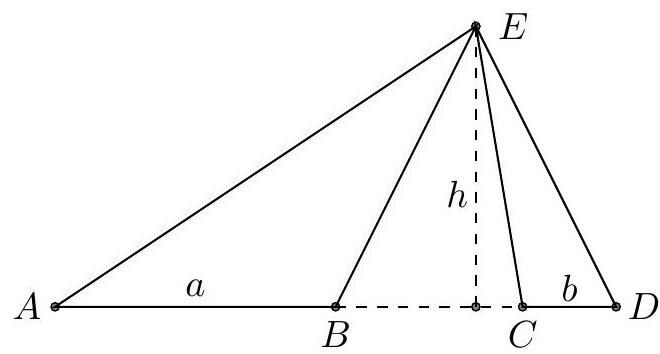
\includegraphics[max width=\textwidth, center]{2024_11_21_e9b4faa005d5be2cc318g-005}

Dowód: Dla dowodu spójrz na rysunek i zauważ przy tym, że

\[
P_{A B E}=\frac{1}{2} a h, P_{C D E}=\frac{1}{2} b h, \quad \text { stąd } \quad \frac{P_{A B E}}{P_{C D E}}=\frac{\frac{1}{2} a h}{\frac{1}{2} b h}=\frac{a}{b} .
\]

\section*{LEMAT 2}
Jeżeli trójkąty mają wspólną podstawę, a pozostałe wierzchołki leżą na prostej równoległej do tej podstawy, to trójkąty te mają równe pola.

\section*{Dowód:}
\begin{center}
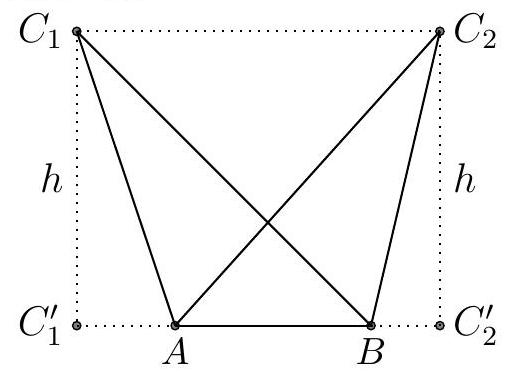
\includegraphics[max width=\textwidth]{2024_11_21_e9b4faa005d5be2cc318g-006(1)}
\end{center}

Rozpatrzmy trójkąty \(A B C_{1}\) i \(A B C_{2}\) o wspólnej podstawie \(A B\), przy czym \(\overline{C_{1} C_{2}} \| \overline{A B}\). Zauważmy, że wobec tego wysokości \(C_{1} C_{1}^{\prime}\) i \(C_{2} C_{2}^{\prime}\) opuszczone na prostą \(A B\) mają taką samą długość, którą oznaczmy \(h\), zaś długość podstawy \(A B\) oznaczmy \(a\). Wobec tego mamy \(P_{A B C_{1}}=\) \(\frac{1}{2} a h\), jak również \(P_{A B C_{2}}=\frac{1}{2} a h\).\\
Korzystając z powyższych dwóch lematów udowodnimy obecnie\\
TWIERDZENIE (Talesa) Jeżeli prosta równoległa do boku \(B C\) trójkąta \(A B C\) przecina boki \(A B\) i \(A C\) w punktach \(D\) i \(E\), to

\[
\mathrm{T}_{1}: \quad \frac{|A D|}{|D B|}=\frac{|A E|}{|E C|} \quad \mathrm{T}_{2}: \quad \frac{|A D|}{|A B|}=\frac{|D E|}{|B C|}
\]

Dowód: (tezy \(\mathrm{T}_{1}\) )\\
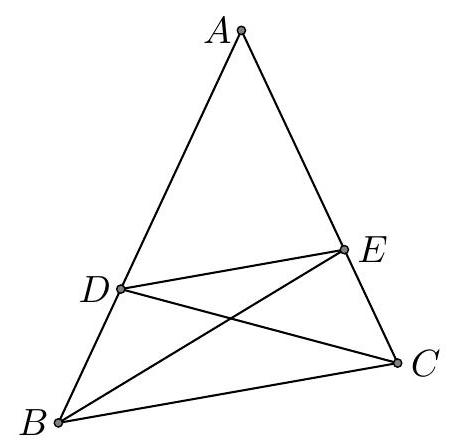
\includegraphics[max width=\textwidth, center]{2024_11_21_e9b4faa005d5be2cc318g-006}

Wobec tego mamy\\
\(\frac{|A D|}{|D B|}=\frac{P_{A D E}}{P_{D B E}}=\frac{P_{A D E}}{P_{E C D}}\).\\
Ostatnia równość wynika z lematu 2.\\
Zauważmy teraz, że trójkąty \(A E D\) i \(E C D\) mają podstawy leżące na jednej prostej i wspólny wierzchołek \(D\). Wobec tego mamy

\[
\frac{|A D|}{|D B|}=\frac{P_{A D E}}{P_{D B E}}=\frac{P_{A D E}}{P_{E C D}}=\frac{|A E|}{|E C|}
\]

przy czym ostatnia równość wynika z lematu 1. Z powyższego ciągu równości wynika, że

\[
\frac{|A D|}{|D B|}=\frac{|A E|}{|E C|}
\]

co jest końcem dowodu tezy \(T_{1}\).\\
Przed dowodem drugiej tezy, dla nabycia wprawy w pewnych przekształce-\\
niach, zróbmy ćwiczenie.

\begin{enumerate}
  \item W każdej z poniższych sytuacji ramiona kąta zostały przecięte dwiema lub trzema prostymi równoległymi. Wyznacz długości wskazanych odcinków.\\
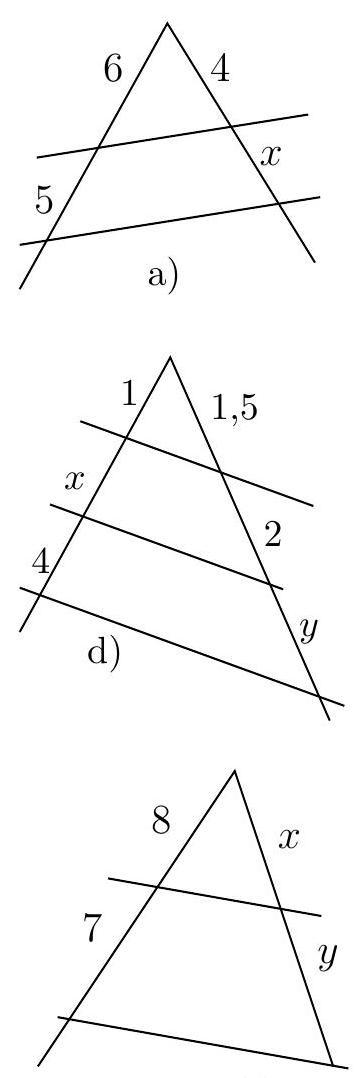
\includegraphics[max width=\textwidth, center]{2024_11_21_e9b4faa005d5be2cc318g-007}\\
g) \(x+y=30\)\\
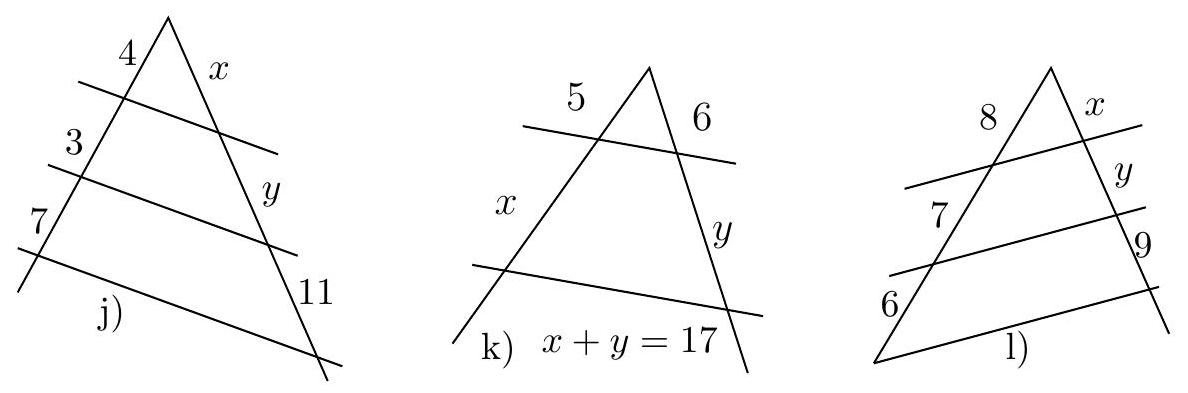
\includegraphics[max width=\textwidth, center]{2024_11_21_e9b4faa005d5be2cc318g-007(1)}
\end{enumerate}

Obecnie udowodnimy drugą tezę twierdzenia Talesa.\\
Dowód: (tezy T \(\mathrm{T}_{2}\) )\\
Mamy pokazać, że \(\quad \frac{|A D|}{|A B|}=\frac{|D E|}{|B C|}\).\\
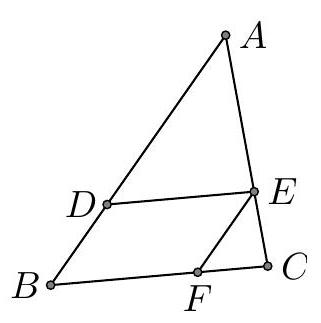
\includegraphics[max width=\textwidth, center]{2024_11_21_e9b4faa005d5be2cc318g-008(3)}

Na bokach trójkąta \(A B C\) obieramy punkty \(D, E, F\) tak, że\\
\(l_{D E} \| l_{B C}\), zaś \(l_{E F} \| l_{A B}\). Na mocy tezy \(\mathrm{T}_{1}\) mamy

\[
\frac{|C E|}{|E A|}=\frac{|C F|}{|F B|}, \text { bo } \overline{E F} \| \overline{A B}
\]

Dodając do obu stron powyższej równości liczbę 1 mamy

\[
\frac{|C E|}{|E A|}+1=\frac{|C F|}{|F B|}+1
\]

czyli

\[
\frac{|C E|+|E A|}{|E A|}=\frac{|C F|+|F B|}{|F B|}, \quad \text { czyli } \quad \frac{|C A|}{|E A|}=\frac{|C B|}{|F B|} .
\]

Ponieważ \(|B F|=|D E|\), bo \(B F E D\) jest równoległobokiem, więc \(\frac{|C A|}{|E A|}=\frac{|C B|}{|E D|}\), lub też biorąc odwrotności tych wyrażeń możemy zapisać \(\frac{|A E|}{|A C|}=\frac{|D E|}{|B C|}\), co kończy dowód tezy \(\mathrm{T}_{2}\).\\
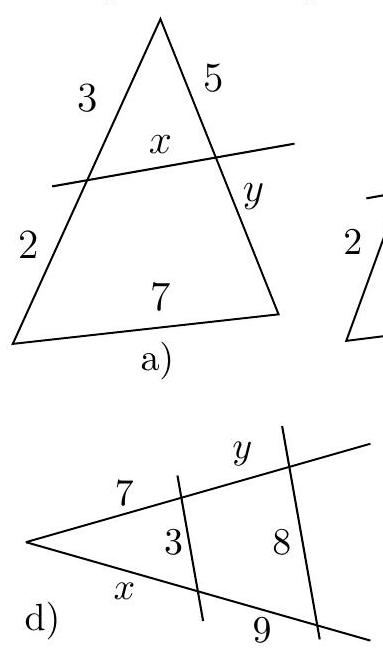
\includegraphics[max width=\textwidth, center]{2024_11_21_e9b4faa005d5be2cc318g-008}\\
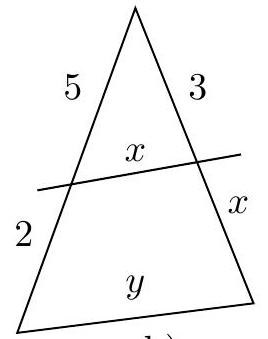
\includegraphics[max width=\textwidth, center]{2024_11_21_e9b4faa005d5be2cc318g-008(1)}\\
b)\\
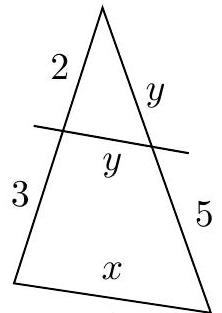
\includegraphics[max width=\textwidth, center]{2024_11_21_e9b4faa005d5be2cc318g-008(2)}\\
c)\\
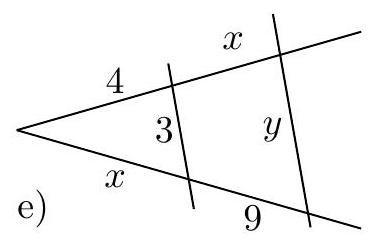
\includegraphics[max width=\textwidth, center]{2024_11_21_e9b4faa005d5be2cc318g-008(4)}\\
3. W trapezie \(A B C D\) o podstawach \(A B\) i \(C D\) mamy: \(|A B|=10,|C D|=5\), \(|A D|=4\). Przedłużenia ramion trapezu przecinają się w punkcie \(E\). Oblicz długość odcinka \(D E\).\\
4. W trójkącie \(A B C\) bok \(A B\) ma długość 6 . Na boku \(A C\) wybrano punkt \(M\) tak, że odcinek \(A M\) jest 3 razy dłuższy od odcinka \(M C\). Przez punkt \(M\) poprowadzono prostą równoległą do boku \(B C\), która przecięła bok \(A B\) w punkcie \(P\). Oblicz długości odcinków \(A P\) i \(P B\).\\
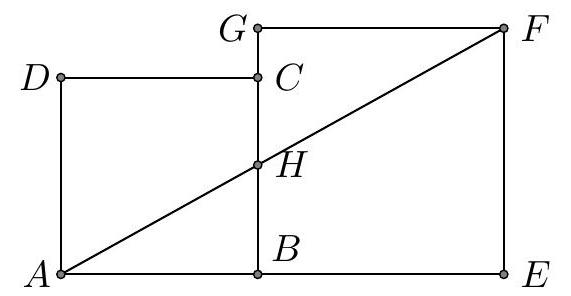
\includegraphics[max width=\textwidth, center]{2024_11_21_e9b4faa005d5be2cc318g-009(2)}\\
5. Na rysunku obok wierzchołek \(C\) kwadratu \(A B C D\), leży na boku \(B G\) kwadratu \(B E F G\). \(P_{A B C D}=49\), \(P_{B E F G}=64\). Oblicz \(P_{B E F H}\).\\
6. Na rysunku obok punkt \(D\) jest środkiem boku \(A B\), a odcinek \(D E\) jest równoległy do boku \(A C\). Oblicz obwody trójkątów \(A B C\) i \(D B E\).\\
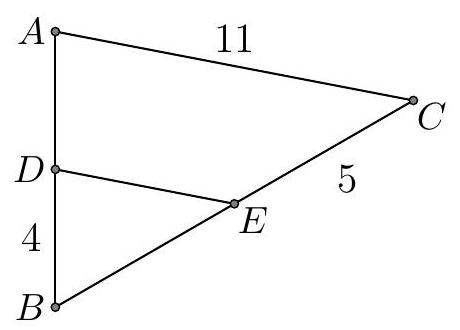
\includegraphics[max width=\textwidth, center]{2024_11_21_e9b4faa005d5be2cc318g-009}\\
7. W trójkącie \(A B C\) punkt \(D\) leży na boku \(B C\), punkt \(E\) leży na boku \(A C\), \(\overline{A B} \| \overline{E D},|C D|=|B D|=5,|A B|=12,|A E|=6\). Wyznacz obwód trójkąta \(C D E\).\\
8. W trójkącie \(A B C\) mamy: \(D \in \overline{A C}, E \in \overline{B C}, \overline{D E} \| \overline{A B},|D E|=5\), \(|A C|=9,|B E|=2 \cdot|C E|\). Wyznacz \(|A D|\) i \(|A B|\).\\
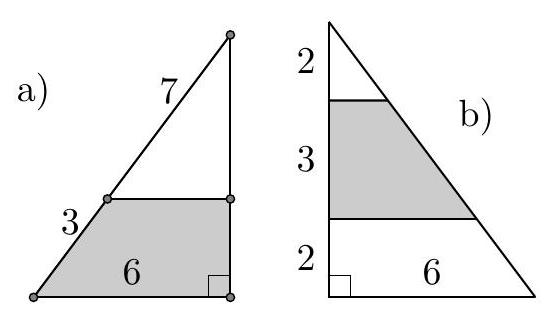
\includegraphics[max width=\textwidth, center]{2024_11_21_e9b4faa005d5be2cc318g-009(3)}\\
9. Oblicz pola zacieniowanych trapezów na rysunkach obok.\\
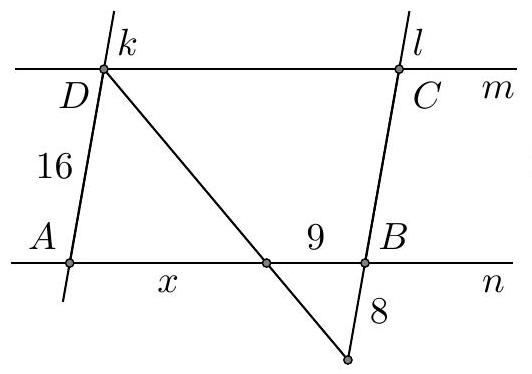
\includegraphics[max width=\textwidth, center]{2024_11_21_e9b4faa005d5be2cc318g-009(1)}\\
10. Na rysunku obok \(k \| l\) zaś \(m \| n\). Wyznacz \(x\).\\
11. W prostokącie \(A B C D\) na rysunku obok prosta \(E F\) jest równoległa do przekątnej \(A C\) i podzieliła bok \(A D\) na odcinki o podanych na rysunku długościach. Wyznacz pole prostokata \(A B C D\) oraz trapezu \(A C F E\).\\
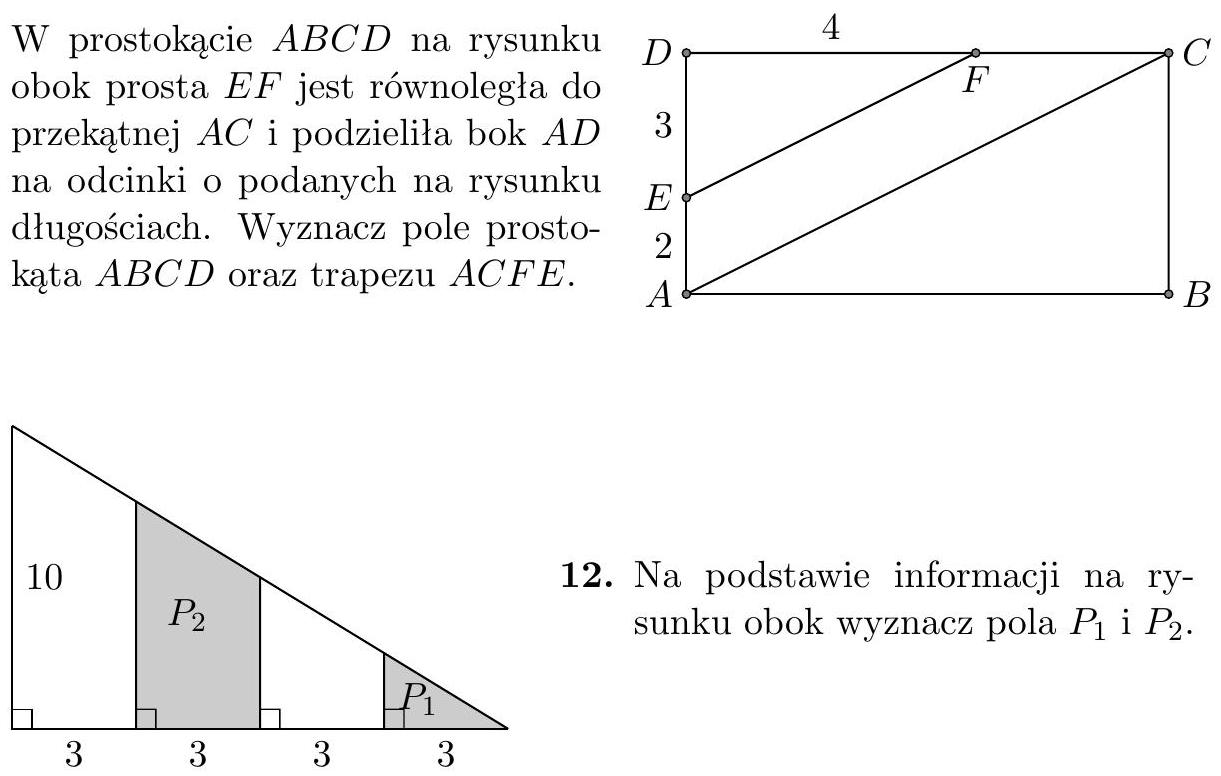
\includegraphics[max width=\textwidth, center]{2024_11_21_e9b4faa005d5be2cc318g-010(2)}\\
12. Na podstawie informacji na rysunku obok wyznacz pola \(P_{1}\) i \(P_{2}\).\\
13. W trójkącie \(A B C\) na rysunku obok kąt \(A C B\) jest prosty, zaś przeciwprostokątna ma długość 75 . Trójkąt ten został przecięty prostą \(E F\) równoległą do przeciwprostokątnej. Prosta ta podzieliła przyprostokątną \(A C\) na odcinki o podanych na rysunku długościach, odcinając od wyjściowego trójkąta trapez ABFE. Wyznacz:\\
a) długość wysokości trójkąta \(A B C\) opuszczonej na przeciwprostokątną,\\
b) długość krótszej podstawy trapezu,\\
c) pole trapezu,\\
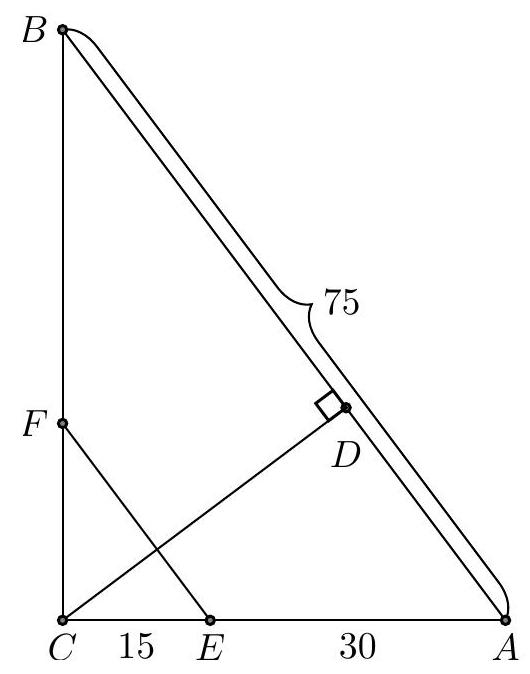
\includegraphics[max width=\textwidth, center]{2024_11_21_e9b4faa005d5be2cc318g-010(1)}\\
14. Odcinek \(D E\) na rysunku obok jest równoległy do przyprostokątnej \(A B\) trójkąta prostokątnego \(A B C\). Na podstawie podanych długości odcinków wyznacz \(E D, A B, P_{A B E D}\).\\
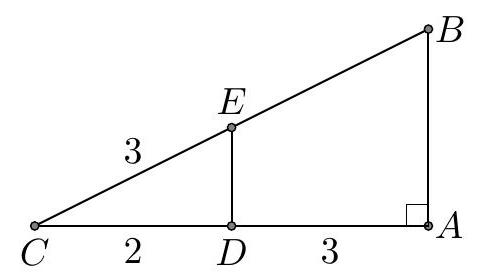
\includegraphics[max width=\textwidth, center]{2024_11_21_e9b4faa005d5be2cc318g-010}\\
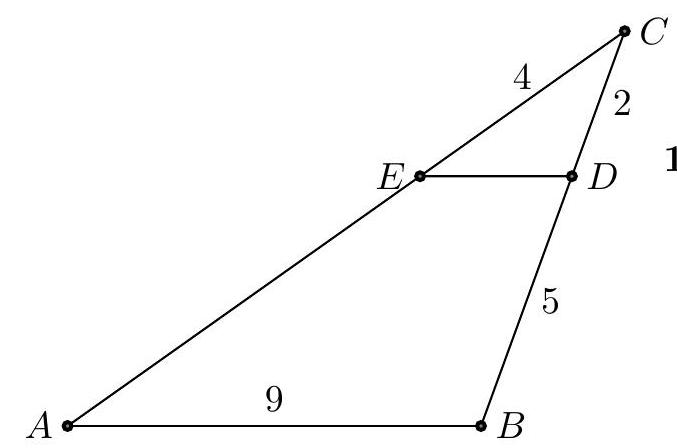
\includegraphics[max width=\textwidth, center]{2024_11_21_e9b4faa005d5be2cc318g-011}\\
15. Na rysunku obok \(\overline{D E} \| \overline{A B}\). Na podstawie podanych długości czterech odcinków wyznacz \(O b_{A B D E}\).\\
16. W trójkącie \(A B C\) na rysunku obok \(\overline{D E} \| \overline{A B},|C E|=|E B|=5\), \(|D E|=6,|D A|=7\). Wyznacz \(P_{A B E D}\).\\
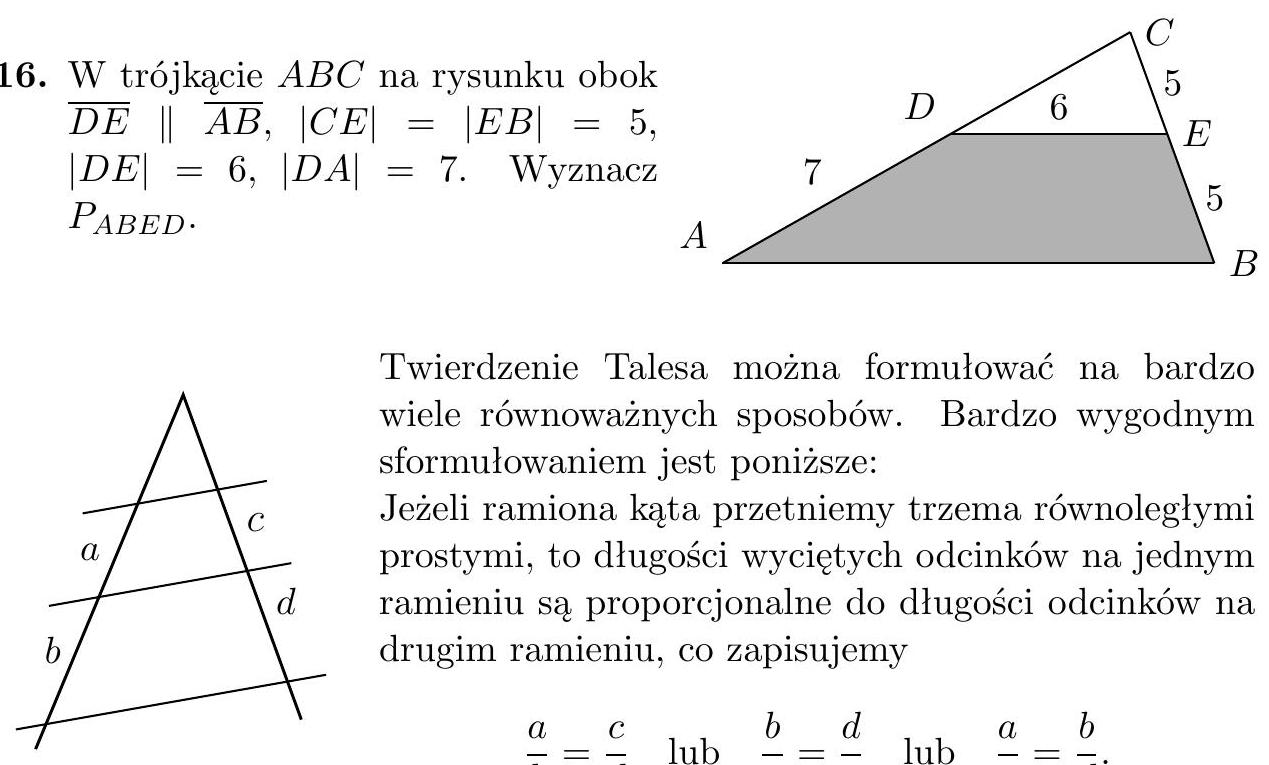
\includegraphics[max width=\textwidth, center]{2024_11_21_e9b4faa005d5be2cc318g-011(2)}

Twierdzenie Talesa można formułować na bardzo wiele równoważnych sposobów. Bardzo wygodnym sformułowaniem jest poniższe:\\
Jeżeli ramiona kąta przetniemy trzema równoległymi prostymi, to długości wyciętych odcinków na jednym ramieniu są proporcjonalne do długości odcinków na drugim ramieniu, co zapisujemy

\[
\frac{a}{b}=\frac{c}{d} \quad \text { lub } \quad \frac{b}{a}=\frac{d}{c} \quad \text { lub } \quad \frac{a}{c}=\frac{b}{d}
\]

\begin{enumerate}
  \setcounter{enumi}{16}
  \item Na obu rysunkach \(k\|l\| m\). Na podstawie podanych długości odcinków wyznacz \(x\).\\
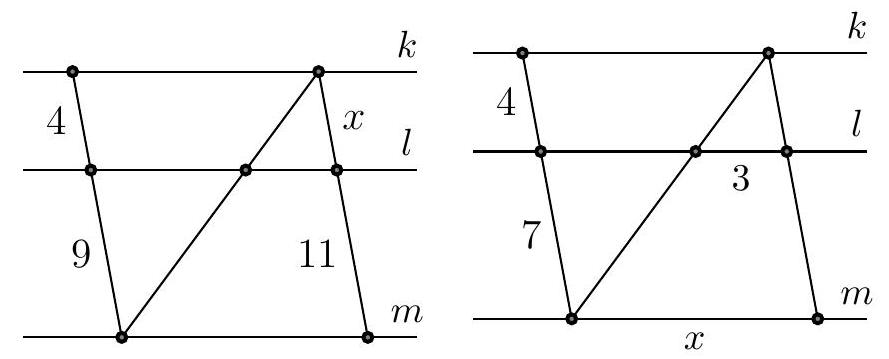
\includegraphics[max width=\textwidth, center]{2024_11_21_e9b4faa005d5be2cc318g-011(1)}
  \item Na poniższych dwóch rysunkach trójkąty \(A B C\) są prostokątne, zaś czworokąty \(C D E F\) są równoległobokami. Na podstawie podanych długości dwóch odcinków wyznacz \(P_{C D E F}\).\\
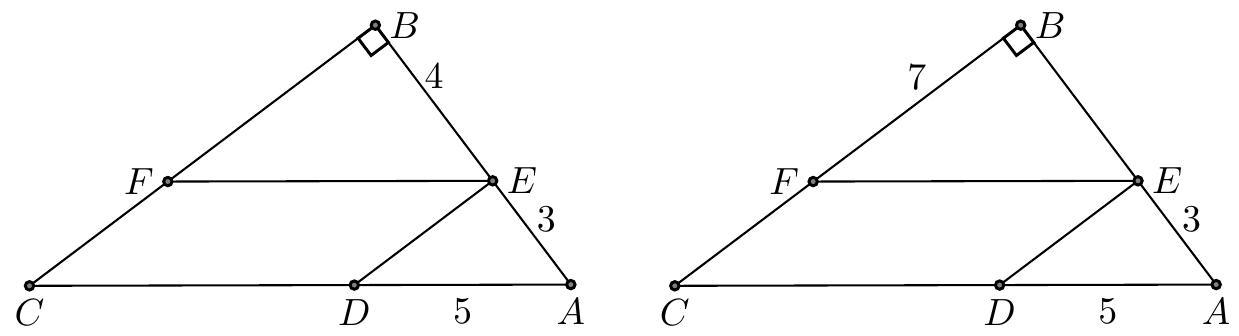
\includegraphics[max width=\textwidth, center]{2024_11_21_e9b4faa005d5be2cc318g-012(1)}
\end{enumerate}

Obecnie uzasadnimy, że prawdziwe jest również twierdzenie odwrotne do twierdzenia Talesa. A mianowicie

TWIERDZENIE Jeżeli w trójkącie \(A B C\) prosta \(k\) przecina boki \(A B\) i \(A C\) w punktach \(D\) i \(E\), a przy tym \(\frac{|A D|}{|D B|}=\frac{|A E|}{|E C|}\), to \(k \| l_{B C}\).\\
Dowód: (nie wprost) Przypuśćmy, że pomimo iż spełnione są założenia twierdzenia, to jednak \(l_{D E} \nVdash l_{B C}\). Wobec tego z aksjomatu 2, który mówi, że przez punkt nie leżący na danej prostej przechodzi tylko jedna prosta do niej równoległa, wynika że przez punkt \(D\) przechodzi jakaś inna prosta, która jest równoległa do \(l_{B C}\), i która przecina bok \(A C\) w jakimś punkcie. Oznaczmy sobie ten punkt \(E^{\prime}\). Wówczas na mocy tezy \(\mathrm{T}_{1}\)\\
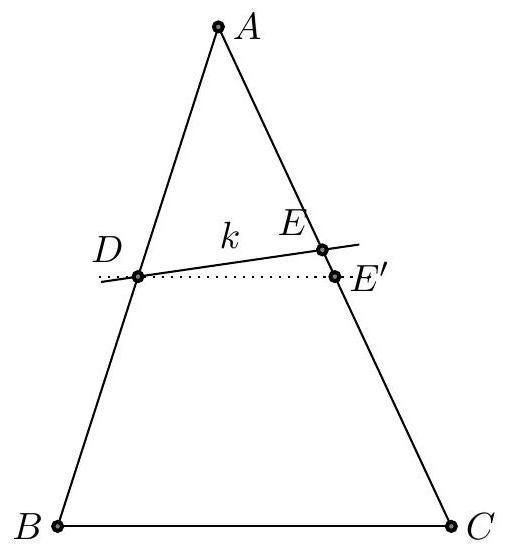
\includegraphics[max width=\textwidth, center]{2024_11_21_e9b4faa005d5be2cc318g-012}\\
twierdzenia Talesa mamy:

\[
\frac{|A D|}{|D B|}=\frac{\left|A E^{\prime}\right|}{\left|E^{\prime} C\right|}
\]

Z założenia naszego twierdzenia mamy \(\quad \frac{|A D|}{|D B|}=\frac{|A E|}{|E C|}\).\\
Z obu powyższych równości wynika, że \(\quad \frac{|A E|}{|E C|}=\frac{\left|A E^{\prime}\right|}{\left|E^{\prime} C\right|}\).\\
Ta ostatnia równość oznacza natomiast, że punkt \(E\) i punkt \(E^{\prime}\) to jest ten sam punkt czyli, że \(l_{D E}=l_{D E^{\prime}}\), czyli że jednak \(l_{D E} \| \overline{B C}\).\\
19. Punkty \(A, B, C, D\) i \(E\) są położone na dwóch półprostych tak jak na rysunku poniżej. Rozstrzygnij w każdym przypadku czy \(\overline{B E} \| \overline{C D}\), jeżeli długości odcinków są następujące\\
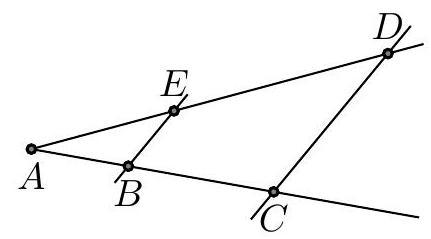
\includegraphics[max width=\textwidth, center]{2024_11_21_e9b4faa005d5be2cc318g-013(1)}\\
a) \(|A B|=2,|B C|=\frac{3}{2},|A E|=\frac{4}{3},|E D|=1\).\\
b) \(|A B|=2,|B C|=\frac{3}{2},|A E|=1,|E D|=\frac{4}{3}\).\\
c) \(|A C|=3,|A B|=2,|A D|=3 \sqrt{2}\), \(|A E|=2 \sqrt{2}\).\\
d) \(|A C|=2|A B|,|A D|=2|A E|\).\\
20. Zbadaj czy można rozstrzygnąć, a jeśli można\\
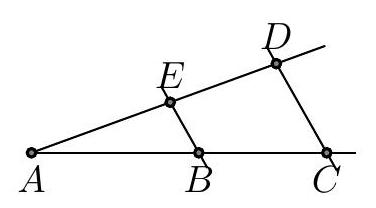
\includegraphics[max width=\textwidth, center]{2024_11_21_e9b4faa005d5be2cc318g-013}\\
to rozstrzygnij, czy \(\overline{E B} \| \overline{C D}\) gdy punkty \(A\), \(B, C, D\) i \(E\) są położone tak jak na rysunku obok i przy tym\\
a) \(|A B|=2,|A C|=5,|E B|=3,|D C|=\frac{15}{2}\).\\
b) \(|A E|=1,|E D|=6,|E B|=3,|D C|=9\)\\
21. W trójkącie \(A B C\) na boku \(A C\) obrano punkt \(D\), a na boku \(B C\) punkt \(E\) tak, że \(\frac{|C D|}{|A D|}=\frac{|C E|}{|E B|}=\frac{2}{5},|D E|=78\). Wyznacz \(|A B|\).\\
22. W trójkącie \(A B C D \in \overline{A C}, E \in \overline{B C},|A C|=3|C D|,|B E|=2|C E|\), \(|A B|=16\). Wyznacz \(|D E|\).

Z twierdzenia odwrotnego do twierdzenia Talesa wynika poniższe twierdzenie o odcinku łączącym środki boków trójkąta.\\
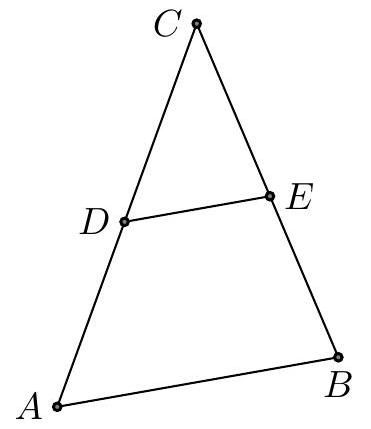
\includegraphics[max width=\textwidth, center]{2024_11_21_e9b4faa005d5be2cc318g-013(2)}

TWIERDZENIE Odcinek łączący środki dwóch boków trójkąta jest równoległy do trzeciego boku, a jego długość równa jest połowie długości trzeciego boku.\\
Dowód: Ponieważ \(D\) jest środkiem odcinka \(C A\), zaś \(E\) środkiem odcinka \(C B\), wobec tego

\[
1=\frac{|C D|}{|D A|}=\frac{|C E|}{|E B|}
\]

więc na mocy twierdzenia odwrotnego do twierdzenia Talesa \(\overline{D E} \| \overline{A B}\). Z drugiej tezy twierdzenia Talesa mamy \(\frac{|D C|}{|A C|}=\frac{|D E|}{|A B|}\), a ponieważ \(|A D|=|D C|\) czyli \(\frac{|D C|}{|A C|}=\frac{1}{2}\), więc \(\frac{|D E|}{|A B|}=\frac{1}{2}\) czyli \(|D E|=\frac{1}{2}|A B|\).\\
23. Obwód trójkąta wynosi 12 cm . Środki boków trójkąta połączono odcinkami tworząc trójkąt. Wyznacz obwód otrzymanego trójkąta.\\
24. W trójkącie o bokach długości \(a, b, c\) łączymy środki kolejnych boków uzyskując trójkąt. Oblicz obwód uzyskanego trójkąta.\\
25. Długości przyprostokątnych trójkąta prostokątnego równe są \(a\) i \(b\). Odcinek łączący ich środki dzieli ten trójkąt na czworokąt i trójkąt prostokątny.\\
a) Uzasadnij, że czworokąt ten jest trapezem.\\
b) Wyznacz pole tego czworokąta (spróbuj w pamięci).\\
c) Wyznacz wysokość wyjściowego trójkąta opuszczoną na przeciwprostokątną.\\
d) Wyznacz długość krótszej podstawy trapezu.\\
e) Wyznacz wysokość uzyskanego trapezu licząc tylko odpowiednie pola.\\
26. W trójkącie równobocznym o boku długości a połączono środki dwóch boków odcinkiem. Oblicz obwód powstałego czworokąta.\\
27. W trójkącie o podstawie \(a\) i wysokości \(h\) opuszczonej na tę podstawę prowadzimy prostą równoległą do tej podstawy i przechodzącą przez środki ramion tego trójkąta. Wyznacz pole uzyskanego trapezu. Oblicz jakim procentem wyjściowego trójkąta jest pole uzyskanego trapezu.\\
28. Uzasadnij, że odcinki łączące środki kolejnych boków czworokąta tworzą równoległobok. wsk. Co trzeba dorysować, aby to uzasadnić?\\
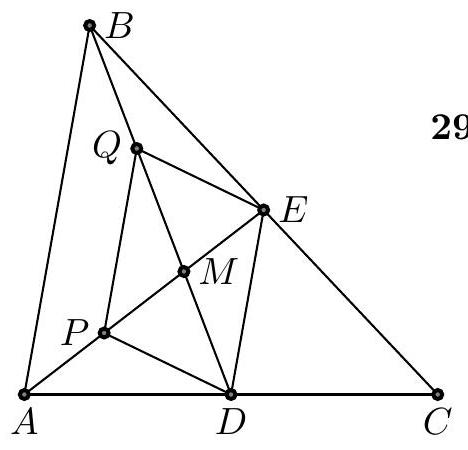
\includegraphics[max width=\textwidth, center]{2024_11_21_e9b4faa005d5be2cc318g-014}\\
29. W trójkącie \(A B C\) na rysunku obok poprowadzono środkowe \(A E\) i \(B D\), które przecinają się w punkcie \(M\). W trójkącie \(A M B\) punkty \(P\) i \(Q\) są środkami boków. Pokaż, że czworokąt \(D E Q P\) jest równoległobokiem.\\
30. Dany jest prostokąt o bokach długości \(a\) i \(b\). Łączymy kolejno środki boków tego prostokąta.\\
a) Uzasadnij, że uzyskany tym sposobem czworokąt jest rombem\\
b) Wyznacz pole powierzchni tego rombu (w pamięci)\\
c) Wyznacz wysokość tego rombu\\
31. W czworokącie łączymy środki jego boków uzyskując w ten sposób czworokąt będący równoległobokiem. Oblicz jakim procentem wyjściowego czworokąta jest pole uzyskanego równoległoboku.\\
32. W trapezie prostokątnym dłuższa podstawa ma długość \(a\), krótsza ma długość \(b\). Ramię o długości \(d\) jest prostopadłe do obu podstaw. Łączymy kolejno środki boków tego trapezu.\\
a) Uzasadnij, że uzyskany czworokąt jest równoległobokiem.\\
b) Wyznacz długości boków tego równoległoboku.\\
c) Wyznacz obie wysokości równoległoboku oraz pole powierzchni.\\
33. W czworokącie \(A B C D\) punkty \(E, F, G\) i \(H\) są kolejno środkami boków \(A B, B C, C D\) i \(D A\). Przekątna \(A C\) wyjściowego czworokąta ma długość \(d\) i podzieliła równoległobok \(E F G H\) na dwa równoległoboki. Wysokość trójkąta \(A C D\) opuszczona na podstawę \(A C\) ma długość \(h\).\\
a) Oblicz pole trójkąta \(D H G\).\\
b) Oblicz pole tego równoległoboku, który leży w trójkącie \(A C D\).

34* Dany jest trójkąt ostrokątny \(A B C\) o podstawie \(A B\) i wierzchołku \(C\). Prowadzimy dwusieczne kątów zewnętrznych \(\Varangle A\) i \(\Varangle B\). Rzutujemy prostopadle punkt \(C\) na każdą z tych dwusiecznych. Oznaczmy punkty rzutowania przez \(P\) i \(Q\). Pokaż, że \(|P Q|=\frac{1}{2}(|A B|+|B C|+|C A|)\). wsk. zrób staranny rysunnek

TWIERDZENIE Odcinek łączący środki ramion trapezu jest równoległy do obu podstaw, a jego długość jest równa połowie sumy długości podstaw.

\section*{Dowód.}
Wpierw zauważmy, że\\
\(\overline{A B} \| \overline{C D}\) - jako podstawy trapezu, \(\Varangle C F D=\Varangle B F G-\) kąty wierzchołkowe, \(\Varangle D C F=\Varangle G B F-\) kąty naprzemianległe, \(|C F|=|F B|-\) z założenia.\\
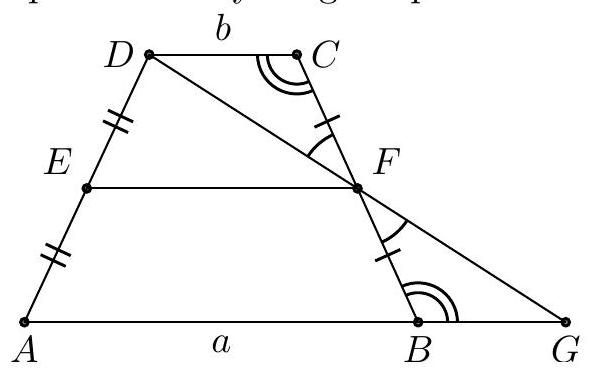
\includegraphics[max width=\textwidth, center]{2024_11_21_e9b4faa005d5be2cc318g-015}

Wobec tego na mocy KBK przystawania trójkątów \(\triangle D C F \equiv \triangle G B F\). Z tego wynika, że

\[
|C D|=|B G|(\text { czyli }|B G|=b) \text { oraz }|D F|=|F G|
\]

jako długości odpowiadających sobie boków w trójkątach przystających.\\
Czyli \(|A G|=a+b\). Wobec tego odcinek \(E F\) łączy środki boków trójkąta \(A G D\), więc jest on równoległy do boku \(A G\) a jego długość równa jest połowie długości boku \(A G\) czyli \(\frac{1}{2}(a+b)\).\\
35. Odcinek łączący środki ramion trapezu ma długość 7 cm , a jedna z jego podstaw dłuższa jest od drugiej o 4 cm . Wyznacz długości podstaw.\\
36. Stosunek długości podstaw w trapezie równy jest \(2: 3\), a odcinek łączący środki ramion trapezu ma długość 5m. Wyznacz długość podstaw tego trapezu.

TWIERDZENIE Jeżeli prosta przechodzi przez środek jednego ramienia trapezu i jest równoległa do podstaw trapezu, to przechodzi ona również przez środek drugiego ramienia trapezu.\\
37. Udowodnij powyższe twierdzenie.\\
38. Punkty \(A, B, C\) leżą na jednaj prostej, w tej właśnie kolejności. Trójkąty \(A B D\) i \(B C E\) są równoboczne, przy czym punkty \(D\) i \(E\) leżą po jednej stronie prostej \(A B\). Niech \(F\) będzie środkiem odcinka \(A B, G\) - środkiem odcinka \(B C\), zaś \(H\) - środkiem odcinka \(D E\). Uzasadnij, że trójkąt \(F G H\) jest równoboczny.\\
39. Podstawy trapezu mają długości równe \(a\) i \(b\), przy czym \(a>b\). Wyznacz długość odcinka jaki przekątne tego trapezu wycinają na prostej łączącej środki ramion tego trapezu.\\
40. Wysokość poprowadzona z wierzchołka kąta rozwartego w trapezie równoramiennym dzieli jego podstawę na odcinki o długościach \(a\) i \(b, a>b\). Wyznacz długość odcinka łączącego środki ramion tego trapezu.\\
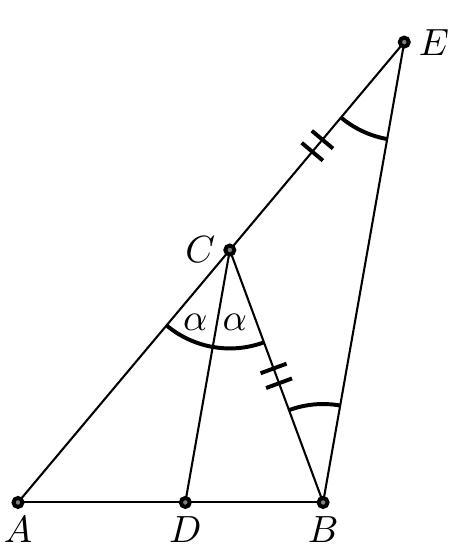
\includegraphics[max width=\textwidth, center]{2024_11_21_e9b4faa005d5be2cc318g-016}

TWIERDZENIE Jeżeli \(A B C\) jest dowolnym trójkątem, wówczas dwusieczna kąta np. \(\Varangle C\) dzieli przeciwległy bok \(A B\) na dwa odcinki o długościach proporcjonalnych do długości boków \(A C\) i \(B C\), to znaczy \(\frac{|A C|}{|C B|}=\frac{|A D|}{|B D|}\) czyli \(\frac{|A C|}{|A D|}=\frac{|C B|}{|B D|}\).\\
Dowód:\\
Niech \(C D\) będzie dwusieczną kąta przy wierzchołku \(C\). Poprowadźmy prostą \(A C\), zaś przez punkt \(B\) poprowadźmy prostą równoległą do dwusiecznej \(C D\). Niech prosta ta przecina prostą \(A C\) w punkcie \(E\).

Wówczas kąty \(\Varangle A C D\) i \(\Varangle C E B\) są kątami odpowiadającymi, a kąty \(\Varangle D C B\) i \(\Varangle C B E\) kątami naprzemianległymi. Ponieważ \(\Varangle A C D=\Varangle D C B\), bo \(C D\) jest dwusieczną, więc w trójkącie \(B C E\) kąty \(\Varangle C B E\) i \(\Varangle C E B\) są równe, czyli jest to trójkąt równoramienny, w którym \(|C B|=|C E|\). Mamy więc następującą sytuację: w trójkącie \(A B E\) zachodzi \(\overline{C D} \| \overline{E B}\), więc na mocy twierdzenia Talesa \(\frac{|A C|}{|C E|}=\frac{|A D|}{|D B|}\), a ponieważ \(|C E|=|C B|\) więc \(\frac{|A C|}{|C B|}=\frac{|A D|}{|D B|}\) czyli \(\frac{|A C|}{|A D|}=\frac{|C B|}{|D B|}\).

Ma miejsce również twierdzenie odwrotne:

TWIERDZENIE Niech \(A B C\) będzie dowolnym trójkątem. Z wierzchołka \(C\) prowadzimy prostą, która dzieli przeciwległy bok \(A B\) w punkcie \(D\) na dwa odcinki o długościach proporcjonalnych do długości boków \(A C\) i \(B C\) \(\operatorname{tzn}\), że \(\frac{|C A|}{|C B|}=\frac{|A D|}{|B D|}\). Wówczas ta prosta jest dwusieczną kąta \(C\).\\
UWAGA Dwusieczna kąta jest to półprosta wychodząca z wierzchołka kąta. Często w zadaniach o trójkącie używamy słowa dwusieczna rozumiejąc przez to odcinek zawarty w dwusiecznej kąta ograniczony wierzchołkiem kąta i punktem przecięcia dwusiecznej z przeciwległym bokiem.\\
41. W trójkącie \(A B C\) dane są: \(|A B|=5,|B C|=8, \Varangle A B C=120^{\circ}\). Korzystając z twierdzenia o dwusiecznej wyznacz długość dwusiecznej kąta \(A B C\).\\
42. Uzasadnij, że jeżeli w trójkącie \(A B C\) środkowa \(B D\) jest dwusieczną, to on jest równoramienny. wsk. skorzystaj z twierdzenia o dwusiecznej.\\
43. Wyznacz długość \(d\) dwusiecznej kąta prostego w trójkącie o przyprostokątnych długości \(a\) i \(b\). wsk. skorzystaj z dowodu twierdzenia o dwusiecznej.\\
44. W równoległoboku \(A B C D\) punkt \(A_{1}\) jest środkiem boku \(A B\), a \(C_{1}\) środkiem boku \(C D\). Udowodnij, że odcinki \(A_{1} C\) i \(A C_{1}\) przecinając przekątną \(B D\) dzielą ją na trzy odcinki równej długości.

45* Pokaż, że punkt przecięcia przekątnych w trapezie dzieli każdą z nich na odcinki, których długości są proporcjonalne do długości odpowiednich podstaw.

46* Wierzchołki \(A\) i \(D\) dwóch trójkątów o wspólnej podstawie \(B C\) leżą po tej samej stronie podstawy. Z dowolnego punktu podstawy wykreślono\\
jedną prostą równoległą do \(A B\), która przecina \(A C\) w punkcie \(F\), oraz (z tego samego punktu) drugą prostą równoległą do \(B D\), która przecina \(D C\) w punkcie \(G\). Pokaż, że \(\overline{F G} \| \overline{A D}\).\\
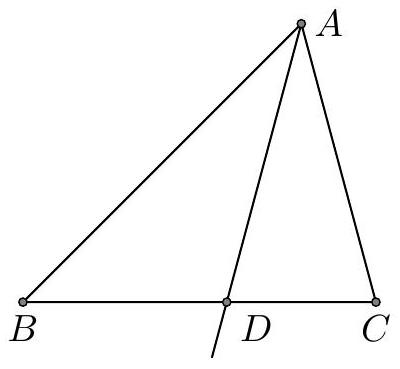
\includegraphics[max width=\textwidth, center]{2024_11_21_e9b4faa005d5be2cc318g-018(1)}\\
47. W trójkącie \(A B C\), na rysunku obok, poprowadzono dwusieczną \(A D \rightarrow\). Niech \(A B=c\), \(B C=a, A C=b\). Wyznacz długości odcinków \(A D\) i \(D B\) w zależności od \(a, b, c\).\\
48. W trójkącie równoramiennym o podstawie długości \(a\), zaś ramionach długości \(b\) prowadzimy dwusieczną kąta przy podstawie. Przecina ona jedno z ramion trójkąta. Wyznacz długości odcinków na jakie dwusieczna podzieliła to ramię.\\
49. W trójkącie równoramiennym ramiona mają długość \(a\), zaś podstawa ma długość \(b\). Dwusieczne kątów (wewnętrznych) przy podstawie przecinają ramiona trójkąta w punktach \(A\) i \(B\). Wyznacz długość odcinka \(A B\).\\
50. W trójkącie ostrokątnym \(A B C\) wysokość \(C D\) podzieliła podstawę \(A B\) na odcinki o długościach: \(|A D|=3,|D B|=5\). Bok \(B C\) ma długość 7. Symetralna podstawy \(A B\) przecina bok \(B C\) w punkcie \(F\). Wyznacz \(C F, C D\) oraz \(P_{A C F}\).\\
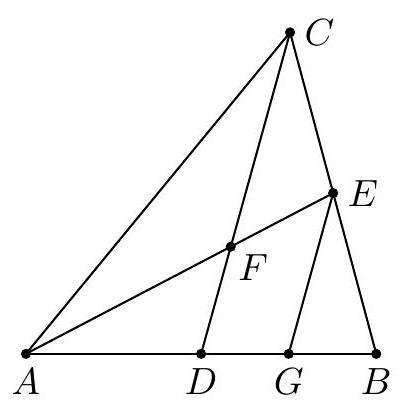
\includegraphics[max width=\textwidth, center]{2024_11_21_e9b4faa005d5be2cc318g-018}

TWIERDZENIE Punkt w którym przecinają się dwie środkowe w trójkącie dzieli każdą z nich w stosunku 2:1 (począwszy od wierzchołka). Wszystkie trzy środkowe w trójkącie przecinają się w jednym punkcie.

\section*{Dowód:}
Niech \(C D\) i \(A E\) będą środkowymi przecinającymi się w punkcie \(F\). Przez punkt \(E\) poprowadźmy odcinek \(E G\) równoległy do \(F D\).\\
Wpierw rozważmy trójkąt \(D B C\), w którym po pierwsze \(|B E|=|C E|\), bo \(E\) jest środkiem odcinka \(B C\), a po drugie \(\overline{G E} \| \overline{C D}\), bo tak wybraliśmy sobie punkt \(G\). Wobec tego na mocy twierdzenia Talesa mamy \(1=\frac{|B E|}{|C E|}=\frac{|B G|}{|G D|}\). Z tego wynika, że punkt \(G\) jest środkiem odcinka \(D B\). Ponieważ \(D\) jest środkiem odcinka \(A B\), więc wobec tego \(|A D|=2|D G|\).\\
Rozważmy teraz trójkąt \(A G E\), w którym \(\overline{D F} \| \overline{G E}\), wobec tego na mocy\\
twierdzenia Talesa mamy

\[
\frac{|A F|}{|F E|}=\frac{|A D|}{|D G|}=\frac{2|D G|}{|D G|}=\frac{2}{1}
\]

Pokazaliśmy zatem, że punkt \(F\), w którym przecinają się środkowe \(A E\) i \(C D\) dzieli środkową \(A E\) w stosunku 2: 1. W podobny sposób, czyli prowadząc przez punkt \(D\) równoległą do środkowej \(A E\) możemy uzasadnić, że punkt \(F\) dzieli środkową \(C D\) w stosunku 2:1. Ponieważ tylko jeden punkt \(F\) może podzielić środkową \(C D\) tak, że \(\frac{|C F|}{|F D|}=\frac{2}{1}\), więc z tego wynika, że trzecia środkowa trójkąta \(A B C\) wychodząca z wierzchołka \(B\), również przechodzi przez punkt \(F\).

\section*{DEFINICJA}
Punkt, w którym przecinają się środkowe trójkąta nazywamy środkiem ciężkości trójkąta i oznaczamy go zazwyczaj literą \(G\) (skrót od grawitacja).\\
Fizycznie oznacza to, że gdybyśmy trójkąt wykonali z jednorodnej płyty i podparli ten trójkąt - umieszczony poziomo - w punkcie \(G\), to pozostałby on w stanie równowagi. Podobnie środek odcinka jest jego środkiem ciężkości, co oznacza, że gdybyśmy wzięli jednorodny pręt i w pozycji poziomej podparli go w środku, to pozostałby on w stanie równowagi.\\
51. Na boku \(B C\) trójkąta \(A B C\) obrano punkt \(K\) tak, że \(B K: K C=2: 1\). W jakim stosunku środkowa \(C C_{1}\) dzieli odcinek \(A K\) ?\\
52. W trójkącie \(A B C\) kąt \(C\) jest prosty, \(|A C|=12,|B C|=16\). Niech \(D\) będzie środkiem boku \(A B\), zaś \(G\) środkiem ciężkości trójkąta \(A B C\). Wyznacz \(P_{A D G}\) oraz odległość punktu \(G\) od każdego z boków trójkąta.\\
53. W trójkącie ostrokątnym \(A B C\) długości boków są następujące: \(|A B|=16,|B C|=20,|C A|=24\). Wyznacz wysokość \(h_{c}\) wychodzącą z wierzchołka \(C\) oraz \(P_{A B C}\). Wyznacz odległość środka ciężkości \(G\) trójkąta \(A B C\) od boków trójkąta.

\section*{Wskazówki i odpowiedzi.}
\begin{enumerate}
  \item a) \(3 \frac{1}{3}\), b) \(x=2 \frac{1}{7}, y=5 \frac{3}{5}\), \(y=9 \frac{3}{11}\), l) \(x=12, y=10 \frac{1}{2}\)\\
c) \(\left.x=12 \frac{1}{4}, y=26 \frac{2}{7} \mathrm{~d}\right) x=\frac{4}{3}\),
  \item a) \(x=4 \frac{1}{5}, y=3 \frac{1}{3}\), b) \(x=1 \frac{1}{5}\),\\
\(y=6\), e) \(x=7 \frac{1}{2}, y=3 \frac{3}{4}\),\\
\(y=1 \frac{17}{25}\) c) \(x=8 \frac{1}{3}, y=3 \frac{1}{3}\),\\
f) \(x=6\), g) \(x=16, y=14\),\\
d) \(x=5 \frac{2}{5}, y=11 \frac{2}{3}\), e) \(x=6\),\\
h) \(x=4, y=4 \frac{1}{2}\), i) \(x=6, y=18, \quad y=7 \frac{1}{2}\)\\
j) \(\left.x=6 \frac{2}{7}, y=4 \frac{5}{7}, \mathrm{k}\right) x=7 \frac{8}{11}\),
  \item \(|D E|=4\)
  \item \(|A P|=4 \frac{1}{2},|P B|=1 \frac{1}{2}\)\\
d) \(p=\frac{1}{2} \sqrt{a^{2}+b^{2}}\), e) \(h=\frac{a b}{2 \sqrt{a^{2}+b^{2}}}\)
  \item \(|B H|=\frac{56}{15}, P_{B E F H}=46 \frac{14}{15}\)
  \item \(O b_{A B C}=29, O b_{D B E}=14 \frac{1}{2}\)
  \item \(O b_{C D E}=17\)
  \item \(|A D|=6,|A B|=15\)
  \item a) \(P=12 \frac{6}{25}\), b) \(P=9\)
  \item \(x=18\)
  \item \(P_{A B C D}=33 \frac{1}{3}, P_{A C F E}=10 \frac{2}{3}\)
  \item \(P_{1}=3 \frac{3}{4}, P_{2}=18 \frac{3}{4}\)
  \item a) \(|C D|=36\), b) \(|E F|=25\),\\
c) \(P_{A B F E}=1200\)
  \item \(|E D|=\sqrt{5},|A B|=\frac{5}{2} \sqrt{5}\),\\
\(P_{A B E D}=\frac{21}{4} \sqrt{5}\)
  \item \(A E=10, E D=\frac{18}{7}\),\\
\(O b_{A B D E}=26 \frac{4}{7}\)
  \item \(P_{A B E D}=18 \sqrt{6}\)
  \item a) \(4 \frac{8}{9}\), b) \(8 \frac{1}{4}\)
  \item a) \(P_{C D E F}=16\), b) \(P_{C D E F}=21\)
  \item a) są, b) nie są, c) są, d) są
  \item a) można - są równoległe,\\
b) można - nie są równoległe
  \item \(|A B|=273\)
  \item \(|D E|=5 \frac{1}{3}\)
  \item \(O b=6\)
  \item \(O b=\frac{1}{2}(a+b+c)\)
  \item b) \(P=\frac{3}{8} a b\), c) \(h=\frac{a b}{\sqrt{a^{2}+b^{2}}}\),
  \item \(2 \frac{1}{2} a\)
  \item \(P=\frac{3}{8} a h, 75 \%\)
  \item b) \(P=\frac{1}{2} a b\), c) \(h=\frac{a b}{\sqrt{a^{2}+b^{2}}}\)\\
31.50\%
  \item b) \(\frac{1}{2} \sqrt{d^{2}+b^{2}}, \frac{1}{2} \sqrt{a^{2}+d^{2}}\),\\
c) \(h_{1}=\frac{a b+b d}{\sqrt{d^{2}+b^{2}}}, h_{2}=\frac{a d+b d}{\sqrt{d^{2}+a^{2}}}\)
  \item a) \(P_{D H G}=\frac{1}{8} d h\), b) \(\frac{1}{4} d h\)\\
35.5 i 9
  \item 4 i 6
  \item \(\frac{1}{2}(a-b)\)
  \item \(a\)
  \item \(d=\frac{40}{13}\)
  \item \(d=\frac{a b \sqrt{2}}{a+b}\)
  \item wsk. co trzeba dorysować?
  \item \(A D=\frac{b c}{a+b}, D B=\frac{a c}{a+b}\)
  \item \(\frac{a b}{a+b}, \frac{b^{2}}{a+b}\)
  \item \(|A B|=\frac{a b}{a+b}\)
  \item \(|C F|=\frac{7}{5},|C D|=2 \sqrt{6}\),\\
\(P_{A C F}=\frac{8}{5} \sqrt{6}\)\\
51.3:1
  \item \(P_{A D G}=16, d(G, A B)=\frac{16}{5}\),\\
\(d(G, A C)=\frac{16}{3}, d(G, B C)=4\),
  \item \(h_{c}=\frac{15}{2} \sqrt{7}, \quad P_{A B C}=60 \sqrt{7}\),\\
\(d(G, A B)=\frac{5}{2} \sqrt{7}, d(G, A C)=\frac{5}{3} \sqrt{7}\),\\
\(d(G, B C)=\frac{1}{2} \sqrt{7}\).
\end{enumerate}

\section*{Rozdział 2}
\section*{TRÓJKĄTY PODOBNE}
\section*{DEFINICJA}
Dwa trójkąty nazywamy podobnymi jeżeli mają takie same kąty.\\
Fakt, że trójkąt \(A B C\) jest podobny do trójkąta \(P Q R\) będziemy zapisywać \(\triangle A B C \sim \triangle P Q R\). Zapis ten oznacza równość odpowiednich kątów, a mianowicie\\
\(\Varangle A=\Varangle P, \Varangle B=\Varangle Q, \Varangle C=\Varangle R\).\\
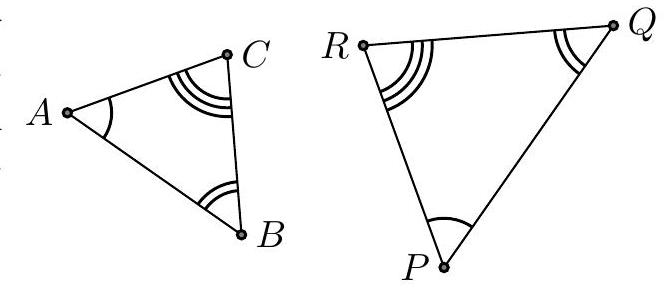
\includegraphics[max width=\textwidth, center]{2024_11_21_e9b4faa005d5be2cc318g-021}

\begin{enumerate}
  \item Uzasadnij, że wysokość opuszczona na przeciwprostokątną trójkąta prostokątnego dzieli ten trójkąt na trójkąty podobne, przy czym oba z nich są podobne do wyjściowego trójkąta. Zapisz zgodnie z konwencją podaną w definicji podobieństwa trójkątów odpowiednie związki.\\
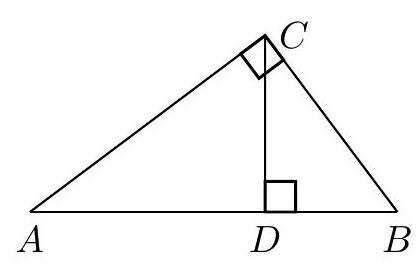
\includegraphics[max width=\textwidth, center]{2024_11_21_e9b4faa005d5be2cc318g-021(1)}
  \item Uzasadnij, że zacieniowany trójkąt na rysunku poniżej jest podobny do trójkąta \(A B C\).\\
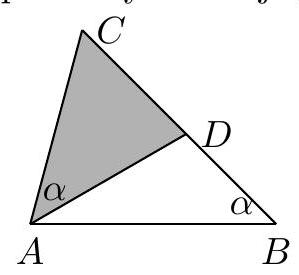
\includegraphics[max width=\textwidth, center]{2024_11_21_e9b4faa005d5be2cc318g-021(2)}
  \item Narysuj dowolny prostokąt. Poprowadź linie wzdłuż których należy go rozciąć aby otrzymać\\
a) 2 trójkąty podobne\\
b) 3 trójkąty podobne\\
c) 4 trójkąty podobne\\
d) 5 trójkątów podobnych\\
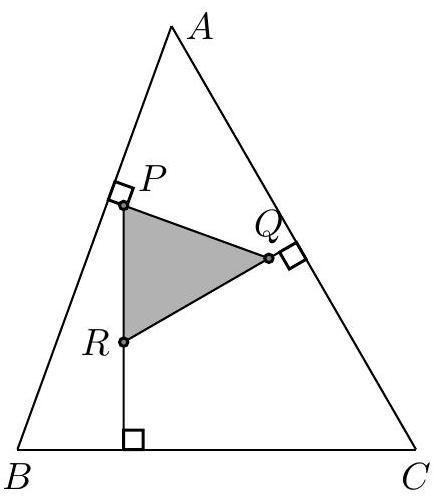
\includegraphics[max width=\textwidth, center]{2024_11_21_e9b4faa005d5be2cc318g-022}
  \item Boki trójkąta \(A B C\) na rysunku obok zostały przecięte prostymi prostopadłymi do jego boków, tworząc trójkąt \(P Q R\). Uzasadnij, że trójkąt \(P Q R\), jest podobny do trójkąta \(A B C\) i zapisz odpowiedni związek.
  \item W trapezie \(A B C D\) o podstawach \(A B\) i \(C D\) przekątne \(A C\) i \(B D\) przecinają się w punkcie \(O\). Uzasadnij, że \(\triangle A B O \sim \triangle C D O\).
  \item Wyznacz miary kątów trójkąta równoramiennego, jeżeli dwusieczna kąta przy podstawie odcina trójkąt podobny do wyjściowego trójkąta.
  \item W trójkącie \(A B C\) na rysunku obok poprowadzono dwie wysokości. Które z trójkątów są podobne do trójkąta \(A D C\) ? Zapisz odpowiednie związki.\\
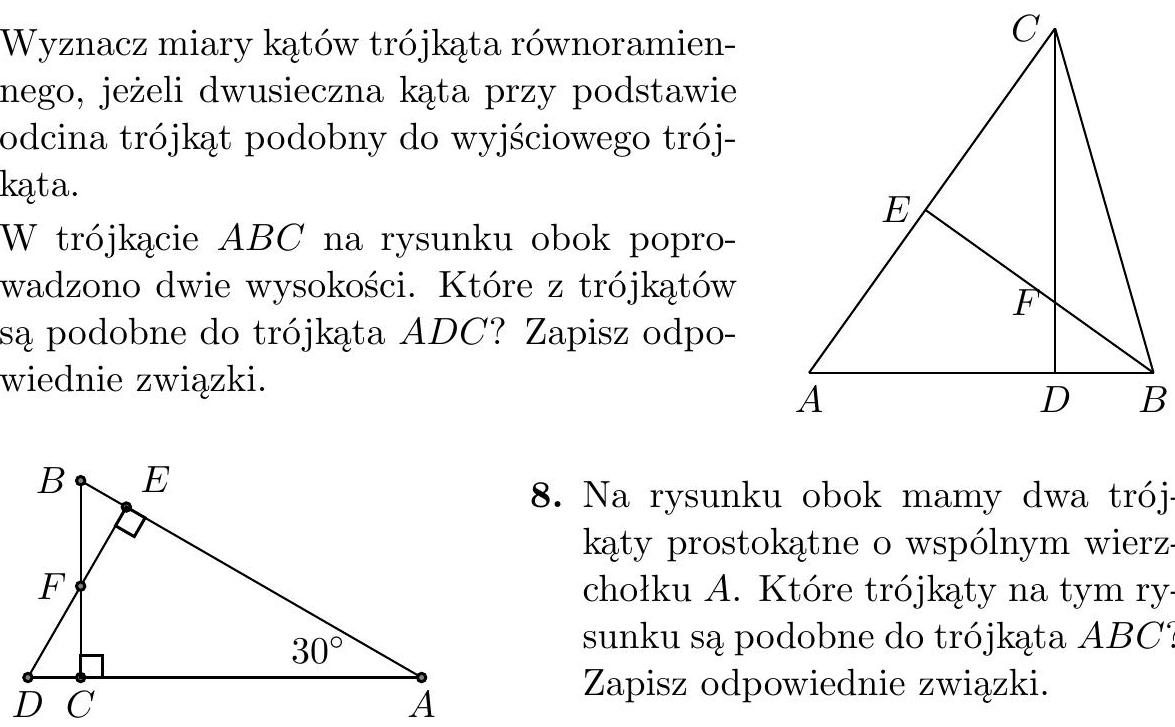
\includegraphics[max width=\textwidth, center]{2024_11_21_e9b4faa005d5be2cc318g-022(2)}
  \item Na rysunku obok mamy dwa trójkąty prostokątne o wspólnym wierzchołku \(A\). Które trójkąty na tym rysunku są podobne do trójkąta \(A B C\) ? Zapisz odpowiednie związki.
  \item Na rysunku obok boki trójkąta \(A B C\) połączono odcinkami \(D E\) i \(D F\) tak, że \(\Varangle A B C=\Varangle D E C\) i \(\Varangle B A C=\Varangle D F C\). Wskaż wszystkie pary trójkątów podobnych występujących na tym rysunku, zapisując odpowiednie związki.\\
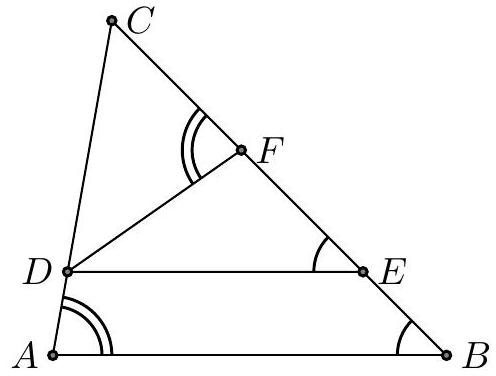
\includegraphics[max width=\textwidth, center]{2024_11_21_e9b4faa005d5be2cc318g-022(1)}
  \item W trójkącie równoramiennym kąt przy wierzchołku ma \(36^{\circ}\). Uzasadnij, że dwusieczna kąta przy podstawie dzieli ten trójkąt na dwa trójkąty równoramienne, przy czym jeden z nich jest podobny do wyjściowego trójkąta.
  \item W trójkącie ostrokątnym \(A B C\) poprowadzono wysokości \(A D, B E\) i \(C F\), które przecinają się w punkcie \(O\). Sporządź rysunek, wskaż wszystkie pary trójkątów podobnych zapisując odpowiednie związki.
  \item Dane jest koło \(k(O, r)\) i punkt \(P\) należący do wnętrza koła. Przez punkt \(P\) prowadzimy średnicę \(A B\) i dowolną cięciwę \(C D\). Wykaż, że \(\triangle A P C \sim \triangle B P D\).
  \item W trójkącie \(A B C\) wpisanym w okrąg dwusieczna kąta \(C\) przecina bok \(A B\) w punkcie \(D\), zaś okrąg, w punkcie \(E\). Pokaż, że \(\triangle C D B \sim\) \(\triangle A D E \sim \triangle C A E\). Jaka jest druga trójka trójkątów podobnych? Zapisz odpowiednie związki.\\
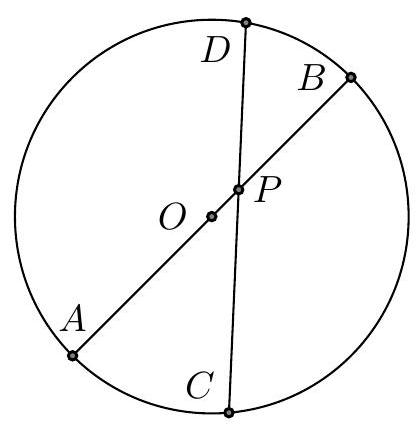
\includegraphics[max width=\textwidth, center]{2024_11_21_e9b4faa005d5be2cc318g-023}
  \item Dany jest okrąg i punkt \(P\) na zewnątrz tego okręgu. Przez punkt \(P\) prowadzimy dwie proste: jedną przez środek okręgu, która przecina go kolejno w punktach \(A\) i \(B\), drugą przecinającą go kolejno w punktach \(C\) i \(D\). Pokaż, że \(\triangle P B C \sim \triangle P D A\) i \(\triangle P A C \sim \triangle P D B\).
\end{enumerate}

Obecnie sformułujemy dwa twierdzenia, które pozwalają rozstrzygnąć, czy dane dwa trójkąty są podobne. Są to tzw. cechy podobieństwa trójkątów.\\
CECHA BKB\\
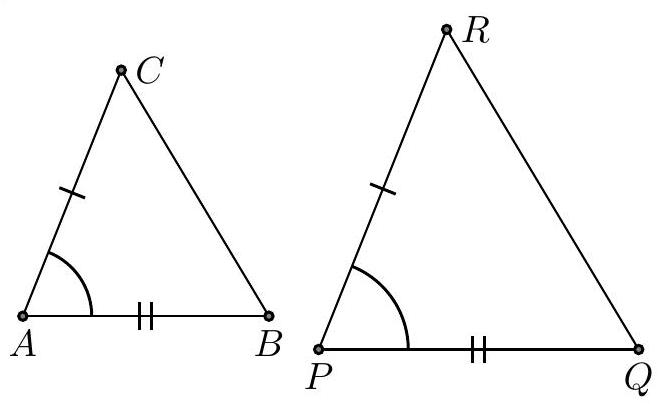
\includegraphics[max width=\textwidth, center]{2024_11_21_e9b4faa005d5be2cc318g-023(1)}

Jeżeli dla trójkątów \(A B C\) i \(P Q R\)\\
zachodzą równości: \(\frac{A C}{P R}=\frac{A B}{P Q}\) oraz \(\Varangle C A B=\Varangle R P Q\), to \(\triangle A B C \sim \triangle P Q R\).\\
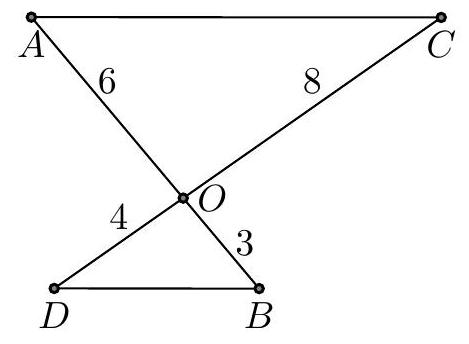
\includegraphics[max width=\textwidth, center]{2024_11_21_e9b4faa005d5be2cc318g-023(2)}\\
15. Na rysunku obok proste \(A B\) i \(C D\) przecinają się w punkcie \(O\). Na podstawie cechy BKB podobieństwa oraz długości podanych odcinków uzasadnij, że trójkąty \(A C O\) i \(B D O\) są podobne. Uzasadnij następnie, że \(\overline{A C} \| \overline{B D}\).\\
16. Na podstawie cechy \(\mathbf{B K B}\) podobieństwa trójkątów uzasadnij, że trójkąt \(A B C\) jest podobny do zacieniowanego trójkąta \(B D E\). Zapisz odpowiedni związek. Na rysunku zaznaczaj odpowiadające sobie kąty taką samą ilością łuków. Pod rysunkiem wpisz skalę podobieństwa (większego do mniejszego).\\
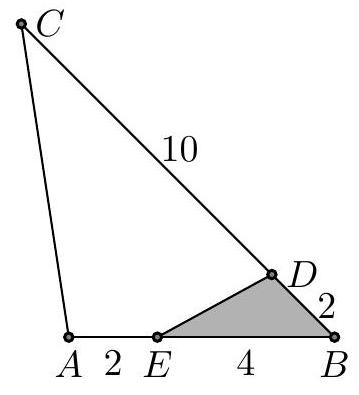
\includegraphics[max width=\textwidth, center]{2024_11_21_e9b4faa005d5be2cc318g-024(1)}\\
\(\lambda=\) \(\qquad\)\\
\(\qquad\)\\
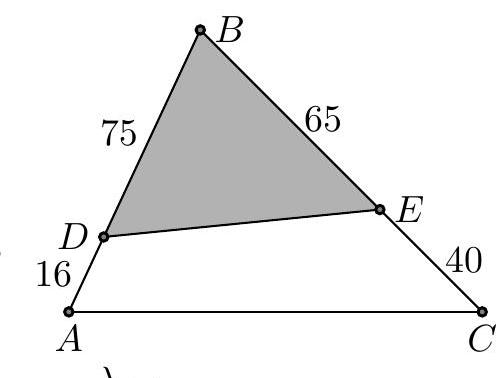
\includegraphics[max width=\textwidth, center]{2024_11_21_e9b4faa005d5be2cc318g-024}\\
\(\lambda=\) \(\qquad\)\\
17. Na rysunku obok proste \(A B\) i \(C D\) przecinają się w punkcie \(O\). Na podstawie cechy BKB oraz długości podanych odcinków rozstrzygnij czy a) \(\overline{A C} \| \overline{B D}\), b) \(\overline{E F} \| \overline{A C}\).\\
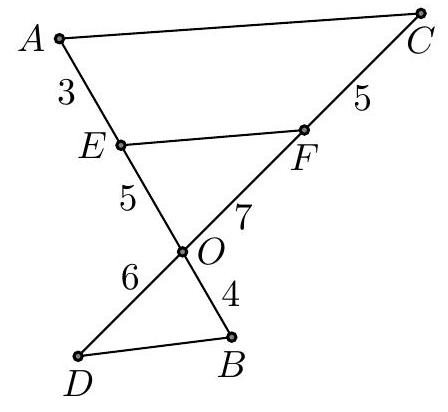
\includegraphics[max width=\textwidth, center]{2024_11_21_e9b4faa005d5be2cc318g-024(3)}

\section*{CECHA BBB}
\begin{center}
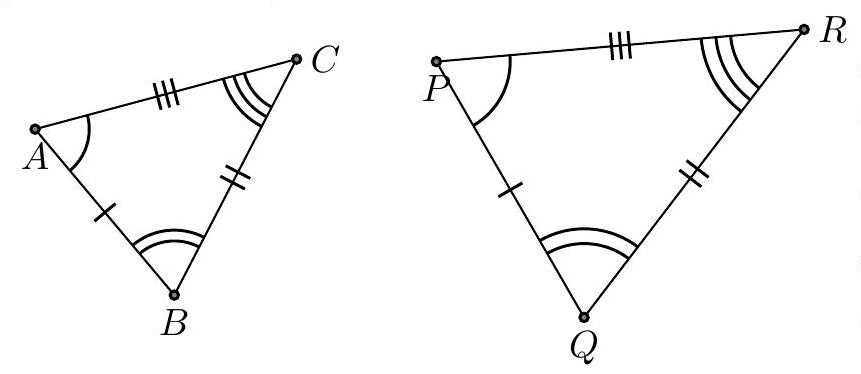
\includegraphics[max width=\textwidth]{2024_11_21_e9b4faa005d5be2cc318g-024(2)}
\end{center}

Jeżeli dla trójkątów \(A B C\) i \(P Q R\) zachodzi \(\frac{A B}{P Q}=\frac{B C}{Q R}=\frac{A C}{P R}\),\\
to\\
\(\triangle A B C \sim \triangle P Q R\).\\
Innymi słowy: jeżeli w dwóch trójkątach ilorazy długości boków jednego trójkąta przez długości odpowiadających im boków drugiego trójkąta są równe, to te trójkąty są podobne.\\
18. Dany jest trójkąt \(A B C\). Punkty \(P, Q\) i \(R\) są środkami boków \(A B, B C\) i \(C A\) odpowiednio. Pokaż, że \(\triangle A B C \sim \triangle Q R P\).\\
19. W trójkącie prostokątnym \(A B C\) kąt \(C\) jest prosty, zaś \(A C=3, B C=4\). W trójkącie \(P Q R\) kąt \(R\) jest prosty, zaś \(P Q=25, P R=15\). Korzystając z cechy BBB podobieństwa trójkątów, uzasadnij, że trójkąty \(A B C\) i \(P Q R\) są podobne. Zapisz odpowiedni związek.

Obecnie sformułujemy trzy twierdzenia, które mówią nam jakie własności mają trójkąty podobne. Jedna z tych własności jest podstawą określenia tzw. funkcji trygonometrycznych.

\section*{TWIERDZENIE 1}
Jeżeli \(\triangle A B C \sim \triangle P Q R\), to wówczas

\begin{enumerate}
  \item \(\frac{A B}{P Q}=\frac{B C}{Q R} \quad\) czyli \(\quad \frac{A B}{B C}=\frac{P Q}{Q R} \quad\) czyli \(A B \cdot Q R=B C \cdot P Q\),
  \item \(\Varangle A B C=\Varangle P Q R\).
\end{enumerate}

Zauważmy, że jest to odwrócenie cechy BKB podobieństwa trójkątów.\\
Prawdziwe jest również twierdzenie odwrotne do cechy \(\mathbf{B B B}\) a mianowicie

\section*{TWIERDZENIE 2}
Jeżeli \(\triangle A B C \sim \triangle P Q R\), to \(\frac{A B}{P Q}=\frac{B C}{Q R}=\frac{A C}{P R}\).\\
Twierdzenie to mówi, że stosunek długości odpowiadających sobie boków w dwóch trójkątach podobnych jest stały. Nazywamy go skalą podobieństwa tych trójkątów i oznaczamy zazwyczaj literą \(\lambda\) lub \(k\).

\section*{TWIERDZENIE 3}
Jeżeli \(\triangle A B C \sim \triangle P Q R \quad\) i \(\quad \frac{A B}{P Q}=\lambda\), to stosunek długości jakichkolwiek dwóch odpowiadających sobie elementów w trójkątach \(A B C\) i \(P Q R\) jest równy \(\lambda\). Liczbę \(\lambda\) nazywamy skala podobieństwa tych trójkatów.\\
PRZYKŁAD\\
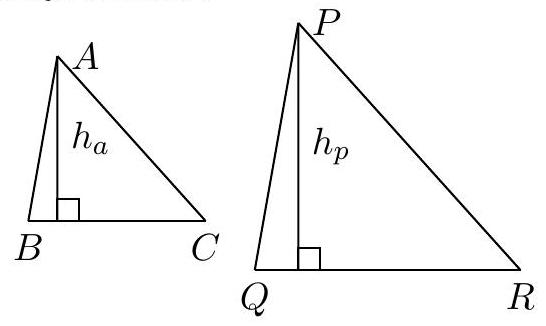
\includegraphics[max width=\textwidth, center]{2024_11_21_e9b4faa005d5be2cc318g-025}

Na rysunku obok \(\triangle A B C \sim \triangle P Q R\), przy czym \(\frac{A B}{P Q}=\frac{B C}{Q R}=\frac{A C}{P R}=\lambda\), wobec tego \(\frac{h_{a}}{h_{p}}=\lambda\), gdzie \(h_{a}\) i \(h_{p}\) są to wysokości wychodzące odpowiednio z wierzchołków \(A\) i \(P\).\\
20. Cięciwy \(A B\) i \(C D\) okręgu przecinają się w punkcie \(P\). Wykaż, że \(|P B| \cdot|P A|=|P C| \cdot|P D|\), czyli, że \(\frac{|P B|}{|P C|}=\frac{|P D|}{|P A|}\).\\
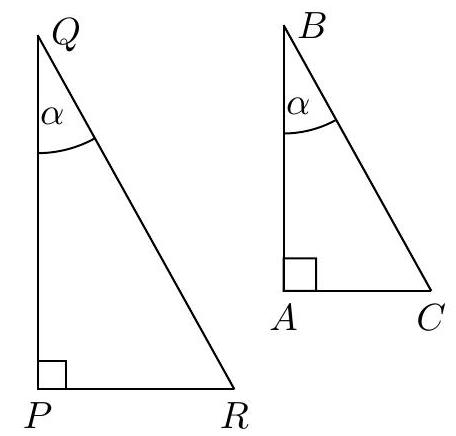
\includegraphics[max width=\textwidth, center]{2024_11_21_e9b4faa005d5be2cc318g-026(1)}\\
21. Trójkąty prostokątne \(A B C\) i \(P Q R\) na rysunku obok są podobne. Wiedząc, że \(|B A|=4,|A C|=3,|P R|=12\), wyznacz \(|P Q|\) i \(|Q R|\).\\
22. Cięciwy \(A B\) i \(C D\) okręgu przecinają się w punkcie \(P\). Wiedząc, że \(|A B|=42\), \(|A P|:|P B|=3: 4\) i \(|C P|:|P D|=1: 3\), oblicz długość odcinka \(C D\).

23* W trójkącie równobocznym \(A B C\) przez punkt przecięcia środkowych poprowadzono prostą równoległą do boku \(A B\). W jakim stosunku dzieli ona boki \(A C\) i \(B C\) ?\\
24. Przekątne \(A C\) i \(B D\) trapezu \(A B C D\) przecinają się w punkcie \(S \mathrm{w}\) ten sposób, że \(|A S|:|A C|=3: 4\). Wyznacz \(|C D|\) jeżeli \(|A B|=12\).\\
25. Proste \(k\) i \(l\) na rysunku obok są równoległe. Wskaż równe kąty w obu trójkątach. Wyznacz długość odcinka \(x\).\\
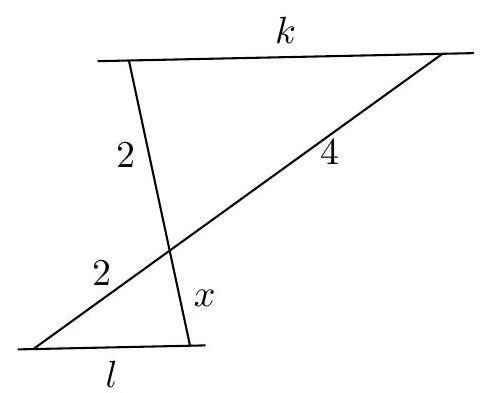
\includegraphics[max width=\textwidth, center]{2024_11_21_e9b4faa005d5be2cc318g-026(2)}\\
26. (matura 2016) Uzasadnij, że trój-\\
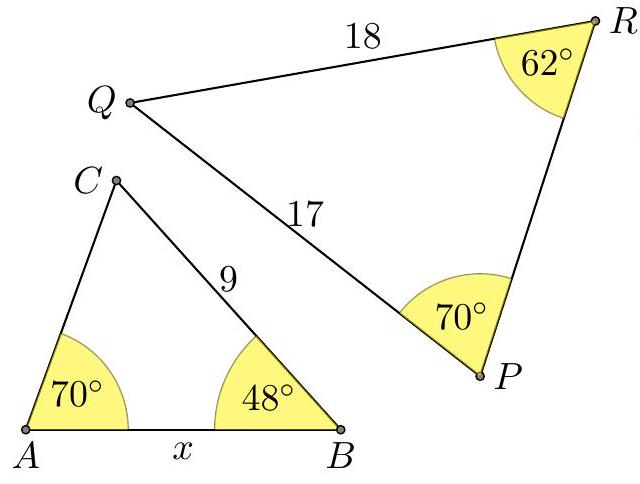
\includegraphics[max width=\textwidth, center]{2024_11_21_e9b4faa005d5be2cc318g-026}\\
kąty \(A B C\) i \(P Q R\) są podobne. Wyznacz długość odcinka \(A B\).\\
27. Punkt \(P\) leży na zewnątrz okręgu. Prowadzimy przez ten punkt dwie proste. Jedna z nich przechodzi przez środek okręgu i przecina okrąg kolejno w punktach \(A, B\), a druga przecina okrąg kolejno w punktach \(C, D\). Uzasadnij, że \(|P A| \cdot|P B|=|P C| \cdot|P D|\).

28* W trójkącie ostrokątnym \(A B C\) poprowadzono wysokości \(A A_{1}\) i \(B B_{1}\). Pokaż, że \(A_{1} C \cdot B C=B_{1} C \cdot A C\), tym samym \(\triangle A B C \sim \triangle A_{1} B_{1} C\).\\
29. Dane są trójkąty \(A B C\) i \(A^{\prime} B^{\prime} C^{\prime}\), przy czym \(\triangle A B C \sim \triangle A^{\prime} B^{\prime} C^{\prime}\). Długości boków trójkąta \(A B C\) są równe \(36,63,81\). Obwód trójkąta \(A^{\prime} B^{\prime} C^{\prime}\) jest równy 140. Wyznacz skalę podobieństwa tych trójkątów oraz boki trójkąta \(A^{\prime} B^{\prime} C^{\prime}\).\\
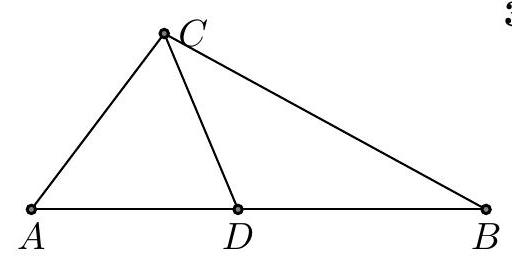
\includegraphics[max width=\textwidth, center]{2024_11_21_e9b4faa005d5be2cc318g-027}\\
30. Trójkąty \(A B C\) i \(C B D\) na rysunku obok są podobne, przy czym \(\triangle A B C \sim\) \(\triangle C B D\). Boki trójkąta \(C B D\) mają długości \(|C D|=2,|D B|=3,|B C|=4\). Znajdź długości boków \(A B\) i \(A C\). Jaka jest skala podobieństwa tych trójkątów?\\
31. W trapezie \(A B C D\) o podstawach \(A B\) i \(C D\) przekątne \(A C\) i \(B D\) przecinają się w punkcie \(O,|A B|=9,|C D|=6\). Wyznacz skalę podobieństwa trójkątów \(A B O\) i \(C D O\).\\
32. Podstawy trapezu mają długości odpowiednio 9 i 15 , a jego wysokość ma długość 12. Wyznacz odległość punktu przecięcia przekątnych tego trapezu od jednej i drugiej podstawy.

33* W trójkącie prostokątnym \(A B C\) kąt \(C\) jest prosty, \(|A C|=15 \mathrm{i}|B C|=20\). Wysokość \(C D\) podzieliła trójkąt \(A B C\) na dwa trójkąty \(A C D\) i \(B C D\). Każde dwa z tych trzech trójkątów są podobne. Wyznacz skalę podobieństwa dla każdej z tych trzech par trójkątów.\\
34. Podstawa \(A B\) trójkąta \(A B C\) ma długość 10. Punkty \(D\) i \(E\) leżą na ramionach trójkąta, przy czym \(\overline{A B} \| \overline{D E}\). Wysokość trójkąta \(C D E\) wychodząca z wierzchołka \(C\) ma długość 3 , zaś wysokość trapezu jest równa 5. Wyznacz \(P_{A B D E}\).\\
35. W trapezie \(A B C D\) podstawa \(A B\) ma długość 12 , a podstawa \(C D\) długość 8. Wysokość trapezu ma długość 6. Przekątne trapezu przecinają się w punkcie \(O\). Wyznacz skalę podobieństwa trójkątów \(A B O\) i \(C D O\). Oblicz odległość punktu przecięcia przekątnych tego trapezu od podstaw.

36* W trapezie prostokątnym podstawy mają długości 12 i 4 . Wysokość tego trapezu wynosi 6 . Wyznacz odległość punktu, w którym przecinają się przekątne trapezu, od obu podstaw i od obu ramion.\\
37. Punkt \(M\) jest środkiem boku \(C D\) równoległoboku \(A B C D\). Zbadaj jaką część pola równoległoboku stanowi pole trójkąta \(A B N\).\\
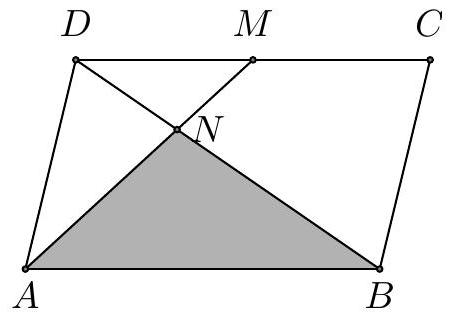
\includegraphics[max width=\textwidth, center]{2024_11_21_e9b4faa005d5be2cc318g-027(1)}\\
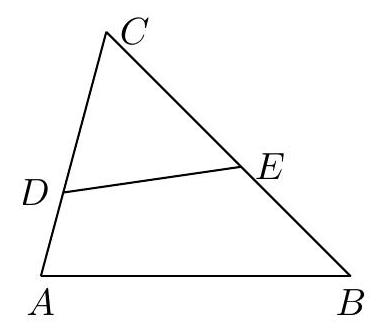
\includegraphics[max width=\textwidth, center]{2024_11_21_e9b4faa005d5be2cc318g-028(1)}\\
38. Na rysunku obok \(\triangle A B C \sim \triangle E D C\). Wiedząc, że \(|A B|=9,|A D|=2,|D C|=6\), \(|C E|=5\), wyznacz \(|B E|\) i \(|D E|\). Wyznacz skalę podobieństwa tych trójkątów.\\
39. W równoległoboku \(A B C D\) kąty \(\Varangle B\) i \(\Varangle D\) są rozwarte. Na prostych \(B C\) i \(C D\) obrano odpowiednio punkty \(M\) i \(N\) będące rzutami prostopadłymi punktu \(A\) na te proste. Pokaż, że \(\Varangle A B C=\Varangle M A N\) i \(\triangle M A N \sim \triangle A B C\).\\
40. W trójkąt \(A B C\) wpisano kwadrat \(P Q R S\) tak, że wierzchołki \(P\) i \(Q\) leżą na bokach \(A B\) i \(A C\), a wierzchołki \(R\) i \(S\) na boku \(B C\). Wyznacz długość boku kwadratu w zależności od \(a\) i \(h\), gdzie \(h\) oznacza wysokość wychodzącą z wierzchołka \(A\), zaś \(a\) oznacza długość boku \(B C\).\\
41. W trójkącie prostokątnym \(A B C\) kąt \(C\) jest prosty, punkt \(N\) leży na boku \(A B\), przy czym, \(\overline{C N} \perp \overline{A B}\). Oznaczmy długości poszczególnych odcinków: \(A C=b, B C=a, C N=h, A N=d, B N=e, A B=c\). Pokaż, że \(b^{2}=c d, a^{2}=c e, h^{2}=d e\).\\
\includegraphics[max width=\textwidth, center]{2024_11_21_e9b4faa005d5be2cc318g-028}

\section*{Dowód:}
Oznaczmy \(B C=a, A A^{\prime}=h_{a}\), wówczas \(Q R=\lambda a, P P^{\prime}=\lambda h_{a}\). Mamy wówczas \(P_{A B C}=\frac{1}{2} a h\), zaś \(P_{P Q R}=\frac{1}{2} \lambda a \cdot \lambda h_{a}=\lambda^{2} \cdot \frac{1}{2} a h=\lambda^{2} \cdot P_{A B C}\).\\
42. W trapezie \(A B C D\) podstawa \(A B\) ma długość 3 , a podstawa \(C D\) ma długość 2. Przekątne \(A C\) i \(B D\) przecinają się w punkcie \(E\). Wyznacz stosunek pól trójkątów \(A B E\) i \(C D E\),\\
43. Skala podobieństwa trójkąta \(A B C\) do trójkąta \(X Y Z\) jest równa \(2 \frac{1}{2}: 1\) (czyli \(\lambda=\frac{5}{2}\) ) Pole trójkąta \(X Y Z\) jest równe 50. Wyznacz pole trójkąta \(A B C\).\\
44. Trójkąt \(A B C\) jest podobny do trójkąta \(X Y Z\). Pole trójkąta \(A B C\) jest równe \(12 \frac{1}{2}\), a pole trójkąta \(X Y Z\) jest równe 32 . Najdłuższy bok w trójkącie \(A B C\) jest równy 5. Jaka jest skala podobieństwa tych trójkątów? Jaka jest wobec tego długość najdłuższego boku w trójkącie \(X Y Z\).\\
45. Trójkąty \(A B C\) i \(X Y Z\) są podobne. Najkrótszy bok w trójkącie \(A B C\) ma długość 6, a w trójkącie \(X Y Z 15\). Pole trójkąta \(A B C\) jest równe 12. Wyznacz pole trójkąta \(X Y Z\).\\
46. Patryk porównał dwa plany swojej miejscowości. Jeden z nich był sporządzony w skali 1:5000, a drugi 1:20 000. Na pierwszym odległość mierzona w linii prostej między budką telefoniczną koło jego szkoły a przystankiem autobusowym przy przy jego domu jest o \(4,5 \mathrm{~cm}\) większa, niż na drugim planie. Jak jest rzeczywista odległość w linii prostej między tymi miejscami?\\
47. Działka budowlana o powierzchni 16 arów na planie ma powierzchnię \(1,6 \cdot 10^{-3} \mathrm{~m}^{2}\). Jaka jest skala tego planu?\\
48. Prostokąt \(P_{1}\) ma pole \(5 \mathrm{~cm}^{2} \mathrm{i}\) jest podobny do prostokąta \(P\). Prostokąt \(P\) ma wymiary 5 cm i 9 cm . Jaka jest skala podobieństwa prostokąta \(P_{1}\) do \(P\) ?\\
49. Przez punkt \(D\) leżący na boku \(A C\) trójkąta \(A B C\) poprowadzono proste \(D E\) i \(D F, E \in \overline{A B}, F \in \overline{B C}\). równoległe do pozostałych boków trójkąta. Pole trójkąta \(A E D\) wynosi 1, a pole trójkąta \(C D F\) jest równe 4. Znajdź pole trójkąta \(A B C\).\\
50. W trapezie \(A B C D\) podstawa \(A B\) ma długość \(a\), podstawa \(C D\) ma długość \(b\). Przekątne \(A C\) i \(B D\) przecinają się w punkcie \(O\). Wyznacz skalę podobieństwa trójkątów \(A B O\) i \(C D O\).\\
51. Przez punkt przecięcia przekątnych trapezu prowadzimy prostą równoległą do jego podstaw. Prosta ta przecina ramiona trapezu w punktach \(E\) i \(F\). Znajdź długość odcinka \(E F\), wiedząc, że podstawy trapezu mają długości \(a\) i \(b\).\\
52. W trapezie \(A B C D\) podstawa \(A B\) ma długość 3 , a podstawa \(C D\) ma długość 2. Przekątne \(A C\) i \(B D\) przecinają się w punkcie \(E\). Wyznacz stosunek pól trójkątów\\
a) \(\triangle A B E\) i \(\triangle C D E\),\\
b) \(\triangle A E D\) i \(\triangle A B E\).

\section*{DEFINICJA}
Dwa wielokąty nazywamy podobnymi jeżeli odpowiadające sobie kąty w tych wielokątach są równe, a stosunek długości odpowiadających sobie boków jest równy stałej wielkości \(\lambda\). Liczbę \(\lambda\) nazywamy skala podobieństwa tych wielokatów.

TWIERDZENIE 5 (o wielokątach podobnych)\\
Jeżeli dwa wielokąty, na przykład pięciokąty \(A B C D E\) i \(P Q R S T\) są podobne i ich skala podobieństwa jest równa \(\lambda\), tzn. \(\frac{P Q}{A B}=\frac{Q R}{B C}=\frac{R S}{C D}=\frac{S T}{D E}=\) \(\frac{P T}{A E}=\lambda\), to wówczas

\begin{enumerate}
  \item stosunek dwóch odpowiadających sobie wielkości w tych wielokątach jest równy \(\lambda\),
  \item \(P_{P Q R S T}=\lambda^{2} P_{A B C D E}\).
\end{enumerate}

\section*{Wskazówki i odpowiedzi.}
\begin{enumerate}
  \item \(\triangle A C D \sim \triangle A B C \sim \triangle C B D\)
  \item \(\triangle A B C \sim \triangle Q R P\)
  \item kąty przy podstawie maja po \(72^{\circ}\), kąt przy wierzchołku ma \(36^{\circ}\)
  \item \(\triangle A D C \sim \triangle A E B \sim \triangle F D B \sim \triangle F E C\)
  \item \(\triangle A B C \sim \triangle A D E \sim \triangle F D C \sim F B E\)
  \item \(\triangle A B C \sim \triangle D E C \sim \triangle F D C\)
  \item \(\triangle B A E \sim \triangle B O F \sim \triangle C O E \sim \triangle C A F\),\\
\(\triangle C B F \sim \triangle C O D \sim \triangle A O F \sim \triangle A B D\),\\
\(\triangle A O E \sim \triangle A C D \sim \triangle B O D \sim \triangle B C E\).
  \item \(\triangle C A D \sim \triangle B E D \sim \triangle C E B\)
  \item a) \(\frac{E B}{B C}=\frac{D B}{A B}=\frac{1}{3}, \triangle E B D \sim \triangle A B C, \lambda=3\)\\
b) \(\frac{B E}{B C}=\frac{D B}{A B}=\frac{1}{2}, \triangle B E D \sim \triangle A C B, \lambda=2\)\\
c) \(\triangle A B C \sim \triangle E B D, \lambda=\frac{7}{5}\)
  \item a) tak, b) nie
  \item \(\frac{P R}{A C}=\frac{R Q}{C B}=\frac{P Q}{A B}=5\) zatem \(\triangle A B C \sim \triangle P Q R\)
  \item \(|P Q|=16,|Q R|=20\)
  \item \(|C D|=48\)
  \item wsk. co trzeba dorysować? 1 : 2
  \item \(|C D|=4\)
  \item \(x=1\).
  \item \(A B=8 \frac{1}{2}\)
  \item \(\lambda=\frac{9}{7},\left|A^{\prime} B^{\prime}\right|=28,\left|B^{\prime} C^{\prime}\right|=49,\left|A^{\prime} C^{\prime}\right|=63\)
  \item \(|A B|=\frac{16}{3},|A C|=\frac{8}{3}, \lambda=\frac{3}{4}\).
  \item \(\lambda=\frac{3}{2}\)
  \item \(d_{1}=4 \frac{1}{2}, d_{2}=7 \frac{1}{2}\)
  \item \(\triangle A B C / \triangle C B D=\frac{5}{4}, \triangle A B C / \triangle C D A=\frac{5}{3}, \triangle C B D / \triangle C D A=\frac{4}{3}\)
  \item \(P_{A B D E}=34 \frac{3}{8}\)
  \item \(\lambda=\frac{3}{2}, d_{1}=2 \frac{2}{5}, d_{2}=3 \frac{3}{5}\)
  \item od podstaw \(1 \frac{1}{2}, 4 \frac{1}{2}\), od ramion \(3, \frac{9}{5}\)
  \item \(P_{A B N}=\frac{1}{3} P_{A B C D}\)
  \item \(|B E|=\frac{23}{5},|D E|=\frac{45}{8}, \lambda=\frac{8}{5}\)
  \item \(|P Q|=\frac{a h}{a+h}\)
  \item \(\frac{9}{4}\)
  \item \(P_{A B C}=8\)
  \item \(\lambda=\frac{8}{5}\), najdłuższy bok w tr. \(X Y Z\) ma długość 8 .
  \item \(P_{X Y Z}=75\)
  \item 300 m
  \item \(\lambda=1: 1000\)
  \item \(\lambda=3\)
  \item \(P=9\),
  \item \(\lambda=\frac{a}{b}\)
  \item \(\frac{2 a b}{a+b}\)
  \item a) \(\frac{9}{4}\), b) \(\frac{2}{3}\)
\end{enumerate}

\section*{Rozdział 3}
\section*{STYCZNA DO OKREGGU}
DEFINICJA Jeżeli prosta i okrąg mają dokładnie jeden punkt wspólny, to tę prostą nazywamy styczna do okręgu, a ich jedyny punkt wspólny nazywamy punktem styczności. Odcinek łączący środek okręgu z dowolnym punktem okręgu nazywamy promieniem.\\
\includegraphics[max width=\textwidth, center]{2024_11_21_e9b4faa005d5be2cc318g-032(1)}

Posługując się pojęciem stycznej do okręgu będziemy wielokrotnie korzystać nie z definicji stycznej tylko z jej własności, które wynikają z definicji. Własności te wyrażamy zazwyczaj w postaci następujących dwóch twierdzeń:\\
\includegraphics[max width=\textwidth, center]{2024_11_21_e9b4faa005d5be2cc318g-032}

TWIERDZENIE Jeżeli prosta \(k\) jest styczna do okręgu, to jest ona prostopadła do promienia tego okręgu wychodzącego z punktu styczności.

TWIERDZENIE Jeżeli prosta \(k\) jest prostopadła do promienia \(O A\) w okręgu o środku w punkcie \(O\) i przechodzi przez punkt \(A\) leżący na tym okręgu, to jest ona styczna do tego okręgu.

\begin{enumerate}
  \item Prosta \(M P\) jest styczna do okręgu \(\mathcal{K}(O, 7)\) w punkcie \(P\). Odległość od punktu \(M\) do punktu \(O\) wynosi 25 . Wyznacz \(|M P|\).
  \item Punkt \(A\) leży na zewnątrz okręgu \(\mathcal{K}(C, 15)\). Prosta \(A B\) jest styczna do tego okręgu w punkcie \(B . P_{A B C}=150\). Wyznacz \(|A B| \mathrm{i}|A C|\).
  \item Niech prosta \(l\) przechodząca przez punkt \(M\) będzie styczna do okręgu \(\mathcal{K}(O, 10)\) w punkcie \(P\) i niech \(|M P|=24\). Półprosta \(M O\) przecina ten okrąg kolejno w punktach \(Q\) i \(R\). Wyznacz \(|M R|\).
  \item Prosta \(l\) przechodząca przez punkt \(M\) jest styczna do okręgu \(\mathcal{K}(O, 4) \mathrm{w}\) punkcie \(P\), zaś prosta \(M O\) przecina okrąg \(\mathcal{K}\) kolejno w punktach \(Q\) i \(R\). Odcinek \(M P\) jest o 3 dłuższy od odcinka \(M Q\). Wyznacz kolejno:\\
a) \(M P\), b) \(P_{M O P}\), c) \(d\left(P, l_{M O}\right)\).\\
\includegraphics[max width=\textwidth, center]{2024_11_21_e9b4faa005d5be2cc318g-033}
  \item Na rysunku obok mamy dwa półokręgi o wspólnym środku \(O\). Promień mniejszego półokręgu ma długość 3, a większego 5. Proste \(L M\) i \(P I\) są styczne do mniejszego półokręgu. Wyznacz \(|L M|\) i \(|P I|\).
  \item Dane są dwa okręgi współśrodkowe o promieniach 15 i 9. Jaka jest długość cięciwy większego okręgu, która jest styczna do mniejszego okręgu.
  \item Dany jest kąt prosty o wierzchołku \(P\). Okrąg styczny w punkcie \(M\) do jednego ramienia tego kąta przecina drugie ramię w punktach \(A\) i \(B\). Oblicz promień tego okręgu wiedząc, że \(|P M|=24,|A B|=20\).
  \item Niech \(M\) będzie punktem leżącym na zewnątrz okręgu o środku w punkcie \(O\). Prosta \(l\) przechodzi przez punkt \(M\) i jest styczna do okręgu w punkcie \(P\). Druga prosta \(k\) przechodzi przez punkt \(M\) i przez środek okręgu. Przecina ona okrąg w punktach \(Q\) i \(R\). Pokaż, że \(|M P|^{2}=\) \(|M Q| \cdot|M R|\).
  \item Kąt utworzony przez dwa promienie okręgu wynosi \(130^{\circ}\). Wyznacz kąt ostry, który tworzą styczne poprowadzone przez końce promieni.
  \item Z punktu zewnętrznego \(A\) poprowadzono styczne \(A B\) i \(A C\) do okręgu o środku w punkcie \(O\), przy czym \(B\) i \(C\) są punktami styczności. Kąt pomiędzy stycznymi ma \(35^{\circ}\). Jaki jest kąt wypukły pomiędzy promieniami poprowadzonymi ze środka okręgu do punktów styczności?
  \item Do danego okręgu poprowadzono styczną tak, że końce \(A\) i \(B\) średnicy \(A B\) tego okręgu są odległe od stycznej o 25 cm i 15 cm . Wyznacz długość średnicy \(A B\).
  \item Niech \(l\) będzie prostą styczną do pewnego okręgu, a odcinek \(A B\) dowolną jego średnicą. Oznaczmy przez \(A^{\prime}\) i \(B^{\prime}\) rzuty prostokątne punktów \(A\) i \(B\) na prostą \(l\). Udowodnij, że \(|A B|=\left|A A^{\prime}\right|+\left|B B^{\prime}\right|\).\\
\includegraphics[max width=\textwidth, center]{2024_11_21_e9b4faa005d5be2cc318g-034}
  \item Proste \(A B\) i \(A C\) na rysunku obok są styczne do okręgu. Wyznacz miarę kąta \(B D C\).
  \item Na rysunku obok z punktu \(P\) wychodzą dwie proste styczne do okręgu w punktach \(A\) i \(B\). Punkt \(C\) leży na okręgu. Wyznacz \(\varepsilon\).\\
\includegraphics[max width=\textwidth, center]{2024_11_21_e9b4faa005d5be2cc318g-034(1)}
\end{enumerate}

DEFINICJA Okrąg styczny do wszystkich trzech boków trójkąta nazywamy okręgiem wpisanym (w ten trójkąt).\\
15. Okrąg na rysunku obok wpisany jest w trójkąt \(A B C\), przy czym \(D, E, F\) są punktami styczności, zaś punkt \(O\) jest środkiem okręgu. Wyznacz kolejno kąty \(x, y, z\).\\
\includegraphics[max width=\textwidth, center]{2024_11_21_e9b4faa005d5be2cc318g-034(2)}\\
16. Trójkąt \(A B C\) na rysunku obok jest opisany na okręgu. Punkty \(P, Q, M\) są punktami styczności. Wyznacz \(\gamma\) w zależności od \(\alpha\) i \(\beta\).

DEFINICJA Dwa okręgi nazywamy stycznymi gdy mają one dokładnie jeden punkt wspólny. Mają one wówczas wspólną styczną przechodzącą przez ich punkt styczności. Okręgi mogą być styczne zewnętrznie lub wewnętrznie.\\
\includegraphics[max width=\textwidth, center]{2024_11_21_e9b4faa005d5be2cc318g-035(1)}

Przykład pary okręgów zewnętrznie stycznych oraz pary okręgów wewnętrznie stycznych wraz z ich wspólną styczną.\\
\includegraphics[max width=\textwidth, center]{2024_11_21_e9b4faa005d5be2cc318g-035(2)}

TWIERDZENIE Jeżeli dwa okręgi są styczne zewnętrznie lub wewnętrznie, to ich środki oraz punkt styczności leżą na jednej prostej.\\
\includegraphics[max width=\textwidth, center]{2024_11_21_e9b4faa005d5be2cc318g-035}

WNIOSEK\\
Jeżeli okręgi \(\mathcal{K}\left(O_{1}, r_{1}\right)\) i \(\mathcal{K}\left(O_{2}, r_{2}\right)\) są zewnętrznie styczne, to

\[
\left|O_{1} O_{2}\right|=r_{1}+r_{2}
\]

zaś gdy są wewnętrznie styczne, to

\[
\left|O_{1} O_{2}\right|=\left\{\begin{array}{lll}
r_{1}-r_{2} & \text { gdy } & r_{1}>r_{2} \\
r_{2}-r_{1} & \text { gdy } & r_{2}>r_{1}
\end{array}\right.
\]

\begin{enumerate}
  \setcounter{enumi}{16}
  \item Trzy okręgi o promieniu 1 są styczne zewnętrznie, każdy do dwóch pozostałych. Wyznacz boki i kąty trójkąta utworzonego przez punkty styczności oraz pole trójkąta wyznaczonego przez środki okręgów.
  \item Środki trzech okręgów parami zewnętrznie stycznych są wierzchołkami trójkąta o bokach długości 3, 4, 5. Wyznacz długości promieni okręgów.
  \item Okręgi \(\mathcal{K}\left(B, r_{1}\right)\) i \(\mathcal{K}\left(C, r_{2}\right)\) są zewnętrznie styczne, a jednocześnie każdy z nich jest styczny wewnętrznie do okręgu \(\mathcal{K}\left(A, r_{3}\right)\). Oblicz długości promieni \(r_{1}, r_{2}\) i \(r_{3}\), wiedząc, że \(|A B|=4,|B C|=5\) i \(|A C|=3\).
  \item Okręgi \(\mathcal{K}_{1}\left(O_{1}, r_{1}\right)\) i \(\mathcal{K}_{2}\left(O_{2}, r_{2}\right)\) są styczne zewnętrznie, a równocześnie styczne wewnętrznie do okręgu \(\mathcal{K}_{3}\left(O_{3}, r_{3}\right)\). Obwód trójkąta \(O_{1} O_{2} O_{3}\) jest równy 26. Wyznacz \(r_{3}\).\\
\includegraphics[max width=\textwidth, center]{2024_11_21_e9b4faa005d5be2cc318g-036(1)}
  \item Okrąg o środku w punkcie \(A\) ma promień długości 3 , zaś styczny do niego okrąg o środku w punkcie \(B\) ma promień długości 12. Punkty \(P\) i \(Q\) leżą na okręgu i są punktami styczności. Wyznacz pole czworokata \(A P B Q\).
  \item Dany jest trapez o ramionach długości 24 i 32. Ramiona trapezu są średnicami okręgów, które są zewnętrznie styczne. Wyznacz sumę długości podstaw trapezu.
  \item Okręgi \(\mathcal{K}_{1}\) i \(\mathcal{K}_{2}\) o środkach \(S_{1}\) i \(S_{2}\) są styczne zewnętrznie w punkcie \(B\). Przez punkt \(B\) prowadzimy prostą \(l\), która przecina okrąg \(\mathcal{K}_{1} \mathrm{w}\) punkcie \(A\), zaś okrąg \(\mathcal{K}_{2}\) w punkcie \(C\), tak że \(\Varangle B C S_{2}=25^{\circ}\). Wyznacz miarę kąta \(A S_{1} B\). Co możesz powiedzieć o prostych \(C S_{2}\) i \(A S_{1}\) ?
  \item Trzy okręgi o promieniu \(r\) są styczne zewnętrznie, każdy do dwóch pozostałych. Wyznacz boki i kąty trójkąta utworzonego przez punkty styczności oraz pole trójkąta wyznaczonego przez środki okręgów.
\end{enumerate}

25* Dwa okręgi \(\mathcal{K}_{1}\) i \(\mathcal{K}_{2}\) o środkach \(S_{1}\) i \(S_{2}\) są styczne a) zewnętrznie b) wewnętrznie w punkcie \(B\). Przez punkt \(B\) prowadzimy prostą różną od prostej \(l_{S_{1} S_{2}}\), która przecina okrąg \(\mathcal{K}_{1}\) w punkcie \(A_{1}\), zaś okrąg \(\mathcal{K}_{2} \mathrm{w}\) punkcie \(A_{2}\). Uzasadnij, że \(\overline{A_{1} S_{1}} \| \overline{A_{2} S_{2}}\).\\
\includegraphics[max width=\textwidth, center]{2024_11_21_e9b4faa005d5be2cc318g-036}\\
26. (matura 2016) Okręgi \(k_{1}(A, 3)\) i \(k_{2}(B, 4)\) są styczne. Prosta \(A C\) jest styczna do okręgu \(k_{2}\) w punkcie \(C\), zaś \(D\) jest punktem wspólnym okręgu \(k_{1}\) i tej stycznej. Wyznacz \(C D\).\\
\includegraphics[max width=\textwidth, center]{2024_11_21_e9b4faa005d5be2cc318g-037}\\
27. Okręgi \(\mathcal{K}_{1}\) i \(\mathcal{K}_{2}\) na rysunku obok są styczne zewnętrznie w punkcie \(X\). Przez punkt \(X\) prowadzimy proste \(l\) i \(m\), które przecinają okręgi we wskazanych punktach. Wiadomo, że \(\Varangle X C D=52^{\circ}\). Wyznacz kolejno \(\Varangle X D S_{2}, \Varangle X B S_{1}, \Varangle B S_{1} X\), \(\Varangle B A X\). Co możesz powiedzieć o czworokącie \(A B C D\) ?\\
28. Okręgi \(\mathcal{K}_{1}\) i \(\mathcal{K}_{2}\) są styczne a) zewnętrznie b) wewnętrznie w punkcie \(X\). Przez punkt \(X\) prowadzimy proste \(m\) i \(n\). Prosta \(m\) przecina okragg \(\mathcal{K}_{1} \mathrm{w}\) punkcie \(A\), zaś okrąg \(\mathcal{K}_{2}\) w punkcie \(B\). Prosta \(n\) przecina \(\mathcal{K}_{1}\) w punkcie \(C\), zaś \(\mathcal{K}_{2}\) w punkcie \(D\). Pokaż, że\\
a) \(l_{A C} \| l_{B D}\);\\
b) trójkąty \(X A C\) i \(X B D\) mają takie same kąty.\\
29. Na rysunku obok okrąg \(k\) jest wewnętrznie styczny do większego okręgu. Punkt \(M\) jest środkiem większego okręgu, a punkt \(O\) - mniejszego. Odcinek \(S M\) jest średnicą okręgu \(k\), zaś \(S P\) jest dowolną cięciwą w zewnętrznym okręgu, \(R\) jest punktem przecięcia okręgu \(k\) i cięciwy \(S P\). Uzasadnij, że okrąg \(k\) dzieli cięciwę \(S P\) na połowy, czyli że \(|P R|=|S R|\).\\
\includegraphics[max width=\textwidth, center]{2024_11_21_e9b4faa005d5be2cc318g-037(1)}

Z twierdzenia o dwusiecznej kąta wypukłego wiemy, że punkt leży na dwusiecznej kąta wtedy i tylko wtedy gdy jest on równo odległy od obu ramion kąta. Z tego wynika następujące twierdzenie:

TWIERDZENIE Wszystkie trzy dwusieczne kątów trójkąta przecinają się w jednym punkcie. Punkt ten jest tak samo oddalony od każdego boku czyli jest środkiem okręgu wpisanego w ten trójkąt.\\
\includegraphics[max width=\textwidth, center]{2024_11_21_e9b4faa005d5be2cc318g-037(2)}\\
\includegraphics[max width=\textwidth, center]{2024_11_21_e9b4faa005d5be2cc318g-038(1)}

Zauważmy, że\\
\(|I Z|=|I X|\), bo punkt \(I\) leży na dwusiecznej kąta \(\Varangle C A B\)\\
\(|I X|=|I Y|\), bo punkt \(I\) leży na dwusiecznej kąta \(\Varangle A B C\)\\
z tych równości wynika, że\\
\(|I Z|=|I Y|\), a to oznacza, że punkt \(I\) leży na dwusiecznej kąta \(\Varangle A C B\). Czyli dwusieczne wszystkich trzech kątów trójkąta przecinają się w jednym punkcie. Z tego wynika, że odcinki \(I X, I Y, I Z\) są wysokościami trójkątów \(A B I, B C I, A C I\).\\
\includegraphics[max width=\textwidth, center]{2024_11_21_e9b4faa005d5be2cc318g-038}\\
30. Na rysunku obok dwie półproste wychodzące z wierzchołka \(A\) dzielą kąt \(A\) na trzy równe części. Podobnie dwie półproste wychodzące z wierzchołka \(B\) dzielą kąt \(B\) na trzy równe części. Natomiast wszystkie cztery półproste przecinając się tworzą czworokąt. Pokaż, że wskazana na rysunku przerywaną linią przekątna tego czworokąta jest dwusieczną kąta \(\Varangle A O B\) tzn, że \(\varphi=\psi\).\\
31. Punkt \(O\) jest wierzchołkiem kąta (wypukłego). Punkty \(B\) i \(C\) leżą na jednym ramieniu kąta, zaś punkty \(A\) i \(D\) na drugim ramieniu, przy czym \(|O B|=|O A|,|O C|=|O D|\). Niech \(E\) będzie punktem przecięcia prostych \(A C\) i \(B D\). Uzasadnij, że punkt \(E\) leży na dwusiecznej kąta \(O C D\).\\
32. Trójkąt \(A B C\) wpisany jest w okrąg, zaś punkt \(I\) jest środkiem okręgu wpisanego w trójkąt \(A B C\). Półprosta \(A I\) przecina okrąg w punkcie \(D\). Uzasadnij, że \(D B=D I=D C\).

TWIERDZENIE Pole trójkąta o bokach długości \(a, b, c\) i promieniu okręgu wpisanego długości \(r\) jest równe

\[
P=\underbrace{\frac{1}{2}(a+b+c)}_{\text {połowa obwodu }} \cdot r
\]

\includegraphics[max width=\textwidth, center]{2024_11_21_e9b4faa005d5be2cc318g-039}\\
czyli krótko mówiąc: pole trójkąta jest równe iloczynowi połowy obwodu tego trójkąta przez promień okręgu wpisanego w ten trójkąt.

\section*{Dowód}
Zauważ, że promienie łączące środek okręgu z punktami styczności są wysokościami w trójkątach \(B C I, C A I, A B I\) wychodzącymi z wierzchołka \(I \mathrm{w}\) każdym z trójkątów, i wobec tego

\[
\begin{aligned}
P_{A B C} & =P_{B C I}+P_{C A I}+P_{A B I} \\
& =\frac{1}{2} a r+\frac{1}{2} b r+\frac{1}{2} c r \\
& =\frac{1}{2}(a+b+c) \cdot r
\end{aligned}
\]

UWAGA bardzo często połowę obwodu trójkąta oznacza się literą \(p\), wówczas wzór na pole trójkąta zapisuje się krócej

\[
P=p \cdot r
\]

\begin{enumerate}
  \setcounter{enumi}{32}
  \item W trójkącie prostokątnym przyprostokątne mają długości 3 i 4. Wyznacz promień okręgu wpisanego w ten trójkąt.
  \item Dany jest trójkąt prostokątny \(A B C\). Punkt \(C\) jest wierzchołkiem kąta prostego, \(|A C|=3,|B C|=4\). Dwusieczna kąta \(B A C\) dzieli trójkąt \(A B C\) na dwa trójkąty: \(A C D\) i \(A B D\). Wyznacz promień okręgu wpisanego w trójkąt \(A C D\) i w trójkąt \(A D B\).
  \item W trójkąt równoboczny o boku długości \(2 \sqrt{3}\) wpisano okrąg. Wyznacz długość promienia tego okręgu.
  \item Wyznacz promień okręgu wpisanego w trójkąt równoramienny o podstawie \(2 d\) i ramieniu długości \(l\).
  \item W trójkąt równoboczny o boku długości a wpisano okrąg. Wyznacz długość promienia tego okręgu.
  \item Dany jest trójkąt równoramienny o ramionach długości 13 i podstawie długości 10. Wyznacz długość promienia okręgu wpisanego w ten trójkąt.
\end{enumerate}

39* Dany jest trójkąt prostokątny o przyprostokątnych długości 5 i 12. Okrąg \(\mathcal{K}(P, 1)\), jest styczny do obu przyprostokątnych. Wyznacz odległość punktu \(P\) od przeciwprostokątnej.\\
40. Okrąg \(\mathcal{K}(O, R)\) styczny jest do przyprostokątnych trójkąta prostokątnego \(A B C\). Długości przyprostokątnych są równe 6 i 8 . Punkt \(O\) leży na przeciwprostokątnej \(A B\) tego trójkąta. Wyznacz \(R\).

Ma miejsce następujące twierdzenie zwane zasadniczym twierdzeniem planimetrii

TWIERDZENIE Jeżeli punkt \(R\) leży poza okręgiem, to wówczas przez ten punkt przechodzą dokładnie dwie styczne do tego okręgu, a przy tym odcinki zawarte między punktem \(R\) a punktami styczności z okręgiem, są równej długości, (czyli trójkąt \(A R B\) jest równoramienny). Na rysunku obok tymi odcinkami są \(A R\) i \(B R\).\\
\includegraphics[max width=\textwidth, center]{2024_11_21_e9b4faa005d5be2cc318g-040}

\section*{Dowód:}
Zauważ, że trójkąty \(A R O\) i \(B R O\) są prostokątne. Mają one wspólną przeciwprostokątną \(R O\), mają tej samej długości przyprostokątne \(A O\) i \(B O\) bo są one promieniami tego okręgu. Wobec tego z twierdzenia Pitagorasa wynika, że pozostałe dwie przyprostokątne czyli \(R A\) i \(R B\) też są tej samej długości.\\
Dla wykorzystania tego twierdzenia wprowadzimy dodatkowe pojęcie, a mianowicie:\\
\includegraphics[max width=\textwidth, center]{2024_11_21_e9b4faa005d5be2cc318g-040(1)}

DEFINICJA Okrąg styczny do jednego z boków trójkąta oraz styczny do przedłużeń dwóch pozostałych boków nazywamy okregiem dopisanym do trójkąta.\\
41. Na rysunku obok wszystkie trzy proste są styczne do okręgu. Punkty \(A, B\) i \(C\) są punktami styczności, \(|R A|=7\). Powiedz jaki jest wobec tego obwód trójkąta QRS.\\
\includegraphics[max width=\textwidth, center]{2024_11_21_e9b4faa005d5be2cc318g-041}\\
42. Okrąg \(\mathcal{K}\) jest okręgiem dopisanym do trójkąta \(A B C\) stycznym w punkcie\\
\(!\Rightarrow \quad D \in \overline{A B}\). Pokaż, że długość odcinka od wierzchołka \(C\) do punktu styczności zawartego w przedłużeniu boku \(A C\) jest równa połowie obwodu tego trójkąta.\\
43. Wyznacz promień okręgu dopisanego do trójkąta równoramiennego prostokątnego o ramionach długości \(a\). Rozpatrz dwa przypadki.\\
44. W trójkącie prostokątnym jedna z przyprostokątnych ma długość 12, zaś promień okręgu wpisanego jest równy 2. Wyznacz długości pozostałych boków w tym trójkącie.\\
45. Boki trójkąta mają długości 13, 20 21. Policz na jakiej długości odcinki dzielą boki tego trójkąta punkty styczności okręgu wpisanego w ten trójkąt.\\
46. Okręgi \(\mathcal{K}_{1}\) o środku \(S_{1}\) i \(\mathcal{K}_{2}\) o środku \(S_{2}\) są zewnętrznie styczne w punkcie \(B\). Przez ten punkt przechodzi prosta \(t\) styczna do obu okręgów. Druga prosta \(s\) jest styczna do okręgu \(\mathcal{K}_{1}\) w punkcie \(P\) a do okręgu \(\mathcal{K}_{2}\) w punkcie Q. Pokaż, że\\
a) punkt \(A\) przecięcia obu stycznych dzieli odcinek \(P Q\) na połowy.\\
b) \(\Varangle P B Q=90^{\circ}\).\\
c) \(\Varangle S_{1} A S_{2}=90^{\circ}\).\\
47. Oznaczmy przez \(a\) i \(b\) długości przyprostokątnych w trójkącie prostokątnym zaś przez \(c\) długość przeciwprostokątnej. Pokaż, że wówczas promień okręgu wpi\(!\Rightarrow \quad\) sanego w ten trójkąt ma długość

\[
r=\frac{a+b-c}{2}
\]

Spójrz na rysunek i napisz odpowiednią równość.\\
\includegraphics[max width=\textwidth, center]{2024_11_21_e9b4faa005d5be2cc318g-041(1)}\\
48. W trójkącie prostokątnym suma długości przyprostokątnych równa jest \(\sqrt{18}\), a przeciwprostokątna ma długość 4 . Oblicz promień okręgu wpisanego w ten trójkąt oraz pole trójkąta .\\
49. Przekątne w rombie mają długości 8 i 6 . Dzielą one romb na cztery trójkąty prostokątne. Oblicz pole czworokąta, którego wierzchołkami są środki okręgów wpisanych w te cztery trójkąty.\\
50. W trójkącie prostokątnym wpisanym w okrąg o średnicy \(5 \sqrt{5}\) jedna z przyprostokątnych jest 2 razy dłuższa od drugiej przyprostokątnej. Oblicz promień okręgu wpisanego w ten trójkąt.\\
51. Wysokość \(h \mathrm{w}\) dowolnym trójkącie prostokątnym poprowadzona do przeciwprostokątnej dzieli go na dwa trójkąty prostokątne. Oznaczmy, przez \(r_{1}\) i \(r_{2}\) promienie okręgów wpisanych w te trójkąty, a przez \(r_{3}\) promień okręgu wpisanego w trójkąt wyjściowy. Pokaż, że \(r_{1}+r_{2}+r_{3}=h\).

52* W trójkącie prostokątnym środkowa przeciwprostokątnej jest dwa razy dłuższa od wysokości opuszczonej na przeciwprostokątną. Iloczyn długości przeciwprostokątnej, środkowej tej przeciwprostokątnej i wysokości opuszczonej na przeciwprostokątną równy jest 27. Wyznacz promień okręgu wpisanego w trójkąt prostokątny utworzony przez środkową, wysokość wychodzące z wierzchołka kąta prostego i przeciwprostokątną wyjściowego trójkąta.\\
53. Promień okręgu opisanego na trójkącie prostokątnym równy jest 12,5 . Promień okręgu wpisanego w ten trójkąt równy jest 4. Oblicz\\
a) sumę długości przyprostokątnych,\\
b) pole trójkąta

54* W trójkącie równoramiennym \(A B C\) mamy \(|A C|=|B C|=10\). Wysokość \(C D\) dzieli ten trójkąt na dwa trójkąty prostokątne. Promienie okręgów wpisanych w te dwa trójkąty mają długość 2 .\\
a) Wyznacz pole jednego z tych trójkątów prostokątnych.\\
b) Wyznacz długość wysokości wychodzącej z wierzchołka \(B\).

55* Pokaż, że jeżeli istnieje okrąg styczny do przedłużeń czterech boków czworokąta wklęsłego, to różnice długości przeciwległych boków tego czworokąta są równe.\\
56. Wyznacz promień okręgu dopisanego do trójkąta równobocznego o boku długości \(a\). Wsk. spróbuj to zrobić nie stosując twierdzenia Pitagorasa. Zrób tylko rysunek, dobrze nań popatrz i napisz odpowiedź.\\
57. Dany jest trójkąt prostokątny o przyprostokątnych długości \(a, b\) i przeciwprostokątnej \(c\). Wyznacz promień okręgu dopisanego do tego trójkąta\\
a) stycznego zewnętrznie do przeciwprostokątnej \(c\)\\
b) stycznego zewnętrznie do krótszej przyprostokątnej \(a\)\\
\includegraphics[max width=\textwidth, center]{2024_11_21_e9b4faa005d5be2cc318g-043}\\
58. Dwa rozłączne okręgi na rysunku obok wpisane są w kąt ostry o wierzchołku S. Prowadzimy wspólną styczną do tych okręgów. Punkty styczności oznaczamy \(A\) i B. Punkty przecięcia stycznej z ramionami kąta oznaczamy \(C\) i \(D\). Pokaż, że \(|A C|=|B D|\).\\
59. W trójkącie \(A B C\) wpisanym w okrąg \(|A C|=20,|B C|=15\) zaś \(A B\) jest średnicą tego okręgu. Wysokość \(C D\) podzieliła trójkąt \(A B C\) na trójkąty \(A C D\) i \(B C D\). W trójkąt \(A C D\) wpisano okrąg o środku w punkcie \(O_{1}\), który jest styczny do boku \(A C\) w punkcie \(E\), zaś w trójkąt \(B C D\) wpisano okrąg o środku w punkcie \(O_{2}\) styczny do boku \(B C\) w punkcie \(F\). Wyznacz\\
a) \(O_{1} O_{2}\);\\
b) \(P_{E O_{1} O_{2} F C}\) (wcale nie jest trudne, tylko nie robić na żywioł!)\\
60. Prostokąt \(A B C D\), w którym \(|A B|=20,|B C|=15\), dzielimy na dwa trójkąty prostokątne \(A B C\) i \(A D C\). W trójkąt \(A B C\) wpisujemy okrąg o środku w punkcie \(O_{1}\), zaś w trójkąt \(A D C\) wpisujemy okrąg o środku w punkcie \(O_{2}\). Wyznacz: a) \(O_{1} O_{2} \quad\) b) \(P_{A O_{1} O_{2}} \quad\) c) promień okregu wpisanego w trójkąt \(A O_{1} O_{2}\)\\
61. W czworokącie wpisanym w okrąg punkty \(A, B, C\) i \(D\) są jego kolejnymi wierzchołkami. Długości boków czworokąta są następujące: \(|A B|=24\), \(|B C|=20,|C D|=15 \mathrm{i}|A D|=7\). Jedna z przekątnych czworokąta dzieli go na dwa trójkąty prostokątne. W każdy z tych trójkątów wpisujemy okrąg. Wyznacz promienie okręgów wpisanych w trójkąty \(A B D\) i \(B D C\) oraz odległość \(d\) pomiędzy środkami tych okręgów.

Twierdzenie o kącie między styczną a cięciwą.\\
\includegraphics[max width=\textwidth, center]{2024_11_21_e9b4faa005d5be2cc318g-044(1)}

TWIERDZENIE Kąt, jaki tworzy styczna do okręgu z cięciwą tego okręgu wychodzącą z punktu styczności jest taki sam jak kąt wpisany w ten okrąg oparty na łuku, którego końcami są końce tej cięciwy, a wierzchołek leży poza rozważanym kątem między cięciwą a styczną.

\section*{Dowód:}
Niech \(O\) będzie środkiem okręgu, \(l_{B D}\) styczną do niego w punkcie \(B, B C\) cięciwą, zaś \(A\) punktem na tym okręgu, a przy tym \(\Varangle C B D=\alpha\). Pokażemy, że \(\Varangle B A C=\alpha\). Wpierw zauważmy, że \(\Varangle O B C=90^{\circ}-\alpha\), bo \(\overline{O B} \perp l_{B D}\). Również \(\Varangle O C B=90^{\circ}-\alpha\), bo trójkąt \(O B C\) jest równoramienny. Ponieważ suma kątów trójkąta równa jest \(180^{\circ}\), więc kąt środkowy \(B O C\) oparty na cięciwie \(B C\) jest równy \(180^{\circ}-\left[\left(90^{\circ}-\alpha\right)+\left(90^{\circ}-\alpha\right)\right]=2 \alpha\). Ponieważ kąt \(B A C\) jest kątem wpisanym opartym również na cięciwie \(B C\), więc \(\Varangle B A C=\alpha\).\\
62. Na rysunku obok prosta \(l\) jest styczna do okręgu \(K\) w punkcie \(A\). Wyznacz \(\alpha\).\\
63. W trójkąt \(A B C\) wpisano okrąg, przy czym \(C_{1}, B_{1}, A_{1}\) są punktami styczności odpowiednio do boków \(A B, A C\) i \(B C\); \(\Varangle A=38^{\circ}, \Varangle B=86^{\circ}\). Wyznacz kąty trójkąta \(A_{1} B_{1} C_{1}\).\\
\includegraphics[max width=\textwidth, center]{2024_11_21_e9b4faa005d5be2cc318g-044}\\
64. Prosta \(D C\) na rysunku obok jest styczna do okręgu. Wyznacz kąty trójkąta \(A B C\).\\
65. Z punktu \(P\) leżącego poza okręgiem poprowadzono dwie półproste: jedna styczna do okręgu w punkcie \(Q\), a druga przecinająca okrąg w punktach \(A\) i \(B\). Pokaż, że \(\triangle P Q A \sim \triangle P B Q\).\\
66. Na rysunku obok prosta \(S B\) jest styczna do okręgu. Wyznacz miarę kąta \(\varepsilon\).\\
\includegraphics[max width=\textwidth, center]{2024_11_21_e9b4faa005d5be2cc318g-045}\\
67. Trójkąt \(A B C\) na rysunku obok jest równoramienny, a prosta \(B C\) jest styczna do okręgu w punkcie B. Wyznacz miarę kąta \(\beta\).\\
\includegraphics[max width=\textwidth, center]{2024_11_21_e9b4faa005d5be2cc318g-045(2)}\\
68. Na rysunku obok prosta \(B A\) jest styczną do okręgu, odcinek \(C D\) jest jego średnicą, zaś \(|A C|=|B C|\). Wyznacz miary kątów \(D A B, A B C, B C D\).\\
69. Na rysunku obok proste \(A B\) i \(A C\) są styczne do okręgu. Pokaż, że suma miar kątów \(A B D\) i \(A C D\) jest stała niezależnie od położenia punktu \(D\) na tym samym łuku \(B C\).\\
\includegraphics[max width=\textwidth, center]{2024_11_21_e9b4faa005d5be2cc318g-045(1)}\\
70. W okręgu poprowadzono średnicę \(A B\) i cięciwę \(B D\). Na średnicy obrano taki punkt \(O\), że okrąg o środku w punkcie \(O\) jest styczny do cięciwy \(B D\)\\
w punkcie \(K\), a do wyjściowego okręgu w punkcie \(A\). Pokaż, że półprosta \(A K\) jest dwusieczną kąta \(D A B\).\\
\includegraphics[max width=\textwidth, center]{2024_11_21_e9b4faa005d5be2cc318g-046}\\
71. Z punktu \(C\) leżącego poza okręgiem prowadzimy styczną do okręgu w punkcie \(D\) oraz sieczną, którą przecina ten okrąg kolejno w punktach \(B\) i \(A\). Uzasadnij, że \(\triangle C D B \sim \triangle C A D\).\\
72. Pokaż, że jeżeli \(C D\) jest styczną do okręgu w punkcie \(D\), a przy \(\operatorname{tym}|C B|=|D B|\), to \(|C D|=|A D|\).

73* Na rysunku poniżej każda z prostych \(k, l, m\) styczna jest do dwóch okręgów. \(A\) i \(B\) są punktami styczności prostej \(k\) z obydwoma okręgami, zaś \(P\) i \(Q\) są punktami przecięcia się stycznych - odpowiednio \(l\) i \(k\) oraz \(l\) i \(m\). Pokaż, że \(P Q=A B\) czyli pokaż, że odcinek stycznej wewnętrznej zawarty między stycznymi zewnętrznymi jest równy odcinkowi stycznej zewnętrznej zawartemu pomiędzy jej punktami styczności.\\
\includegraphics[max width=\textwidth, center]{2024_11_21_e9b4faa005d5be2cc318g-046(1)}

Wskazówki i odpowiedzi.

\begin{enumerate}
  \item \(|M P|=24\)\\
c) \(d\left(P, l_{M O}\right)=3 \frac{9}{17}\)
  \item \(|A B|=20,|A C|=25\)
  \item \(|M R|=36\)
  \item \(|L M|=4,|P I|=4\)
  \item \(d=24\)
  \item a) \(M P=7 \frac{1}{2}\), b) \(P_{M O P}=15\),
  \item \(r=26\)
  \item wsk. skorzystaj z tw. Pitagorasa,\\
a następnie z wz. skr. mnożenia
  \item \(50^{\circ}\)
  \item \(145^{\circ}\)
  \item \(|A B|=40\)
  \item \(\Varangle B D C=65^{\circ}\)
  \item \(\varepsilon=36^{\circ}\)
  \item \(x=66^{\circ}, y=114^{\circ}, z=57^{\circ}\)
  \item wsk. porównaj poprzednie zadanie; \(\gamma=\frac{1}{2}(\alpha+\beta)\)
  \item każdy kąt ma \(60^{\circ}\), każdy bok ma długość \(1, P_{\triangle}=\sqrt{3}\)\\
18.1, 2, 3
  \item \(r_{1}=2, r_{2}=3, r_{3}=6\)
  \item \(r_{3}=13\)
  \item \(P_{A P B Q}=108\)
  \item wsk. zob tw. o odcinku łączącym środki ramion trapezu. odp. 56.
  \item \(\Varangle S_{1} B A=130^{\circ}, \overline{C S_{2}} \| \overline{A S_{1}}\)
  \item Pole okregu wyznaczonego przez środki okręgón \(r^{2} \sqrt{3}\), trójkąt utworzony przez punkty styczności jest równoboczny o boku długości \(r\)
  \item skorzystaj z poprzednich zadań
  \item wsk. wpierw wyznacz \(A C\).\\
\(C D=\sqrt{33}-3\)
  \item \(\Varangle X D S_{2}=38^{\circ}, \Varangle X B S_{1}=38^{\circ}\), \(\Varangle B S_{1} X=104^{\circ}, \Varangle B A X=52^{\circ}\). Czworokąt \(A B C D\) jest trapezem
  \item wsk. co wiemy o trójkącie \(M R S\) ?
  \item \(r=1\)\\
34.w trójkącie \(A C D r=\frac{9}{4}-\frac{3}{4} \sqrt{5}\), w trójkącie \(A D B r=\frac{15}{8}-\frac{5}{8} \sqrt{5}\)
  \item \(r=1\)
  \item \(r=\frac{d \sqrt{l^{2}-d^{2}}}{d+l}\)
  \item \(r=\frac{a \sqrt{3}}{6}\)
  \item \(r=3 \frac{1}{3}\)
  \item \(3 \frac{4}{13}\)
  \item Wsk. rozłóż trójkąt \(A B C\) na dwa trójkąty: \(C O A\) i \(C O B . R=3 \frac{3}{7}\)
  \item \(\mathrm{Ob}=14\)
  \item skorzystaj z pop. zadania
  \item a) \(a \frac{\sqrt{2}}{2}\), b) \(a+a \frac{\sqrt{2}}{2}\)\\
44.5, 13
  \item 6, 7, 14
  \item \(P=\frac{1}{2}, r=\frac{\sqrt{18}-4}{2}\)
  \item \(P=4\)
  \item \(r=\frac{15-5 \sqrt{5}}{2}\)
  \item \(r=\frac{3}{4} \sqrt{3}-\frac{3}{4}\)
  \item suma długości przyprostokątnych 33, pole trójkąta 116
  \item a) 24 , b) \(9 \frac{3}{5}\)
  \item \(r=a \frac{\sqrt{3}}{2}\)
  \item a) \(\frac{a+b+c}{2}\), b) \(\frac{c+a-b}{2}\)
  \item \(\left|O_{1} O_{2}\right|=5 \sqrt{2}, P_{E O_{1} O_{2} F C}=59 \frac{1}{2}\)
  \item a) \(\left|O_{1} O_{2}\right|=5 \sqrt{5}\), b) \(62 \frac{1}{2}\),\\
c) \(\frac{10 \sqrt{5}-5 \sqrt{10}}{2}\)\\
61.w trójkącie \(A B D r=3\), w trójkącie \(B C D r=5, d=10\)
  \item \(\alpha=67^{\circ}\)
  \item \(\Varangle A_{1}=71^{\circ}, \Varangle B_{1}=47^{\circ}\),\\
\(\Varangle C_{1}=62^{\circ}\)
  \item \(\Varangle A=40^{\circ}, \Varangle B=83^{\circ}, \Varangle C=57^{\circ}\)
  \item \(\varepsilon=18^{\circ}\)
  \item \(\beta=30^{\circ}\)
  \item \(\Varangle A=150^{\circ}, \Varangle B=60^{\circ}\),\\
\(\Varangle C=90^{\circ}\).
  \item wsk. po jakim twierdzeniu znajduje się to zadanie?
\end{enumerate}

\section*{Rozdział 4}
\section*{CZWOROKĄT OPISANY NA OKRĘGU}
DEFINICJA Czworokąt, którego wszystkie cztery boki są styczne do okręgu nazywamy czworokatem opisanym na okregu.\\
Z twierdzenia o stycznej do okręgu wynika następujące twierdzenie:\\
TWIERDZENIE Jeżeli czworokąt można opisać na okręgu, to sumy przeciwległych boków tego czworokąta są równe.\\
Dowód: Niech czworokąt \(A B C D\) będzie opisany na okręgu i niech \(P, Q\), \(R, S\) będą punktami styczności, tak jak na rysunku poniżej.

Na mocy twierdzenia o stycznej do okręgu\\
\includegraphics[max width=\textwidth, center]{2024_11_21_e9b4faa005d5be2cc318g-048}\\
mamy

\[
\begin{gathered}
A P=A S, \\
B P=B Q, \\
C R=C Q, \\
D R=D S .
\end{gathered}
\]

Dodając te równości stronami mamy

\[
A P+B P+C R+D R=A S+B Q+C Q+D S
\]

lub też pisząc to nieco inaczej

\[
A P+P B+C R+R D=A S+S D+B Q+Q C
\]

czyli

\[
A B+C D=A D+B C
\]

Nim dowiedziemy kolejnego twierdzenia, które jest twierdzeniem odwrotnym do powyższego, sformułujemy wpierw intuicyjnie oczywistą tzw. nierówność trójkąta, z której będziemy korzystać w dowodzie następnego twierdzenia.\\
\includegraphics[max width=\textwidth, center]{2024_11_21_e9b4faa005d5be2cc318g-049(1)}

\section*{Nierówność trójkąta.}
W trójkącie \(A B C\) ma miejsce nierówność

\[
A B \leqslant A C+C B
\]

przy czym równość zachodzi tylko wówczas, gdy punkt \(C\) leży na odcinku \(A B\).

Nierówność tę słowami można opisać tak: droga od punktu \(A\) do punktu B wiodaca przez punkt C jest równa dtugości odcinka AB tylko wtedy, gdy punkt C lė̇y na odcinku AB, w pozostalych przypadkach jest dtuísza od dtugości odcinka \(A B\).

\section*{TWIERDZENIE}
Jeżeli w czworokącie sumy długości przeciwległych boków są równe, to czworokąt ten można opisać na okręgu.\\
Tego faktu dowiedziemy nie wprost.\\
Dowód: Przypuśćmy, że w czworokącie \(A B C D\) zachodzi

\[
A B+C D=A D+B C
\]

a przy tym czworokąta tego nie można opisać na okręgu. Niech to będzie - przykładowo sytuacja taka jak na rysunku obok. Skoro odcinek \(C B\) nie jest styczny do tego okręgu, to z tego wynika, że istnieje jakiś punkt \(B^{\prime}\) leżący na odcinku \(A B\) różny od punktu \(B\) taki,\\
\includegraphics[max width=\textwidth, center]{2024_11_21_e9b4faa005d5be2cc318g-049}\\
że odcinek \(C B^{\prime}\) jest styczny do tego okręgu. Na mocy poprzedniego twierdzenia mamy wówczas

\[
A D+C B^{\prime}=A B^{\prime}+C D
\]

Z założenia natomiast

\[
A D+C B=A B+C D
\]

co inaczej można zapisać

\[
A D+C B=\underbrace{A B^{\prime}+B^{\prime} B}_{=A B}+C D
\]

Odejmując stronami od równości (2) równość (1) mamy

\[
(A D+C B)-\left(A D+C B^{\prime}\right)=\left(A B^{\prime}+B^{\prime} B+C D\right)-\left(A B^{\prime}+C D\right)
\]

czyli

\[
\begin{aligned}
C B-C B^{\prime} & =B^{\prime} B \\
C B & =C B^{\prime}+B^{\prime} B .
\end{aligned}
\]

Z tej ostatniej równości i z nierówności trójkąta wynika, że punkt \(B^{\prime}\) należący do odcinka \(A B\) należy również do odcinka \(C B\), czyli \(B^{\prime}=B\).\\
\includegraphics[max width=\textwidth, center]{2024_11_21_e9b4faa005d5be2cc318g-050}

\begin{enumerate}
  \item Obwód trapezu równoramiennego opisanego na okręgu wynosi 20, zaś jego wysokość 4. Oblicz długości boków trapezu i jego pole.
  \item Trapez równoramienny o polu 125 opisany jest na okręgu. Jedna podstawa ma długość równą promieniowi, a druga jest od niej 4 razy dłuższa. Wyznacz długości wszystkich czterech boków tego trapezu.
  \item Trapez równoramienny o ramionach długości 8 opisany jest na okręgu o promieniu 3. Oblicz pole trapezu.
  \item Znajdź stosunek promienia okręgu opisanego na kwadracie do długości promienia okręgu wpisanego w ten kwadrat.
  \item Trapez równoramienny o ramionach długości 10 opisany jest na okręgu. Jedna z podstaw ma długość 4. Oblicz długość promienia okręgu wpisanego w ten trapez.
  \item Kąt ostry rombu ma miarę \(45^{\circ}\) a jego bok ma długość 5 . Oblicz promień okręgu wpisanego w ten romb.
  \item Na okręgu o promieniu \(r=3\) opisano trapez równoramienny o kącie ostrym 60. Oblicz pole i obwód trapezu.
  \item Promień okręgu wpisanego w trapez prostokątny wynosi 2 , zaś kąt ostry trapezu ma miarę 45. Oblicz obwód, pole oraz długość dłuższej podstawy tego trapezu.
  \item Na okręgu o promieniu \(r\) opisano trapez prostokątny, o krótszej podstawie długości \(\frac{5}{4} r\). Oblicz pole tego trapezu.\\
\includegraphics[max width=\textwidth, center]{2024_11_21_e9b4faa005d5be2cc318g-051}
  \item Okrąg \(k_{1}\) na rysunku obok, jest wpisany w trójkąt \(A C D\), zaś okrąg \(k_{2}-\) w trójkąt \(A B C\). Okręgi te są przy tym zewnętrznie styczne i ich wspólną styczną jest \(A C\). Pokaż, że\\
a) Czworokąt \(A B C D\) można opisać na okręgu;\\
b) Okręgi wpisane w trójkąty \(A B D\) i \(B C D\) są również zewnętrznie styczne;
  \item W trapezie prostokątnym \(A B C D\) o podstawach \(A B\) i \(C D\) symetralna dłuższej podstawy \(A B\) przecina ją w punkcie \(E\) oraz podstawę \(C D\) w punkcie \(F\), przy czym \(C F=4\), a \(F D=1\). Wyznacz wysokość trapezu tak, aby można było wpisać weń okrąg.
  \item Na okręgu o promieniu \(r=3\) opisany jest czworokąt \(A B C D\), nie będący trapezem, w którym \(C D=7\), zaś \(A B=2 \cdot C D\). Wyznacz \(P_{A B C D}\).
  \item Trapez prostokątny \(A B C D\) opisany jest na okręgu o promieniu \(r=3\). Dłuższe ramię trapezu ma długość 7 . Wyznacz pole trapezu.
  \item Długości jego boków czworokąta \(A B C D\) są liczbami naturalnymi. Są to kolejne liczby naturalne. Uzasadnij, że czworokąt \(A B C D\) można opisać na okręgu.
  \item Jeżeli w okręgu poprowadzimy dwie przecinające się prostopadłe do siebie cięciwy a przez ich końce poprowadzimy styczne do tego okręgu, to te styczne wyznaczają czworokąt opisany na tym okręgu. Pokaż, że ten czworokąt można wpisać w jakiś okrąg.
  \item W trapezie prostokątnym opisanym na okręgu podstawy mają długości \(a\) i \(b\). Oblicz długości ramion tego trapezu. Jeżeli masz kłopoty z obliczeniami na dowolnych wartościach \(a, b\), to przyjmij \(a=4, b=6\).
  \item Niech \(A, B, C, D\) będą punktami styczności rombu z okręgiem weń wpisanym. Uzasadnij, że \(A B C D\) jest prostokątem.
  \item Trapez równoramienny o ramionach długości \(a\) opisany jest na okręgu o promieniu \(r\). Oblicz pole trapezu.
  \item Pokaż, że jeżeli czworokąt jest opisany na okręgu, a cięciwy tego okręgu łączące przeciwległe punkty styczności są prostopadłe, to czworokąt ten można wpisać w okrąg.
  \item Trapez można opisać na okręgu. Na ramionach trapezu, jako na średnicach, opisano okręgi o promieniach \(r\) i \(R\). Uzasadnij, że te okręgi są styczne.
  \item Na ramionach trapezu opisano okręgi, które są styczne. Uzasadnij, że ten trapez można opisać na okręgu.
\end{enumerate}

Wiemy, że punkt leży na dwusiecznej kąta wtedy i tylko wtedy gdy jest tak samo oddalony od obu ramion kąta. Z tego wynika, że środek okręgu wpisanego w trójkąt jest tak samo odległy od każdego boku trójkąta i że w tym punkcie przecinają się dwusieczne wszystkich trzech kątów trójkąta. Zauważmy teraz, że ma miejsce następujące

\section*{TWIERDZENIE}
Jeżeli wielokąt opisany jest na okręgu, to jego środek jest tak samo odległy od każdego boku i w tym punkcie przecinają się dwusieczne wszystkich kątów wielokąta.\\
\includegraphics[max width=\textwidth, center]{2024_11_21_e9b4faa005d5be2cc318g-052}\\
22. Pięciokąt \(A B C D E\) opisany jest na okręgu o środku w punkcie \(O\). Miary kątów o wierzchołku w punkcie \(O\) są następujące: \(\Varangle A O B=90^{\circ}, \Varangle B O C=\) \(80^{\circ}, \Varangle C O D=70^{\circ}, \Varangle D O E=55^{\circ}, \Varangle E O A=65^{\circ}\). Wyznacz kąty wielokąta \(A B C D E\).\\
23. Trapez \(A B C D\), w którym \(\overline{A B} \| \overline{C D}\), opisany jest na okręgu o środku w punkcie \(O\). Uzasadnij, że trójkąt \(A B O\) jest prostokątny.\\
24. Trapez \(A B C D\) o podstawach \(A B\) i \(C D\) opisany jest na okręgu o środku w punkcie \(O\). Uzasadnij, że trójkąty \(B C O\) i \(A D O\) są prostokątne.\\
\includegraphics[max width=\textwidth, center]{2024_11_21_e9b4faa005d5be2cc318g-053}\\
25. Trapez prostokątny \(A B C D\), w którym \(\overline{A B} \| \overline{C D}, \overline{A D} \perp \overline{A B}\), opisany jest na okręgu o środku w punkcie \(S\), przy czym \(|B S|=20,|C S|=15\). Wyznacz\\
a) \(P_{A B C D}\),\\
b) długość krótszej podstawy.\\
26. W trapez można wpisać okrąg. Uzasadnij, że okręgi opisane na ramionach trapezu (ramiona są średnicami okręgów) są zewnętrznie styczne.\\
27. Trapez \(A B C D\), w którym \(\overline{A B} \| \overline{C D}, A D=B C=25, A B=32\), \(C D=18\) jest opisany na okręgu. Wyznacz promień tego okręgu.\\
28. Okręgi \(\mathcal{A}\left(A, r_{1}\right), \quad \mathcal{B}\left(B, r_{2}\right)\), \(\mathcal{C}\left(C, r_{3}\right), \mathcal{D}\left(D, r_{4}\right)\) są parami zewnętrznie styczne, tak jak na rysunku obok. Uzasadnij, że czworokąt \(A B C D\) można opisać na okręgu.\\
\includegraphics[max width=\textwidth, center]{2024_11_21_e9b4faa005d5be2cc318g-053(1)}

\section*{Wskazówki i odpowiedzi.}
\begin{enumerate}
  \item podstawy 8 i 2 , ramiona \(5, P=20 \quad\) 11. \(\frac{80}{13}\)
  \item \(5,20,12,5,12,5\)
  \item \(P=63\)
  \item \(P=48\)
  \item \(P=39\)
  \item \(\frac{R}{r}=\sqrt{2}\)
  \item \(h=\frac{2 a b}{a+b}, c=\frac{a^{2}+b^{2}}{a+b}\)
  \item \(r=4\)
  \item \(P=2 a r\)
  \item \(r=\frac{5}{4} \sqrt{2}\)
  \item \(\Varangle A=110^{\circ}, \Varangle B=70^{\circ}\),
  \item \(P=24 \sqrt{3}, O b=16 \sqrt{3}\) \(\Varangle C=110^{\circ}, \Varangle D=90^{\circ}, \Varangle E=140^{\circ}\)
  \item \(O b=8+8 \sqrt{2}, P=8+8 \sqrt{2}\),
  \item a) \(P_{A B C D}=588\), b) \(|C D|=21\)\\
\(a=4+2 \sqrt{2}\)
  \item \(r=24\)
  \item \(P=\frac{25}{4} r^{2}\)
\end{enumerate}

\section*{Rozdział 5}
\section*{WIELOKĄTY FOREMNE}
Dotychczas zajmowaliśmy się różnymi trójkątami i czworokątami. Obecnie zajmiemy się krótko tzw. wielokątami foremnymi. Wpierw określmy co rozumiemy przez to pojęcie.

DEFINICJA Wielokąt nazywamy foremnym, jeżeli jego wszystkie boki są równe i wszystkie kąty są równe.

UWAGA Tylko w przypadku trójkąta: z faktu, że wszystkie boki są równe wynika, że wszystkie kąty są równe, zaś z faktu, że wszystkie kąty są równe wynika, że wszystkie boki są równe.

Można uzasadnić, że każdy \(n\)-kąt foremny można rozłożyć na \(n\) przystających trójkątów o wspólnym wierzchołku (nazwijmy je trójkątami podstawowymi). Z tego wynika, że każdy wielokąt foremny można wpisać w okrąg oraz, że w każdy wielokąt foremny można wpisać okrąg.\\
\includegraphics[max width=\textwidth, center]{2024_11_21_e9b4faa005d5be2cc318g-055}

Każdy wielokąt foremny można podzielić na trójkąty równoramienne. Wspólnym wierzchołkiem tych trójkątów jest środek okręgu opisanego na wielokącie, zaś ramionami trójkątów są promienie łączące środek okręgu z dwoma kolejnymi wierzchołkami wielokąta.

\begin{enumerate}
  \item Wyznacz miarę kąta \(\mu\) przy wierzchołku \(O \mathrm{w}\) trójkącie podstawowym w następujących wielokatach foremnych\\
a) trójkącie równobocznym,\\
b) kwadracie,\\
c) pięciokącie foremnym,\\
d) sześciokącie foremnym,\\
\includegraphics[max width=\textwidth, center]{2024_11_21_e9b4faa005d5be2cc318g-056(1)}\\
e) ogólnie w \(n\)-kącie foremnym.\\
\includegraphics[max width=\textwidth, center]{2024_11_21_e9b4faa005d5be2cc318g-056(2)}
  \item Niech \(A B C D E\) będzie pięciokątem foremnym. Wyznacz miary kątów w trójkątach \(A B C A B D\).
  \item Wyznacz pole kwadratu wpisanego w okrąg o promieniu 1.
  \item Wyznacz pole ośmiokąta foremnego wpisanego w okrąg o promieniu 5.
  \item Wyznacz pole dwunastokąta foremnego wpisanego w okrąg o promieniu 2. wsk. możesz to zrobić w pamięci, zrób tylko staranny rysunek.
  \item Wyznacz pole trójkąta równobocznego wpisanego w okrąg o promieniu 1.\\
\includegraphics[max width=\textwidth, center]{2024_11_21_e9b4faa005d5be2cc318g-056}
  \item Wyznacz miarę kąta pomiędzy dwoma kolejnymi bokami\\
a) pięciokąta foremnego,\\
b) dziesięciokąta foremnego,\\
c) dwunastokąta foremnego,\\
d) \(n\)-kąta foremnego.
  \item Wyznacz promień okręgu opisanego na sześciokącie foremnym o boku długości 2.
  \item Wyznacz promień okręgu opisanego na kwadracie o boku długości 1.
  \item Wyznacz promień okręgu opisanego na trójkącie równobocznym o boku długości 3.
  \item Wyznacz długość boku ośmiokąta foremnego wpisanego w okrąg o promieniu 2
  \item Wyznacz długość boku dwunastokąta foremnego wpisanego w okrąg o promieniu 3.
\end{enumerate}

13* Wyznacz długość boku dziesięciokąta foremnego wpisanego w okrąg o promieniu 1. Tu należy rozwiązać równanie kwadratowe.

14* Korzystając z poprzedniego zadania wyznacz pole dziesięciokąta foremnego wpisanego w okrąg o promieniu 1.\\
\includegraphics[max width=\textwidth, center]{2024_11_21_e9b4faa005d5be2cc318g-057}\\
15. Sześciokąt foremny \(A B C D E F\) na rysunku obok ma bok długości 10. Wyznacz pole trójkąta \(D F G\).\\
16. Dany jest sześciokąt foremny o boku długości 2. Łączymy kolejno środki jego boków, uzyskując również sześciokąt foremny (co można uzasadnić korzystając z przystawania trójkątów).\\
a) Jaka jest długość boku \(a\) w uzyskanym sześciokącie?\\
b) Jaka jest wobec tego skala podobieństwa mniejszego sześciokąta do większego sześciokąta?\\
c) Jakie jest pole \(P_{w}\) większego sześciokąta?\\
d) Jakie jest wobec tego pole \(P_{m}\) mniejszego sześciokąta?\\
\includegraphics[max width=\textwidth, center]{2024_11_21_e9b4faa005d5be2cc318g-058(1)}\\
17. W kwadrat, na rysunku obok, wpisane są cztery sześciokąty foremne. Długość boku kwadratu jest równa 10. Wyznacz pole zacieniowanego obszaru.\\
\includegraphics[max width=\textwidth, center]{2024_11_21_e9b4faa005d5be2cc318g-058}\\
18. Punkty przecięcia krótszych przekątnych sześciokąta foremnego wyznaczają wierzchołki sześciokąta. Uzasadnij, że ten sześciokąt też jest foremny i wyznacz stosunek pola większego sześciokąta do mniejszego sześciokąta.

\section*{Wskazówki i odpowiedzi.}
\begin{enumerate}
  \item a) \(120^{\circ}\), b) \(90^{\circ}\), c) \(72^{\circ}\), d) \(60^{\circ}\), e) \(\frac{360^{\circ}}{n}\)
  \item W trójkącie \(A B C: 36^{\circ}, 36^{\circ}, 108^{\circ}\), w trójkącie \(A B D: 36^{\circ}, 72^{\circ}, 72^{\circ}\).
  \item \(P=2\)
  \item \(P=50 \sqrt{2}\)
  \item \(P=12\)
  \item \(P=\frac{3}{4} \sqrt{3}\)
  \item a) \(108^{\circ}\), b) \(144^{\circ}\), c) \(150^{\circ}\),\\
d) \(180^{\circ}-\frac{360^{\circ}}{n}\)
  \item \(r=2\)
  \item \(r=\frac{\sqrt{2}}{2}\)
  \item \(\sqrt{3}\)
  \item \(a=2 \sqrt{2-\sqrt{2}}\)
  \item \(r=3 \sqrt{2-\sqrt{3}}\)
  \item \(a=\frac{\sqrt{5}-1}{2}\). Wsk. por zad. 10 o trójkątach podobnych.
  \item \(S=5 \cdot \frac{\sqrt{10+2 \sqrt{5}}}{4} \cdot \frac{\sqrt{5}-1}{2}\)
  \item \(P_{D F G}=75 \sqrt{3}\)
  \item a) \(a=\sqrt{3}\), b) \(\lambda=\frac{\sqrt{3}}{2}\), c) \(\left.P_{w}=6 \sqrt{3}, \mathrm{~d}\right) \quad P_{m}=\frac{9}{2} \sqrt{3}\)\\
\(17.100-\frac{55}{3} \sqrt{3}\)
  \item 3 : 1
\end{enumerate}

\section*{Rozdział 6}
\section*{POLE I OBWÓD KOŁA}
Problem jak obliczyć obwód koła gdy dana jest jego średnica zajmował ludzi już od dawna. Ponieważ dwa dowolne koła są do siebie podobne, to iloraz dwóch odpowiadających sobie wielkości w każdym kole jest taki sam. Czyli w szczególności iloraz obwodu koła przez jego średnicę jest wielkością stałą. Leonard Euler wprowadził oznaczenie na tę liczbę, które stosowane jest do dzisiaj, a mianowicie małą grecką literę \(\pi\). Mamy zatem

\[
\frac{\text { obwód koła }}{\text { średnica koła }}=\pi \quad \text { czyli } \quad \text { obwód koła }=\pi \cdot \text { średnica koła }
\]

Oznaczając obwód koła przez \(O b\), promień okręgu przez \(r\) mamy

\[
O b=\pi \cdot 2 r
\]

lub

\[
O b=2 \pi r .
\]

Pole koła o promieniu długości \(r\) wyraża się natomiast wzorem

\[
P=\pi r^{2}
\]

Okazuje się, że liczba \(\pi\) nie jest ilorazem liczb całkowitych, czyli nie jest liczbą wymierną. Nie ma zatem ona skończonego rozwinięcia dziesiętnego, jak i nieskończonego rozwinięcia okresowego. Pierwszych kilka cyfr jej rozwinięcia dziesiętnego to

\[
\pi=3.14159 \ldots
\]

\begin{enumerate}
  \item W tym zadaniu mamy wyznaczyć obwód figury oraz pole jakie ona ogranicza. Siatka zbudowana jest z kwadratów o boku długości \(a\). Oblicz pole i obwód figury ograniczonej łukami okręgu w zależności od długości boku kwadratu siatki \(a\). Znak • lub też • wskazuje, gdzie była wbita nóżka cyrkla.\\
a)\\
\includegraphics[max width=\textwidth, center]{2024_11_21_e9b4faa005d5be2cc318g-060(2)}\\
b)\\
\includegraphics[max width=\textwidth, center]{2024_11_21_e9b4faa005d5be2cc318g-060}\\
c)\\
\includegraphics[max width=\textwidth, center]{2024_11_21_e9b4faa005d5be2cc318g-060(4)}\\
d)\\
\includegraphics[max width=\textwidth, center]{2024_11_21_e9b4faa005d5be2cc318g-060(3)}\\
f)\\
e)\\
\includegraphics[max width=\textwidth, center]{2024_11_21_e9b4faa005d5be2cc318g-060(1)}\\
\includegraphics[max width=\textwidth, center]{2024_11_21_e9b4faa005d5be2cc318g-060(5)}\\
g)\\
\includegraphics[max width=\textwidth, center]{2024_11_21_e9b4faa005d5be2cc318g-061(4)}\\
i)\\
\includegraphics[max width=\textwidth, center]{2024_11_21_e9b4faa005d5be2cc318g-061(2)}\\
k)\\
\includegraphics[max width=\textwidth, center]{2024_11_21_e9b4faa005d5be2cc318g-061(1)}\\
h)\\
\includegraphics[max width=\textwidth, center]{2024_11_21_e9b4faa005d5be2cc318g-061(5)}\\
j)\\
\includegraphics[max width=\textwidth, center]{2024_11_21_e9b4faa005d5be2cc318g-061}\\
\includegraphics[max width=\textwidth, center]{2024_11_21_e9b4faa005d5be2cc318g-061(3)}\\
\includegraphics[max width=\textwidth, center]{2024_11_21_e9b4faa005d5be2cc318g-062}
  \item Na poniższych rysunkach jest siatka trójkątna złożona z trójkątów równobocznych o boku długości \(a\). Wyznacz pole i obwód figury w zależności od \(a\).\\
\includegraphics[max width=\textwidth, center]{2024_11_21_e9b4faa005d5be2cc318g-063(5)}\\
c)\\
\includegraphics[max width=\textwidth, center]{2024_11_21_e9b4faa005d5be2cc318g-063(4)}\\
e)\\
\includegraphics[max width=\textwidth, center]{2024_11_21_e9b4faa005d5be2cc318g-063(1)}\\
b)\\
\includegraphics[max width=\textwidth, center]{2024_11_21_e9b4faa005d5be2cc318g-063(2)}\\
d)\\
\includegraphics[max width=\textwidth, center]{2024_11_21_e9b4faa005d5be2cc318g-063}\\
f)\\
\includegraphics[max width=\textwidth, center]{2024_11_21_e9b4faa005d5be2cc318g-063(3)}
  \item Na poniższych dwóch rysunkach mamy tzw. księżyce Hipokratesa. Na pierwszym rysunku jest kwadrat o boku długości \(a\). Wyznacz sumę pól wszystkich trzech półksiężyców. Na drugim rysunku jest trójkąt prostokątny o przyprostokątnych długości \(a\) i \(b\). Wyznacz sumę pól obu pół-\\
księżyców i porównaj ją z polem trójkąta.\\
\includegraphics[max width=\textwidth, center]{2024_11_21_e9b4faa005d5be2cc318g-064(1)}
  \item Trójkąty na poniższych rysunkach są równoboczne o boku długości 10. Wyznacz pole zacieniowanego obszaru.\\
\includegraphics[max width=\textwidth, center]{2024_11_21_e9b4faa005d5be2cc318g-064}
  \item Na pierwszym z poniższych rysunków jest kwadrat o boku długości 10, na drugim trójkąt prostokątny o bokach długości 9 i 12, a na trzecim prostokąt o bokach długości 20 i \(20 \sqrt{2}\). W każdym przypadku wyznacz pole zacieniowanego obszaru.\\
\includegraphics[max width=\textwidth, center]{2024_11_21_e9b4faa005d5be2cc318g-065(1)}
  \item Wyznacz pole zacieniowanego obszaru w jednym i drugim przypadku. Na pierwszym rysunku długość odcinka/średnicy \(A B\) jest równa 40, chociaż równie dobrze można by ją zastąpić jakąkolwiek inną liczbą dodatnią. Na drugim rysunku okręgi są zewnętrznie styczne oraz są styczne do narysowanej prostej, zaś liczby są nie przypadkowo dobrane.\\
\includegraphics[max width=\textwidth, center]{2024_11_21_e9b4faa005d5be2cc318g-065(2)}
  \item Na obu rysunkach jest siatka kwadratowa. Kwadraty mają długość boku \(a\). Wyznacz pole zacieniowanego obszaru w obu przypadkach.\\
\includegraphics[max width=\textwidth, center]{2024_11_21_e9b4faa005d5be2cc318g-065}
  \item Punkty \(A, B, C, D, E, F\) na rysunku obok są wierzchołkami sześciokąta foremnego o boku długości 1. Wyznacz pole zacieniowanego obszaru.\\
\includegraphics[max width=\textwidth, center]{2024_11_21_e9b4faa005d5be2cc318g-066}
  \item Oba sześciokąty na poniższych rysunkach są foremne, a długość boku w obu przypadkach jest równa 20. Na pierwszym rysunku okręgi mają promień długości 10, a na drugim \(10 \sqrt{2}\). Wyznacz pole zacieniowanego obszaru.\\
\includegraphics[max width=\textwidth, center]{2024_11_21_e9b4faa005d5be2cc318g-066(2)}
  \item Na rysunku obok oba okręgi mają taki sam promień \(r\), a przy tym \(P_{1}=P_{2}\). Wyznacz pole prostokąta \(A B C D\) w zależności od \(r\).\\
\includegraphics[max width=\textwidth, center]{2024_11_21_e9b4faa005d5be2cc318g-066(1)}\\
\includegraphics[max width=\textwidth, center]{2024_11_21_e9b4faa005d5be2cc318g-067(1)}
  \item Na rysunku obok, są trzy półokręgi oparte na średnicach \(A B, A C\) i \(C B\). Odcinek \(C D\) jest prostopadły do \(A B\). Uzasadnij, że pole zacieniowanego obrazu jest równe polu koła o średnicy \(C D\).
  \item Na rysunku obok jest kwadrat o boku długości 10. Wyznacz promień wpisanego okregu oraz pole zacieniowanego obszaru.\\
\includegraphics[max width=\textwidth, center]{2024_11_21_e9b4faa005d5be2cc318g-067}
  \item W okrąg o średnicy 8 wpisany jest kwadrat. Wyznacz pole zacieniowanego obszaru.
  \item W trójkąt równoboczny, o boku długości 10, wpisano trzy przystające okręgi zewnętrznie styczne. Wyznacz promień okręgów i pole zacieniowanego obszaru.\\
\includegraphics[max width=\textwidth, center]{2024_11_21_e9b4faa005d5be2cc318g-067(2)}
\end{enumerate}

\section*{Wskazówki i odpowiedzi.}
1.

a) \(O b=3 \sqrt{2} \pi a, P=8 a^{2}\)\\
b) \(\mathrm{Ob}=4 \pi a, \quad P=(4+\pi) a^{2}\)\\
c) \(O b=6 \pi a, \quad P=(3 \pi+4) a^{2}\)\\
d) \(\mathrm{Ob}=4 \pi a, \quad P=\pi a^{2}\)\\
e) \(O b=4 \sqrt{2}(\pi+1) a, \quad P=16 a^{2}\)\\
f) \(O b=8(\pi+1) a, \quad P=(36-8 \pi) a^{2}\)\\
g) \(O b=4 \sqrt{2}(\pi+2) a, \quad P=\)\\
\(=(32+4 \pi) a^{2}\)\\
h) \(O b=2(2+\pi) a, \quad P=4 a^{2}\)\\
i) \(O b=2 \pi a, \quad P=\frac{25 \pi a^{2}}{49}\)\\
j) \(O b=2 \pi a, \quad P=\frac{3 \pi a^{2}}{7}\)\\
k) \(O b=6 \sqrt{2} \pi a, \quad P=8 \pi a^{2}\)

\begin{enumerate}
  \item \(O b=2 \sqrt{2} \pi a, \quad P=2 a^{2}(4-\pi)\)\\
m) \(O b=2 \sqrt{2} \pi a, \quad P=4 a^{2}\)\\
n) \(O b=4 \pi a, \quad P=(4+\pi) a^{2}\)\\
o) \(O b=\sqrt{2} \pi a, \quad P=(\pi-2) a^{2} \quad\) p) \(O b=2 \pi a, \quad P=(2 \pi-4) a^{2}\)\\
q) \(O b=\frac{14}{3} \pi a, \quad P=\left(\frac{19}{3} \pi-4 \sqrt{3}\right) a^{2}\)\\
r) \(O b=3 \pi a-\frac{\sqrt{2}}{2} \pi a, P=(3+3 \pi-2 \sqrt{2} \pi) a^{2}\)\\
s) \(O b=\frac{8}{3} \pi a, \quad P=\left(\frac{8}{3} \pi-2 \sqrt{3}\right) a^{2}\)\\
t) \(O b=4 \pi a, \quad P=(12-2 \pi) a^{2}\)
\end{enumerate}

2.

a) \(O b=6 \pi a, \quad P=4 \sqrt{3} a^{2}\)\\
b) \(\mathrm{Ob}=\left(10+\frac{5}{3} \pi\right) a, \quad P=\left(4 \sqrt{3}+\frac{5}{6} \pi\right) a^{2}\)\\
c) \(O b=\pi a+\frac{2 \sqrt{3}}{3} \pi a, \quad P=\left(\frac{5}{2} \pi-3 \sqrt{3}\right) a^{2}\) d) \(O b=\frac{4 \sqrt{3}}{3} \pi a, \quad P=\left(\frac{\sqrt{3}}{2}+\frac{2}{3}\right) a^{2}\)\\
e) \(O b=3 \pi a, \quad P=\left(\frac{3 \sqrt{3}}{2}+\frac{\pi}{4}\right) a^{2}\)\\
f) \(O b=2 \pi a, \quad P=\left(\frac{\sqrt{3}}{2}+\frac{\pi}{3}\right) a^{2}\)\\
3. a) \(P_{1}=a^{2}\), b) \(P_{2}=\frac{1}{2} a b\)\\
4. a) \(P_{1}=\left(\frac{25}{6} \pi+\frac{25}{2} \sqrt{3}\right)\)\\
b) \(P_{2}=\frac{25}{2}(\pi-\sqrt{3})\)\\
5. a) \(P=50(2-2 \pi+s q r t 2 \pi)\), b) \(P=54-\frac{324}{25} \pi\), c) \(P=100(4 \sqrt{2}-2-\pi)\)\\
6. \(P_{1}=55 \frac{5}{9} \pi, \quad P_{2}=100\left(4 \sqrt{3}-\frac{11}{6} \pi\right)\)\\
7. \(P_{1}=\left(\frac{\pi}{2}-1\right) a^{2}\), d \(P_{2}=(\pi-2) a^{2}\)\\
8. \(P=\pi-\sqrt{3}\)\\
9. \(P_{1}=600\left(\sqrt{3}-\frac{\pi}{3}\right), \quad P_{2}=600\left(\sqrt{3}-1-\frac{\pi}{6}\right)\)\\
10. wsk. Przeczytaj starannie treść zadania. \(P=\frac{\pi r^{2}}{2}\)\\
12. \(r=\frac{10 \sqrt{2}-10}{\sqrt{2}+1}\)\\
13. \(r=\frac{5 \sqrt{3}-5}{2}, P=r^{2}\left(\sqrt{3}-\frac{\pi}{3}\right)\)\\
14. \(4 \pi-8\)

\section*{Rozdział 7}
\section*{WSTĘP DO STEREOMETRII, PROSTOPADEOŚCIANY}
Obecnie zajmiemy się geometrią w przestrzeni czyli tzw. stereometrią. W przypadku figur na płaszczyźnie nie mamy większych problemów z ich szkicowaniem. Naturalnym miejscem sporządzania rysunków jest dla nas kartka papieru, powierzchnia tablicy itp. W przypadku brył w przestrzeni pojawia się problem w jaki sposób na płaszczyźnie tworzyć rysunki, które dawałyby dobre wyobrażenie o tych bryłach. Metodą powszechnie stosowaną jest rysowanie brył z użyciem tzw. rzutu równoległego. Nie tłumaczymy na razie co to jest rzut równoległy. Na rysunku poniżej mamy przykład dwóch ,„pojrzeń" na prostopadłościan. Są to właśnie rysunki brył w rzucie równoległym. Pierwsze jest to spojrzenie z góry z lewej, a drugie jest to spojrzenie z góry z prawej. Modelem fizycznym prostopadłościanu jest na przykład pudełko zapałek. Prostopadłościan, w którym wszystkie krawędzie są równej długości czyli wszystkie ściany są kwadratami, nazywamy sześcianem. Modelem fizycznym sześcianu jest kostka do gry.\\
Na tych dwóch rysunkach ściany przednie będące prostokątami narysowaliśmy pogrubioną linią, zaś linie niewidoczne będące krawędziami prostopadłościanu, narysowaliśmy przerywaną linią. Powszechnie przyjętą praktyką jest rysowanie prostopadłościanu tak, że przednia i tylna ściana są równoległe do płaszczyzny rzutowania (do płaszczyzny na której rysujemy).\\
\includegraphics[max width=\textwidth, center]{2024_11_21_e9b4faa005d5be2cc318g-070}

Tworząc powyższe rysunki korzystaliśmy z następującej własności rzutu równoległego: odcinki równolegle \(w\) bryle po zrzutowaniu przechodza w odcinki równoległe.

\section*{UWAGI O KONWENCJACH I TERMINOLOGII}
(i) litery oznaczające wierzchołki podstawy piszemy zgodnie lub przeciwnie do ruchu wskazówek zegara\\
(ii) literze \(A \mathrm{w}\) dolnej podstawie odpowiada litera \(A^{\prime} \mathrm{w}\) górnej podstawie itd.\\
(iii) \(A B C D A^{\prime} B^{\prime} C^{\prime} D^{\prime}\) oznacza prostopadłościan o podstawach \(A B C D\) i \(A^{\prime} B^{\prime} C^{\prime} D^{\prime}\).\\
(iv) niewidoczne linie przesłonięte jakąś ścianą rysujemy linią przerywaną.\\
(v) Czworokąty \(A B C D\) i \(A^{\prime} B^{\prime} C^{\prime} D^{\prime}\) nazywamy zazwyczaj odpowiednio podstawą dolną i podstawą górną.\\
(vi) Pozostałe cztery czworokąty nazywamy ścianami (bocznymi).\\
(vii) Boki czworokątów \(A B C D\) i \(A^{\prime} B^{\prime} C^{\prime} D^{\prime}\) nazywamy krawędziami podstaw, zaś pozostałe cztery odcinki czyli \(A A^{\prime}, B B^{\prime}, C C^{\prime}, D D^{\prime}\) nazywamy krawędziami bocznymi.

\section*{PRZEKĄTNE I KĄTY W PROSTOPADŁOŚCIANIE}
\begin{center}
\includegraphics[max width=\textwidth]{2024_11_21_e9b4faa005d5be2cc318g-071}
\end{center}

Na rysunku obok zaznaczone są:

\begin{itemize}
  \item \(A D^{\prime}\) - przekątna ściany bocznej \(A A^{\prime} D^{\prime} D\),
  \item \(A C^{\prime}\) - przekątna prostopadłościanu,
  \item \(B D\) - przekątna podstawy prostopadłościanu.
\end{itemize}

\begin{enumerate}
  \item Narysuj w rzucie równoległym prostopadłościan \(A B C D A^{\prime} B^{\prime} C^{\prime} D^{\prime}\). Zaznacz w nim
\end{enumerate}

\begin{itemize}
  \item przekątną \(A C\) podstawy,
  \item przekątną \(B C^{\prime}\) ściany bocznej,
  \item przekątną \(B D^{\prime}\) prostopadłościanu.
\end{itemize}

Będziemy używali następujących terminów i związanych z nimi oznaczeń:

\begin{enumerate}
  \item pole podstawy, które będziemy zazwyczaj oznaczać \(P_{p}\),
  \item pole powierzchni bocznej, które będziemy zazwyczaj oznaczać \(P_{p b}\),
  \item pole powierzchni catkowitej, będące sumą pól obu podstaw oraz pola powierzchni bocznej, które będziemy oznaczać \(P_{p c}\),
  \item wysokość prostopadłościanu jest to dowolny odcinek łączący górną i dolną podstawę prostopadłościanu, a przy tym jest prostopadły do obu podstaw. Będziemy ją zazwyczaj oznaczać literą \(h\),
  \item objętość prostopadtościanu będziemy oznaczać literą \(V\), przy czym \(V=P_{p} \cdot h\)
  \item W prostopadłościanie jedna krawędź podstawy ma długość 4, przekątna podstawy ma długość 5 , zaś wysokość prostopadłościanu jest 2 razy dłuższa od krótszej krawędzi podstawy. Oblicz objętość oraz pole powierzchni bocznej prostopadłościanu.
  \item Wysokość prostopadłościanu równa jest 8. Przekątna jednej ze ścian bocznych równa jest 10. Pole podstawy wynosi 42 . Oblicz długość przekątnej podstawy prostopadłościanu.
  \item Podstawą prostopadłościanu jest kwadrat, w którym przekątna ma długość \(6 \sqrt{2}\). Przekątna ściany bocznej jest 2 razy dłuższa od krawędzi podstawy. Oblicz objętość i pole powierzchni bocznej prostopadłościanu.
  \item Przekątna podstawy prostopadłościanu ma długość 6 i tworzy z dłuższą krawędzią podstawy kąt \(30^{\circ}\). Wysokość prostopadłościanu jest 2 razy dłuższa od krótszej krawędzi podstawy. Wyznacz objętość i pole powierzchni bocznej tego prostopadłościanu.\\
\includegraphics[max width=\textwidth, center]{2024_11_21_e9b4faa005d5be2cc318g-072(1)}\\
\(D C^{\prime}, B C^{\prime}-\) przekątne ścian bocznych\\
\(B D\) - przekątna podstawy\\
\(\alpha-\) kąt pomiędzy przekątnymi dwóch sąsiednich ścian bocznych\\
\(\beta-\) kąt pomiędzy przekątną ściany bocznej a przekątną podstawy\\
\(A C^{\prime}-\) przekątna prostopadłościanu\\
\(A B^{\prime}-\) przekątna ściany bocznej\\
\(\gamma-\) kąt pomiędzy przekątną prostopadłościanu, a przekątną ściany bocznej.\\
\includegraphics[max width=\textwidth, center]{2024_11_21_e9b4faa005d5be2cc318g-072}\\
\includegraphics[max width=\textwidth, center]{2024_11_21_e9b4faa005d5be2cc318g-073(2)}\\
\(A D^{\prime}\) - przekątna ściany bocznej,\\
\(B D^{\prime}\) - przekątna prostopadłościanu,\\
\(\delta\) - kąt pomiędzy przekątną ściany bocznej a przekątną prostopadłościanu.\\
\(B D\) - przekątna podstawy,\\
\(B D^{\prime}\) - przekątna prostopadłościanu,\\
\(\delta-\) kąt pomiędzy przekątną ściany bocznej a przekątną podstawy.\\
\includegraphics[max width=\textwidth, center]{2024_11_21_e9b4faa005d5be2cc318g-073}
  \item W prostopadłościanie na rysunku obok zaznacz:
\end{enumerate}

\begin{itemize}
  \item przekątne podstawy \(A B C D\), ich punkt przecięcia oznacz \(O\);
  \item odcinki \(O A^{\prime}, O D^{\prime}\) i kąt pomiędzy nimi;
  \item kąt pomiędzy odcinkami \(O A^{\prime}\) i \(A A^{\prime}\);
  \item kąt pomiędzy przekątnymi dwóch sąsiednich ścian bocznych.\\
\includegraphics[max width=\textwidth, center]{2024_11_21_e9b4faa005d5be2cc318g-073(1)}
\end{itemize}

\begin{enumerate}
  \setcounter{enumi}{6}
  \item Narysuj prostopadłościan \(A B C D A^{\prime} B^{\prime} C^{\prime} D^{\prime}\). Zaznacz w nim kąty:
\end{enumerate}

\begin{itemize}
  \item pomiędzy przekątną ściany bocznej a krawędzią podstawy zawartą w tej ścianie
  \item pomiędzy przekątną ściany bocznej a krawędzią boczną zawartą w tej ścianie
  \item pomiędzy przekątną ściany bocznej a przekątną podstawy wychodzącą z tego samego wierzchołka
  \item pomiędzy przekątną ściany bocznej a przekątną prostopadłościanu
\end{itemize}

\begin{enumerate}
  \setcounter{enumi}{7}
  \item Na rysunku obok jest rysunek sześcianu. Sześcian jest prostopadłościanem, w którym wszystkie ściany są kwadratami. Wyznacz kąt jaki tworzą ze sobą przekątne dwóch ścian bocznych wychodzące z jednego wierzchołka.\\
\includegraphics[max width=\textwidth, center]{2024_11_21_e9b4faa005d5be2cc318g-074}
\end{enumerate}

\section*{PRZEKROJE PROSTOPADŁOŚCIANU}
Będziemy rozważali przekroje przechodzące przez trzy lub cztery wierzchołki bryły czyli przekroje będące trójkątami lub czworokątami. Będziemy również rozpatrywać przekroje przechodzące przez wskazane punkty na krawędziach prostopadłościanu. Na jednym z poniższych dwóch rysunków przekrój jest trójkątem, a na drugim prostokątem.\\
\includegraphics[max width=\textwidth, center]{2024_11_21_e9b4faa005d5be2cc318g-074(1)}\\
9. Narysuj prostopadłościan \(A B C D A^{\prime} B^{\prime} C^{\prime} D^{\prime}\). Zaznacz w nim przekrój zawierający

\begin{itemize}
  \item przekątną górnej podstawy oraz jeden wierzchołek dolnej podstawy
  \item dwie równoległe przekątne dwóch przeciwległych ścian bocznych
  \item środki dwóch równoległych krawędzi górnej podstawy oraz krawędź boczną dolnej podstawy
  \item przekątną górnej podstawy i przekątną dolnej podstawy
  \item krawędź górnej podstawy i krawędź dolnej podstawy
\end{itemize}

\begin{enumerate}
  \setcounter{enumi}{9}
  \item W prostopadłościanie \(A B C D A^{\prime} B^{\prime} C^{\prime} D^{\prime}\) mamy: \(V=1296,|C B|=2|A B|\), \(\left|C C^{\prime}\right|=3|A B|\). Wyznacz:\\
a) długość przekątnej \(d_{1}\) ściany \(A B B^{\prime} A^{\prime}\) oraz przekątnej \(d_{2}\) ściany \(B C C^{\prime} B^{\prime}\)\\
b) długość przekątnej prostopadłościanu;\\
c) \(P_{B C D^{\prime} A^{\prime}}\);\\
d) \(P_{B C^{\prime} D^{\prime}}\);
  \item W prostopadłościanie \(A B C D A^{\prime} B^{\prime} C^{\prime} D^{\prime}\) dane są: \(|B C|=5,|A B|=15\), \(\left|C C^{\prime}\right|=12, E \in \overline{C^{\prime} D^{\prime}}\) i \(\left|D^{\prime} E\right|=2\left|C^{\prime} E\right|\). Wyznacz:\\
a) \(|C E|\)\\
b) \(|B E|\)\\
c) \(P_{B C E}\);
\end{enumerate}

\section*{Wskazówki i odpowiedzi.}
\begin{enumerate}
  \setcounter{enumi}{1}
  \item \(V=72, P p b=84\)
  \item \(d=\sqrt{85}\)
  \item \(V=216 \sqrt{3}, P p b=144 \sqrt{3}\)
  \item \(V=54 \sqrt{3}, P p b=36+36 \sqrt{3}\)
  \item wsk. wszystkie ściany sześcianu są przystającymi do siebie kwadratami,
  \item a) \(d_{1}=6 \sqrt{10}, d_{2}=6 \sqrt{13}\),\\
b) \(d=6 \sqrt{14}\), c) \(P_{B C D^{\prime} A^{\prime}}=72 \sqrt{10}\),\\
d) \(P_{B C^{\prime} D^{\prime}}=18 \sqrt{13}\)
  \item a) \(|C E|=13\), b) \(|B E|=\sqrt{194}\),\\
c) \(P_{B C E}=32 \frac{1}{2}\)
\end{enumerate}

\section*{Rozdział 8}
\section*{GRANIASTOSEUPY}
Zanim zajmiemy się graniastosłupami wyjaśnijmy wpierw co to oznacza, że prosta jest prostopadła do płaszczyzny.

\section*{DEFINICJA}
\begin{center}
\includegraphics[max width=\textwidth]{2024_11_21_e9b4faa005d5be2cc318g-076}
\end{center}

Mówimy, że prosta \(l\) przebijająca płaszczyznę w punkcie \(P\) jest prostopadła do tej płaszczyzny, jeżeli jest prostopadła do każdej prostej leżącej w tej płaszczyźnie i przechodzącej przez punkt \(P\).

\section*{UWAGA}
Wystarczy, że prosta \(l\) jest prostopadła do dwóch takich prostych, aby była prostopadła do tej płaszczyzny.

A teraz przejdźmy do graniastosłupów, gdzie będziemy używać pojęcia: „prosta prostopadła do płaszczyzny".\\
Graniastosłupy są to bryły, które mają dwie równoległe podstawy, będące przystającymi (takimi samymi) wielokątami, a ich ściany są równoległobokami. Na poniższych rysunkach mamy przykłady trzech graniastosłupów.\\
\includegraphics[max width=\textwidth, center]{2024_11_21_e9b4faa005d5be2cc318g-076(1)}

Pierwszym graniastosłupem jest graniastosłup pochyły. Jego krawędzie boczne tworzą kąt ostry z płaszczyzną podstawy.

Drugi i trzeci graniastosłup sa graniastosłupami prostymi, co oznacza, że ich krawędzie boczne są prostopadłe do płaszczyzny podstawy.

Podstawą trzeciego graniastosłupa jest prostokąt, jest on zatem prostopadłościanem. Oznacza to, że prostopadłościan jest szczególnym przypadkiem graniastosłupa.

W kursie szkolnym będziemy zajmować się tylko graniastosłupami prostymi czyli takimi graniastosłupami, w których krawędzie boczne są prostopadłe do płaszczyzny podstawy, a ich ściany boczne są prostokątami.

\section*{UWAGI :}
\begin{itemize}
  \item Graniastosłup prosty nazywamy prawidtowym, jeżeli jego podstawa jest wielokąt foremny, czyli taki wielokąt, który można wpisać w okrąg i w którym wszystkie boki są równe oraz wszystkie kąty są równe.
  \item Wysokością graniastosłupa jest odcinek łączący obie podstawy graniastosłupa a przy tym prostopadły do tych podstaw.
  \item W graniastosłupie prostym wysokością jest każda z krawędzi bocznych.
  \item Jeżeli \(P\) oznacza pole podstawy, \(h\) wysokość graniastosłupa, zaś \(V\) jego objętość, to \(\quad V=P \cdot h\).
  \item Szczególnym przypadkiem graniastosłupa jest prostopadłościan. Prostopadłościan jest bowiem graniastosłupem prostym o podstawie prostokątnej.
\end{itemize}

\begin{enumerate}
  \item Na rysunku poniżej mamy graniastosłup narysowany w rzucie równoległym. Podstawą jego jest trójkąt równoboczny. Zaznacz na rysunku
\end{enumerate}

\begin{itemize}
  \item przekątne ścian bocznych wychodzące z wierzchołka \(C^{\prime}\);
  \item zacieniuj trójkąt \(A B C^{\prime}\). Ten trójkąt jest przekrojem graniastosłupa płaszczyzną przechodzącą przez wierzchołek górnej podstawy i krawędź dolnej podstawy.
  \item Zaznacz łukami kąty trójkąta \(A B C^{\prime}\).\\
\includegraphics[max width=\textwidth, center]{2024_11_21_e9b4faa005d5be2cc318g-077}\\
\includegraphics[max width=\textwidth, center]{2024_11_21_e9b4faa005d5be2cc318g-078}
\end{itemize}

\begin{enumerate}
  \setcounter{enumi}{1}
  \item Na rysunku obok mamy graniastosłup prawidłowy sześciokątny narysowany w rzucie równoległym. Zaznacz na nim przekrój płaszczyzną zawierający dłuższe przekątne \(B E\) i \(B^{\prime} E^{\prime}\) oraz przekrój płaszczyzną zawierający krótsze przekątne \(B D\) i \(B^{\prime} D^{\prime}\) 。
  \item Podstawą graniastosłupa trójkątnego \(A B C A^{\prime} B^{\prime} C^{\prime}\) na rysunku obok, jest trójkąt prostokątny \(A B C\), w którym kąt \(C\) jest prosty. Zaznacz w nim
\end{enumerate}

\begin{itemize}
  \item przekrój płaszczyzną \(A B C^{\prime}\)
  \item kąt pomiędzy przekątnymi ścian bocznych wychodzącymi z wierzchołka \(C\)
  \item przekrój płaszczyzną przechodzącą przez jedną z przyprostokątnych dolnej podstawy oraz odpowiedni wierzchołek górnej podstawy\\
\includegraphics[max width=\textwidth, center]{2024_11_21_e9b4faa005d5be2cc318g-078(1)}
\end{itemize}

\begin{enumerate}
  \setcounter{enumi}{3}
  \item W graniastosłupie prawidłowym czworokątnym krawędź podstawy ma długość \(5 \sqrt{2}\), a przekątna graniastosłupa tworzy z przekątną podstawy kąt \(60^{\circ}\). Wyznacz kolejno\\
a) długość przekątnej podstawy\\
b) długość przekątnej graniastosłupa\\
c) wysokość graniastosłupa\\
d) pole powierzchni bocznej i objętość graniastosłupa
  \item W graniastosłupie prawidłowym czworokątnym przekątna podstawy ma długość \(3 \sqrt{6}\). Przekątna ściany bocznej tworzy z krawędzią podstawy kąt \(\alpha=60^{\circ}\). Wyznacz kolejno\\
a) długość krawędzi podstawy,\\
b) wysokość graniastosłupa (korzystając z trójkąta \(B C C^{\prime}\) ),\\
c) pole podstawy,\\
d) objętość graniastosłupa,\\
e) pole powierzchni całkowitej.\\
\includegraphics[max width=\textwidth, center]{2024_11_21_e9b4faa005d5be2cc318g-079}
  \item W graniastosłupie prawidłowym czworokątnym przekątna ściany bocznej ma długość 20 i tworzy z krawędzią podstawy kąt \(60^{\circ}\). Wyznacz objętość i pole powierzchni bocznej tego graniastosłupa. Dla ułatwienia masz już przygotowany rysunek. W taki sam sposób, czyli w rzucie równoległym, sporządzaj rysunki w następnych zadaniach.
  \item W graniastosłupie prawidłowym czworokątnym przekątna graniastosłupa ma długość 12 i tworzy z przekątną podstawy kąt \(30^{\circ}\). Wyznacz objętość i pole powierzchni bocznej tego graniastosłupa.
  \item Podstawą graniastosłupa prostego jest trójkąt równoboczny. Przekątna ściany bocznej ma długość 10 i tworzy z krawędzią podstawy kąt \(60^{\circ}\). Wyznacz objętość i pole powierzchni bocznej tego graniastosłupa.
  \item Oblicz pole powierzchni całkowitej i objętość graniastosłupa prawidłowego czworokątnego wiedząc, że przekątna tego graniastosłupa ma długość 10, a przekątna ściany bocznej długość 8.
  \item Dany jest graniastosłup prawidłowy czworokątny, w którym przekątna bryły ma długość 14 , zaś przekątna ściany bocznej ma długość 10 . Wyznacz objętość i pole powierzchni bocznej tego graniastosłupa.
  \item Podstawą graniastosłupa jest romb. Krótsza przekątna rombu ma długość \(2 \sqrt{3}\), a miara kąta ostrego rombu wynosi \(60^{\circ}\). Wysokość graniastosłupa jest 3 razy większa od dłuższej przekątnej rombu. Wyznacz objętość graniastosłupa.
  \item Podstawą graniastosłupa jest sześciokąt foremny. Przekrój graniastosłupa płaszczyzną prostopadłą do obu podstaw i przechodzącą przy tym przez dłuższe przekątne tych podstaw, jest prostokątem o powierzchni \(2 \mathrm{~m}^{2}\). Oblicz pole powierzchni bocznej i objętość tego graniastosłupa, jeżeli jego wysokość jest 4 razy dłuższa od krawędzi podstawy.
  \item Długość budynku jest równa \(52,5 \mathrm{~m}\), szerokość \(10,5 \mathrm{~m}\) a wysokość \(16,8 \mathrm{~m}\). W budynku tym jest 160 okien o wymiarach \(1,6 \mathrm{~m} \times 2,25 \mathrm{~m}\) oraz 4 pary drzwi o wymiarach \(1 \mathrm{~m} \times 2,5 \mathrm{~m}\). Oblicz ile ton zaprawy potrzeba na otynkowanie tego domu, jeżeli na \(1 \mathrm{~m}^{2}\) powierzchni potrzeba 20 kg zaprawy.\\
\includegraphics[max width=\textwidth, center]{2024_11_21_e9b4faa005d5be2cc318g-080(1)}
  \item Dach ma wymiary takie jak na rysunku obok. a) Ile metrów sześciennych powietrza mieści się pod dachem? b) Ile metrów kwadratowych ma powierzchnia, którą należy pokryć dachówką?
  \item Oblicz ile wody deszczowej spadło na teren w kształcie trapezu prostokątnego o podstawach \(2,4 \mathrm{~km}\) i \(0,6 \mathrm{~km}\) odległych od siebie o \(0,8 \mathrm{~km}\), jeżeli wysokość słupa wody wynosi \(2,5 \mathrm{~mm}\). Odpowiedź podaj w \(\mathrm{m}^{3}\).
  \item Nasyp kolejowy ma kształt graniastosłupa czworokątnego o podstawie trapezu równoramiennego o podstawach długości 14 m i 8 m oraz o wysokości \(3,2 \mathrm{~m}\). Ile metrów sześciennych ziemi potrzeba na usypanie \(0,5 \mathrm{~km}\) takiego nasypu.\\
\includegraphics[max width=\textwidth, center]{2024_11_21_e9b4faa005d5be2cc318g-080}
  \item W graniastosłupie prawidłowym trójkątnym wysokość podstawy ma długość \(4 \sqrt{3}\), a przekątna ściany bocznej tworzy z krawędzią podstawy kąt \(45^{\circ}\). Wyznacz objętość i pole powierzchni bocznej graniastosłupa.
  \item Podstawą graniastosłupa prostego jest trójkąt równoboczny. Przekątna ściany bocznej ma długość 4 i tworzy z krawędzią podstawy kąt \(60^{\circ}\). Wyznacz objętość i pole powierzchni bocznej tego graniastosłupa.
  \item Każda ze ścian bocznych prawidłowego graniastosłupa trójkątnego jest kwadratem o boku długości 4. Oblicz pole powierzchni całkowitej tego graniastosłupa.\\
\includegraphics[max width=\textwidth, center]{2024_11_21_e9b4faa005d5be2cc318g-081}
  \item Podstawą graniastosłupa jest trójkąt prostokątny \(A B C\), w którym \(\Varangle C=90^{\circ}, A B=10, A C=6\), \(B B^{\prime}=4\). Punkt \(D\) jest środkiem odcinka \(A^{\prime} C^{\prime}\), a punkt \(E\) jest środkiem odcinka \(A^{\prime} B^{\prime}\).\\
a) Uzasadnij, że czworokąt \(C B D E\) jest trapezem. (jakim?)\\
b) Wyznacz długości jego podstaw i wysokość.\\
c) Wyznacz pole trójkątów \(C D E\) i \(A^{\prime} B C\).
  \item Przekątne dwóch sąsiednich ścian prostopadłościanu poprowadzone z tego samego wierzchołka są mają długość \(8 \sqrt{2}\). Kąt między tymi przekątnymi ma miarę \(60^{\circ}\). Oblicz objętość prostopadłościanu.
  \item Podstawą graniastosłupa prostego jest romb o boku długości 17 i przekątnej długości 16. Dłuższa przekątna graniastosłupa ma długość 34. Oblicz objętość tego graniastosłupa.
  \item Podstawą graniastosłupa prostego jest romb o boku długości 5 i kącie ostrym \(45^{\circ}\). Pole powierzchni całkowitej graniastosłupa wynosi \(25(8+\sqrt{2})\). Oblicz objętość tego graniastosłupa.
  \item Podstawą graniastosłupa prostego jest równoległobok o kącie ostrym \(45^{\circ}\). Jeden z boków podstawy jest dwa razy dłuższy od drugiego boku. Wiedząc, że wysokość graniastosłupa wynosi \(9 \sqrt{2}\), a jego objętość wynosi 288, oblicz pole powierzchni całkowitej tego graniastosłupa.
  \item Podstawą graniastosłupa prostego jest trójkąt równoramienny o bokach długości 13, 13 i 10. Pole powierzchni całkowitej graniastosłupa wynosi 390. Oblicz jego objętość.
  \item Podstawą graniastosłupa prostego jest sześciokąt foremny, a ściany boczne tego graniastosłupa sa kwadratami. Objętość graniastosłupa jest równa \(2592 \sqrt{3}\). Oblicz pole jego powierzchni bocznej.
  \item Oblicz pole powierzchni całkowitej i objętość graniastosłupa prostego, którego podstawą jest romb o przekątnych długości 12 i 16 wiedząc, że przekątna ściany bocznej graniastosłupa ma długość 26.
  \item Podstawą graniastosłupa prostego jest romb o boku długości 10 i kącie ostrym \(60^{\circ}\). Krótsza przekątna graniastosłupa jest nachylona do płaszczyzny podstawy pod kątem \(45^{\circ}\). Oblicz objętość graniastosłupa.
\end{enumerate}

Przypomnijmy co to jest odległość punktu od prostej. DEFINICJA\\
Niech dana będzie dowolna prosta \(k\) i dowolny punkt \(P\) nie leżący na niej. Przez ten punkt przechodzi dokładnie jedna prosta prostopadła do prostej \(k\), która przecina prostą \(k\), powiedzmy w punkcie \(P^{\prime}\). Długość odcinka \(P P^{\prime}\) nazywamy odległością punktu \(P\) od prostej \(k\).\\
\includegraphics[max width=\textwidth, center]{2024_11_21_e9b4faa005d5be2cc318g-082(1)}

Zauważ, że na przykład w trójkącie \(A B C\) długość wysokości \(h_{c}\), czyli wysokości opuszczonej z wierzchołka \(C\) na podstawę \(A B\), jest odległością punktu \(C\) od prostej \(A B\). Odległość punktu \(M\) od prostej \(k\) będziemy oznaczać \(d(M, k)\), odległość punktu \(M\) od prostej \(A B\) będziemy oznaczać \(d\left(M, l_{A B}\right)\).\\
29. W graniastosłupie \(A B C A^{\prime} B^{\prime} C^{\prime}\) podstawa \(A B C\) jest trójkątem równobocznym o boku długości 4. Wysokość graniastosłupa ma długość 6. Punkt \(D\) jest środkiem boku \(B^{\prime} C^{\prime}\), a punkt \(E\) środkiem boku \(A^{\prime} C^{\prime}\).\\
a) Uzasadnij, że czworokąt \(A B D E\) jest trapezem (jaki to jest trapez?)\\
b) Wyznacz długości jego ramion, wysokość i pole.\\
c) Wyznacz \(d\left(B, l_{A^{\prime} C^{\prime}}\right)\).\\
\includegraphics[max width=\textwidth, center]{2024_11_21_e9b4faa005d5be2cc318g-082}

30* Podstawą prostopadłościanu \(A B C D A^{\prime} B^{\prime} C^{\prime} D^{\prime}\) jest kwadrat o boku długości 10. Wysokość prostopadłościanu jest równa 12. Wyznacz\\
a) \(P_{A C C^{\prime}}\),\\
b) \(d\left(B, l_{A D^{\prime}}\right)\),\\
c) \(d\left(B, l_{A B^{\prime}}\right)\)\\
d) \(d\left(C, l_{A C^{\prime}}\right)\)

\section*{Wskazówki i odpowiedzi.}
\begin{enumerate}
  \setcounter{enumi}{3}
  \item a) 10 , b) 20 , c) \(10 \sqrt{3}\),
\end{enumerate}

\[
C D=h_{\text {trapezu }}=5
\]

d) \(P_{b}=200 \sqrt{6}, V=500 \sqrt{3}\)\\
c) \(P_{C D E}=10, P_{A^{\prime} B C}=8 \sqrt{13}\).\\
5. a) \(3 \sqrt{3}\), b) 9, c) 27 ,\\
21. \(V=512\)\\
d) \(V=243\), e) \(P c=54+108 \sqrt{3}\)\\
22. \(V=3840\)\\
6. \(V=1000 \sqrt{3}, P b=400 \sqrt{3}\)\\
23. \(V=125 \sqrt{2}\)\\
7. \(P b=72 \sqrt{6}, V=324\)\\
24. \(P_{p c}=248 \sqrt{2}\)\\
8. \(V=93 \frac{3}{4}, P b=75 \sqrt{3}\)\\
25. \(V=450\)\\
9. \(V=72 \sqrt{7}, P c=72+48 \sqrt{7}\)\\
26. \(P_{b}=864\)\\
10. \(P b=32 \sqrt{6}, V=192\)\\
27. \(V=2304, P_{c}=1152\)\\
11. \(V=108 \sqrt{3}\)\\
28. \(V=500 \sqrt{3}\)\\
12. \(V=\frac{3}{4} \sqrt{3} \mathrm{~m}^{3}, P b=6 \mathrm{~m}^{2}\)\\
29. a) Co wiemy o odcinku łączą13. 30,616 t cym środki boków trójkąta?\\
14. a) \(108 \mathrm{~m}^{3}\), b) \(90 \mathrm{~m}^{2}\)\\
b) Długość ramion \(2 \sqrt{10}, h=\sqrt{39}\),\\
\(15.3000 \mathrm{~m}^{3}\)\\
\(P=\frac{4+2}{2} \sqrt{39}=3 \sqrt{39}\)\\
16. \(17600 \mathrm{~m}^{3}\)\\
17. \(V=128 \sqrt{3}, P_{b}=192\)\\
18. \(V=6, P_{b}=12 \sqrt{3}\)\\
c) Co to jest odległość punktu od prostej? Na przykład odległość\\
19. \(P_{p c}=8 \sqrt{3}+48\) punktu \(C\) od prostej \(A B\) ?\\
20. a) Zauważ, że punkty \(D\) i \(E\) są\\
30. a) \(P_{A C C^{\prime}}=60 \sqrt{2}\)\\
środkami boków trójkąta \(A^{\prime} B^{\prime} C^{\prime}\).\\
b) \(d\left(B, l_{A D^{\prime}}\right)=10\)\\
b) \(B C=8, D E=4\),\\
c) \(d\left(B, l_{A B^{\prime}}\right)=\frac{60}{61} \sqrt{61}\)\\
d) \(d\left(C, l_{A C^{\prime}}\right)=\frac{60}{83} \sqrt{166}\)

\section*{Rozdział 9}
\section*{OSTROSŁUPY}
Ostrosłup jest to wielościan, którego podstawą jest wielokąt.\\
Ścianami bocznymi są trójkąty, które mają wspólny wierzchołek leżący poza płaszczyzną podstawy.\\
Odcinek łączący wierzchołek ostrosłupa z płaszczyzną w której leży podstawa ostrosłupa, a przy tym prostopadły do tej podstawy nazywamy \(w y\) sokościq ostrostupa. Na rysunku poniżej narysowany jest ostrosłup w rzucie równoległym, w którym:

\begin{itemize}
  \item podstawą jest czworokąt \(A B C D\),
  \item ścianami bocznymi są trójkąty \(A B S\), \(B C S, C D S, A D S\),
  \item \(S\) jest wierzchołkiem ostrosłupa,
  \item krawędzie boczne: \(A S, B S, C S, D S\)
  \item krawędzie podstawy: \(A B, B C, C D, D A\)
  \item \(S O\) jest wysokością ostrosłupa, co oznacza, że kąty \(S O D\) i \(C O S\) są proste,
  \item punkt \(O\) jest spodkiem wysokości ostrosłupa.\\
\includegraphics[max width=\textwidth, center]{2024_11_21_e9b4faa005d5be2cc318g-084}
\end{itemize}

\section*{UWAGI :}
\begin{itemize}
  \item Ostrosłup, którego podstawą jest trójkąt, nazywamy ostrostupem trójkątnym. Ostrosłup, którego podstawą jest czworokąt nazywamy ostrostupem czworokatnym, itd.
  \item Ostrosłup, którego podstawą jest wielokąt foremny a krawędzie boczne są równej długości, nazywamy ostrostupem prawidtowym prostym.
  \item Ściany ostrosłupa prawidłowego prostego są trójkątami równoramiennymi.
  \item Jeżeli \(P\) oznacza pole podstawy, \(h\) wysokość ostrosłupa, zaś \(V\) jego objętość, to \(\quad V=\frac{1}{3} \cdot P \cdot h\).
  \item Niech wierzchołkiem ostrosłupa będzie punkt \(S\). Jeżeli jego podstawą jest trójkąt \(A B C\), to zapiszemy ten ostrosłup \(A B C S\), jeżeli podstawą jest czworokąt \(A B C D\), to zapiszemy ten ostrosłup \(A B C D S\), itd.
  \item Spodek wysokości ostrosłupa prawidłowego prostego leży w środku okręgu opisanego na podstawie. W przypadku gdy podstawą jest kwadrat, to spodek wysokości leży w punkcie przecięcia przekątnych podstawy.
\end{itemize}

\begin{enumerate}
  \item Narysuj w rzucie równoległym ostrosłup prawidłowy kwadratowy zaznaczając w nim przekątne podstawy oraz wysokość ostrosłupa.
  \item Na rysunku obok narysowany jest w rzucie równoległym ostrosłup prawidłowy czworo-\\
\includegraphics[max width=\textwidth, center]{2024_11_21_e9b4faa005d5be2cc318g-085}\\
kątny. Zaznacz w nim\\
a) kąt pomiędzy krawędzią boczną a krawędzią podstawy,\\
b) kąt pomiędzy krawędzią boczną a wysokością ostrosłupa,\\
c) kąt pomiędzy krawędzią boczną a przekątną podstawy,\\
d) kąt (przy wierzchołku) pomiędzy dwiema krawędziami leżącymi w jednej ścianie bocznej,\\
e) kąt (przy wierzchołku) pomiędzy dwiema krawędziami nie leżącymi w jednej ścianie bocznej.
  \item Narysuj w rzucie równoległym ostrosłup prawidłowy czworokątny zaznaczając w nim przekątne podstawy, wysokość ostrosłupa oraz wysokość jednej ze ścian bocznych. Zaznacz w nim następnie kąt pomiędzy wysokością ściany bocznej a\\
a) krawędzią boczną\\
b) wysokością ostrosłupa\\
\includegraphics[max width=\textwidth, center]{2024_11_21_e9b4faa005d5be2cc318g-086}
  \item Podstawą ostrosłupa prostego jest kwadrat o przekątnej długości \(6 \sqrt{2}\). Wysokość tego ostrosłupa jest 2 razy dłuższa od krawędzi podstawy. Wyznacz kolejno:\\
a) długość krawędzi podstawy i wysokość ostrosłupa\\
b) pole podstawy i objętość ostrosłupa\\
c) długość odcinka \(O E\), odcinek \(O E\) jest wysokością trójkąta \(B C O\) ( \(E\) jest środkiem boku \(B C\) )\\
d) długość odcinka \(W E\)\\
e) pole ściany bocznej \(B C W\) i pole pow. bocznej ostrosłupa.
  \item Podstawą ostrosłupa prawidłowego prostego jest kwadrat o boku długości 8. Krawędź boczna tworzy z wysokością ostrosłupa kąt \(30^{\circ}\). Wyznacz objętość i pole powierzchni bocznej tego ostrosłupa.\\
\includegraphics[max width=\textwidth, center]{2024_11_21_e9b4faa005d5be2cc318g-086(1)}
  \item Podstawą ostrosłupa na rysunku obok, jest kwadrat o boku długości 12. Krawędź boczna tworzy z przekątną podstawy kąt \(60^{\circ}\). Oblicz pole powierzchni bocznej tego ostrosłupa.
  \item Podstawą ostrosłupa jest prostokąt. Spodek wysokości ostrosłupa pokrywa się ze środkiem okręgu opisanego na podstawie. Przekątna podstawy ma długość 10. Jedna z krawędzi podstawy ma długość 8. Wysokość ostrosłupa jest równa połowie długości krótszej krawędzi podstawy. Wyznacz objętość i pole powierzchni bocznej tego ostrosłupa.\\
\includegraphics[max width=\textwidth, center]{2024_11_21_e9b4faa005d5be2cc318g-087}
  \item Podstawą ostrosłupa prawidłowego prostego jest kwadrat o boku długości 4. Kąt pomiędzy dwiema sąsiednimi krawędziami bocznymi równy jest \(60^{\circ}\). Wyznacz kolejno:\\
a) długość krawędzi bocznej, pole ściany \(B C W\) i pole pow. bocznej\\
b) \(|O C|,|O W|\)\\
c) objętość ostrosłupa.
  \item W ostrosłupie prawidłowym czworokątnym krawędź boczna o długości 8 tworzy z wysokością tego ostrosłupa kąt \(60^{\circ}\). Oblicz objętość ostrosłupa.
  \item Pole powierzchni całkowitej ostrosłupa prawidłowego czworokątnego wynosi 12, a krawędź podstawy ma długość 2. Oblicz objętość ostrosłupa.
  \item Ostrosłup prawidłowy czworokątny przecięto płaszczyzną przechodzącą przez wierzchołek ostrosłupa i przez środki przeciwległych krawędzi podstawy - tak jak na rysunku obok. Wysokość ostrosłupa jest 2 razy dłuższa od krawędzi podstawy. Pole przekroju jest równe 64. Wyznacz:\\
a) długość krawędzi podstawy,\\
b) pole powierzchni bocznej,\\
c) pole przekroju zawierającego wierzchołek ostrosłupa i przekątną podstawy.\\
\includegraphics[max width=\textwidth, center]{2024_11_21_e9b4faa005d5be2cc318g-087(1)}
  \item Oblicz objętość i pole powierzchni całkowitej ostrosłupa prawidłowego czworokątnego, jeżeli krawędź podstawy ma długość 6, a wysokość ostrosłupa ma długość 4.
  \item Oblicz objętość ostrosłupa prawidłowego, którego podstawą jest kwadrat o boku długości 6 , a wysokość ściany bocznej ma długość 5 .\\
14* Podstawą ostrosłupa \(A B C D S\) jest prostokąt \(A B C D\). Krawędź boczna \(S D\) jest wysokością ostrosłupa. Krawędź \(A D\) ma długość 2. Krawędź boczna \(S A\) tworzy z krawędzią \(A D\) kąt \(60^{\circ}\), a krawędź \(C S\) tworzy z krawędzią \(C D\) kąt \(30^{\circ}\). Wyznacz\\
a) objętość ostrosłupa;\\
b) pole każdej ściany bocznej;\\
c) długość krawędzi \(S B\).
  \item W czworokątnym ostrosłupie prawidłowym każda krawędź ma długość 4 . Ob-\\
\includegraphics[max width=\textwidth, center]{2024_11_21_e9b4faa005d5be2cc318g-088}\\
licz jego objętość.
  \item Wyznacz pole powierzchni całkowitej i objętość ostrosłupa prawidłowego czworokątnego, w którym wysokość ma długość 3, a krawędź boczna długość 5.
  \item W ostrosłupie prawidłowym trójkątnym krawędzie boczne mają długość 6 . Każde dwie krawędzie boczne tworzą przy wierzchołku ostrosłupa kąt prosty. Wyznacz, w pamięci, objętość tego ostrosłupa oraz obwód podstawy.
  \item Wyznacz objętość ostrosłupa prawidłowego sześciokątnego o krawędzi podstawy długości 6 i krawędzi bocznej długości 10.
  \item W ostrosłupie trójkątnym \(A B C S\) krawędzie wychodzące z wierzchołka \(S\) są do siebie wzajemnie (czyli parami) prostopadłe. Długości tych krawędzi są równe 4, 6, i 8 . Wyznacz objętość tego ostrosłupa (tylko w pamięci). Wyznacz pole powierzchni bocznej (jak chcesz, to też to zrób w pamięci). Wyznacz obwód trójkąta \(A B C\). wsk. porównaj poprzednie zadanie.\\
\includegraphics[max width=\textwidth, center]{2024_11_21_e9b4faa005d5be2cc318g-088(1)}
  \item Promień okręgu opisanego na podstawie prawidłowego ostrosłupa trójkątnego ma długość 4. Krawędź boczna ostrosłupa ma długość 5. Oblicz objętość ostrosłupa.
  \item W ostrosłupie trójkątnym \(A B C S\) wszystkie krawędzie boczne mają długość \(12, \Varangle A S B=90^{\circ}, \Varangle B S C=\) \(120^{\circ}, \Varangle A S C=60^{\circ}\). Wyznacz pole powierzchni bocznej i obwód trójkąta \(A B C\).\\
\includegraphics[max width=\textwidth, center]{2024_11_21_e9b4faa005d5be2cc318g-089}
\end{enumerate}

\section*{Wskazówki i odpowiedzi.}
\begin{enumerate}
  \setcounter{enumi}{3}
  \item a) \(a=6, h=12\);\\
b) \(P_{p}=36, V=144\);\\
c) \(O E=3\);\\
d) \(W E=3 \sqrt{17}\);\\
e) \(P_{B C W}=9 \sqrt{17}, P_{p b}=36 \sqrt{17}\)
  \item \(V=\frac{256}{3} \sqrt{\frac{2}{3}}, P_{b}=64 \sqrt{\frac{5}{3}}\)
  \item \(P_{b}=144 \sqrt{7}\)
  \item \(V=48, P_{b}=30+24 \sqrt{3}\)
  \item a) kr. b. \(=4, P_{B C W}=4 \sqrt{3}\),\\
\(P_{b}=16 \sqrt{3}\),\\
b) \(|O C|=2 \sqrt{2},|O W|=2 \sqrt{2}\),\\
\(|O W|=2 \sqrt{2}\), c) \(V=\frac{32}{3} \sqrt{2}\)
  \item \(V=128\)
  \item \(V=\frac{4}{3} \sqrt{3}\)
  \item a) 8 , b) \(V=64 \sqrt{17}\)\\
c) \(P=64 \sqrt{2}\)
  \item \(V=48, P_{p b}=60, P_{c}=96\)
  \item \(V=48\)
  \item a) \(V=8 \sqrt{3}\),\\
b) \(P_{A B S}=12, P_{A D S}=2 \sqrt{3}\),\\
\(P_{C D S}=6 \sqrt{3}, P_{B C S}=4 \sqrt{3}\),\\
c) \(|S B|=2 \sqrt{13}\)
  \item \(V=16 \sqrt{2}\)
  \item \(V=32, P_{b}=8 \sqrt{34}+32\)
  \item wsk. Rób to tylko w pamięci!
\end{enumerate}

Możesz zrobić rysunek. \(V=36\),\\
\(O b=18 \sqrt{2}\)\\
18. \(V=144 \sqrt{3}\)\\
19. \(V=32, P_{p b}=52\),\\
\(O b_{A B C}=2 \sqrt{13}+4 \sqrt{5}+10\)\\
20. \(V=48\). Rozpatrz trójkąt \(A O B\)\\
21. \(O b_{A B C}=12+12 \sqrt{2}+12 \sqrt{3}\),\\
\(P_{p}=72+72 \sqrt{3}\)

\section*{Rozdział 10}
\section*{KĄT MIĘDZY PROSTĄ I PŁASZCZYZNĄ*}
W tym rozdziale zajmiemy się nowym pojęciem, a mianowicie katem pomiędzy prosta a płaszczyzna.

Na rysunku obok zaznaczony jest kąt nachylenia prostej \(A B\) do płaszczyzny \(\pi\) lub inaczej mówiąc: kąt między prostą \(A B\) a płaszczyzną \(\pi\). Prosta przebija płaszczyznę \(\pi\) w punkcie \(B\). Odcinek \(A A^{\prime}\) jest prostopadły do płaszczyzny \(\pi\).\\
\includegraphics[max width=\textwidth, center]{2024_11_21_e9b4faa005d5be2cc318g-090}

Kąt nachylenia przekątnej \(A C^{\prime}\) (czyli prostej \(A C^{\prime}\) ) do płaszczyzny podstawy prostopadłościanu czyli (w tym przypadku) kąt pomiędzy przekątną \(A C^{\prime}\) a przekątną \(A C\), dla których \(A\) jest wspólnym punktem.

\begin{enumerate}
  \item W prostopadłościanie krawędzie podstawy mają długości 6 i 8. Przekątna prostopadłościanu tworzy z płaszczyzną podstawy kąt \(60^{\circ}\). Oblicz objętość prostopadłościanu. Odpowiedź zapisz w postaci \(a \sqrt{b}\), gdzie \(a, b \in \mathbb{N}\).
  \item Przekątna prostopadłościanu ma długość 10 i tworzy z płaszczyzną podstawy kąt \(60^{\circ}\). Jedna z krawędzi podstawy ma długość 4. Wyznacz objętość i pole powierzchni bocznej prostopadłościanu.
  \item Podstawą prostopadłościanu jest kwadrat o boku długości 2. Odcinek łączący wierzchołek górnej podstawy z punktem przecięcia przekątnych dolnej podstawy tworzy z płaszczyzną podstawy kąt \(60^{\circ}\). Wyznacz objętość prostopadłościanu.
  \item W graniastosłupie prawidłowym trójkątnym \(A B C A^{\prime} B^{\prime} C^{\prime}\) poprowadzono odcinek \(A^{\prime} D\), gdzie \(D\) jest środkiem boku \(B C\). Odcinek \(A^{\prime} D\) jest nachylony do płaszczyzny podstawy pod kątem \(\alpha=60^{\circ}\). Oblicz pole powierzchni całkowitej i objętość tego graniastosłupa, jeżeli krawędź podstawy ma długość 4.
  \item Podstawą graniastosłupa prostego \(A B C D A^{\prime} B^{\prime} C^{\prime} D^{\prime}\) jest trapez równoramienny, w którym \(|A B|=21,|C D|=11,|A D|=|C B|=13\). Przekątna ściany \(A D D^{\prime} A^{\prime}\) jest nachylona do płaszczyzny podstawy pod kątem \(60^{\circ}\). Oblicz pole powierzchni całkowitej i objętość tego graniastosłupa.
  \item Podstawą graniastosłupa prostego jest romb o boku długości 10 i kącie ostrym \(60^{\circ}\). Krótsza przekątna graniastosłupa jest nachylona do płaszczyzny podstawy pod kątem \(45^{\circ}\). Oblicz objętość graniastosłupa.
  \item Narysuj w rzucie równoległym ostrosłup prawidłowy kwadratowy zaznaczając w nim przekątne podstawy, wysokość ostrosłupa oraz wysokość jednej ze ścian bocznych. Zaznacz w nim następnie kąt pomiędzy\\
a) krawędzią boczną a płaszczyzną podstawy\\
b) wysokością ściany bocznej a płaszczyzną podstawy
  \item Podstawą ostrosłupa jest kwadrat o przekątnej długości 6. Krawędź boczna tworzy z płaszczyzną podstawy kąt \(60^{\circ}\). Wyznacz objętość i pole powierzchni bocznej tego ostrosłupa.
  \item W ostrosłupie prawidłowym czworokątnym krawędź boczna jest nachylona do płaszczyzny podstawy pod kątem \(60^{\circ}\). Przekątna podstawy ma długość 8. Oblicz objętość ostrosłupa.
  \item Podstawą ostrosłupa jest prostokąt \(A B C D\), którego przekątna ma długość 20. Spodek wysokości ostrosłupa leży w miejscu przecięcia przekątnych podstawy. Krawędź \(B C\) ma długość 12. Wysokość \(W G\) ściany bocznej \(A B W\), tworzy z płaszczyzną podstawy kąt \(60^{\circ}\). Wyznacz objętość i pole powierzchni bocznej tego ostrosłupa.\\
\includegraphics[max width=\textwidth, center]{2024_11_21_e9b4faa005d5be2cc318g-092(1)}
  \item W czworokątnym ostrosłupie prawidłowym krawędź boczna ma długość 10 i jest nachylona do płaszczyzny podstawy pod kątem \(60^{\circ}\). Oblicz objętość tego ostrosłupa.
  \item W ostrosłupie prawidłowym czworokątnym krawędź podstawy ma długość 16, zaś wysokość ściany bocznej tworzy z podstawą ostrosłupa kąt \(60^{\circ}\). Wyznacz objętość i pole powierzchni bocznej tego ostrosłupa.
  \item (na tablicy) Podstawą ostrosłupa jest trójkąt prostokątny o przyprostokątnych długości 16 i 12. Wszystkie trzy krawędzie boczne są nachylone do płaszczyzny podstawy pod kątem \(60^{\circ}\). Wyznacz objętość ostrosłupa.\\
\includegraphics[max width=\textwidth, center]{2024_11_21_e9b4faa005d5be2cc318g-092}
  \item W ostrosłupie prawidłowym czworokątnym wysokość ściany bocznej ma długość 20 i jest nachylona do płaszczyzny podstawy pod kątem \(60^{\circ}\). Wyznacz kolejno:\\
a) \(|O E| \mathrm{i}|A B|\),\\
b) \(P_{A B S}\) i \(P_{p b}\),\\
c) \(P_{A B C D}\),\\
d) objętość ostrosłupa.
\end{enumerate}

\section*{Wskazówki i odpowiedzi.}
\begin{enumerate}
  \item \(480 \sqrt{3}\)
  \item \(V=60 \sqrt{3}, P p b=70 \sqrt{3}\)
  \item \(V=4 \sqrt{6}\)
  \item \(P c=8 \sqrt{3}+72, V=24 \sqrt{3}\)
  \item \(P_{c}=384+754 \sqrt{3}, V=2496 \sqrt{3}\)
  \item \(V=500 \sqrt{3}\)
  \item \(V=18 \sqrt{3}, P_{b}=18 \sqrt{7}\)
  \item \(V=\frac{128}{3} \sqrt{3}\)
  \item \(V=384 \sqrt{3}, P_{b}=24(8+\sqrt{43}\)
  \item \(V=\frac{250}{3} \sqrt{3}\)
  \item \(V=\frac{2048}{3} \sqrt{3}, P_{b}=512\)
  \item \(V=320 \sqrt{3}\) 14. \(|O E|=10\), \(|A B|=20\),\\
\(P_{A B S}=200, P_{p b}=800\),\\
\(P_{A B C D}=400, V=\frac{4000}{3} \sqrt{3}\)\\
\%iteml
\end{enumerate}

\section*{Rozdział 11}
\section*{BRYEY OBROTOWE}
Będziemy rozpatrywali trzy bryły obrotowe: walec, stożek i kula.

Walec jest bryła powstałą w wyniku obrotu prostokąta wokół jednego z boków. Bok wokół którego odbywa się obrót nazywamy osią obrotu walca. Jest on równocześnie wysokością walca. Drugi równoległy do niego bok nazywamy tworzącą walca. Czyli tworząca walca i jego wysokość są tej samej długości. Druga para boków prostokąta są to promienie podstaw walca.\\
\includegraphics[max width=\textwidth, center]{2024_11_21_e9b4faa005d5be2cc318g-094}

Objętość walca. Jeżeli promień podstawy walca ma długość \(r\), a wysokość ma długość \(H\), to

\begin{itemize}
  \item Pole podstawy walca, która jest kołem
\end{itemize}

\[
P_{p}=\pi r^{2}
\]

\begin{itemize}
  \item Objętość walca
\end{itemize}

\[
V=P_{p} \cdot H=\pi r^{2} H
\]

Powierzchnia boczna walca. Zauważmy, że powierzchnię boczną walca możemy sobie wyobrażać jako zwinięty "w rurkę" prostokąt. Czyli powierzchnia boczna walca jest prostokątem o wymiarach \(H \times 2 \pi r\)

Pole powierzchni bocznej to\\
\includegraphics[max width=\textwidth, center]{2024_11_21_e9b4faa005d5be2cc318g-095}\\
\(\square\)

Przekrój osiowy walca czyli przekrój płaszczyzną zawierającą oś obrotu walca. Przekrój osiowy walca jest prostokątem o wymiarach \(2 r \times H\) czyli pole przekroju osiowego walca jest równe \(2 r H\)\\
\includegraphics[max width=\textwidth, center]{2024_11_21_e9b4faa005d5be2cc318g-095(1)}

\begin{enumerate}
  \item Przekrój osiowy walca jest prostokątem o boku długości 8 i przekątnej 10. Oblicz objętość i pole powierzchni całkowitej walca. Rozpatrz oba przypadki: a) gdy wysokość walca ma długość 8, b) gdy średnica podstawy ma długość 8.
  \item Objętość walca równa jest \(24 \pi \mathrm{~cm}^{3}\). Wysokość walca jest 3 razy dłuższa od promienia jego podstawy. Oblicz pole powierzchni całkowitej walca.
  \item Przekrój osiowy walca jest prostokątem o polu 54. Jednym bokiem tego prostokąta jest średnica podstawy walca, a drugim jego wysokość. Wysokość jest 3 razy dłuższa od promienia walca. Oblicz promień, wysokość, pole podstawy, objętość walca.
  \item Przekrój osiowy walca jest prostokątem o polu 66. Objętość walca wynosi \(363 \pi\). Wyznacz promień i wysokość walca.
  \item Wysokość walca jest równa \(\sqrt{3}\). Jego powierzchnia boczna jest prostokątem, którego krótszy bok jest wysokością walca, a przekątna prostokąta tworzy z dłuższym bokiem kąt \(30^{\circ}\). Wyznacz objętość walca.
  \item Prostokątną kartkę papieru o wymiarach \(20 \times 30\) można na dwa sposoby zwinąć uzyskując za każdym razem powierzchnię boczną walca. Rozstrzygnij, czy walce te są o takiej samej objętości.
  \item Wysokość walca stanowi \(75 \%\) średnicy podstawy. Przekrój osiowy walca jest prostokątem o obwodzie 28. Oblicz objętość i pole powierzchni całkowitej walca.
  \item Przekrojem osiowym walca o średnicy 8 jest prostokąt, którego przekątna jest nachylona do średnicy podstawy walca pod kątem \(30^{\circ}\). Wyznacz\\
a) promień podstawy walca, b) wysokość walca, c) objętość walca,\\
d) pole powierzchni bocznej walca.
  \item Przekątna przekroju osiowego walca nachylona jest do płaszczyzny podstawy walca pod kątem \(60^{\circ}\). Wysokość walca wynosi 12 . Oblicz objętość i pole powierzchni całkowitej walca.
  \item Obwód podstawy walca wynosi \(20 \pi\). Przekątna przekroju osiowego tworzy z tworzącą walca kąt \(60^{\circ}\). Wyznacz kolejno a) promień podstawy walca, b) pole podstawy, c) wysokość walca, d) objętość walca, e) pole powierzchni bocznej
\end{enumerate}

Stożek jest bryłą powstałą w wyniku obrotu trójkąta prostokątnego wokół jednej z przyprostokątnych. Na rysunku poniżej przyprostokątna wokół której dokonywał się obrót trójkąta ma długość \(h\) i jest ona wysokością stożka. Druga przyprostokątna ma długość \(r\) i jest ona promieniem podstawy stożka. Przeciwprostokątna trójkąta ma długość \(l\) i jest ona tworzącą stożka.

\section*{Objętość stożka.}
\begin{itemize}
  \item Pole podstawy stożka\\
\includegraphics[max width=\textwidth, center]{2024_11_21_e9b4faa005d5be2cc318g-096}
  \item Objętość stożka
\end{itemize}

\[
V=\frac{1}{3} \cdot P_{p} \cdot h=\frac{1}{3} \pi r^{2} h
\]

\begin{center}
\includegraphics[max width=\textwidth]{2024_11_21_e9b4faa005d5be2cc318g-096(1)}
\end{center}

Powierzchnia boczna stożka po rozwinięciu jest wycinkiem koła, przy czym pole powierzchni bocznej stożka jest równe\\
\includegraphics[max width=\textwidth, center]{2024_11_21_e9b4faa005d5be2cc318g-097}\\
a pole powierzchni całkowitej

\[
P_{p c}=\pi r^{2}+\pi r l
\]

\includegraphics[max width=\textwidth, center]{2024_11_21_e9b4faa005d5be2cc318g-097(1)}\\
11. Promień podstawy stożka ma długość 3 , a tworząca stożka ma długość 5 . Wyznacz a) pole podstawy stożka, b) objętość stożka, c) pole powierzchni bocznej stożka.\\
12. Oblicz wysokość stożka, jeżeli pole powierzchni bocznej wynosi \(50 \pi\), a promień podstawy ma długość równą połowie długości tworzącej.

Przekrój stożka płaszczyzną przechodzącą przez oś obrotu stożka, nazywamy przekrojem osiowym stożka. przekrój ten jest trójkątem równoramiennym o ramionach długości \(l\), wysokości \(h\) i podstawie długości \(2 r\).\\
\includegraphics[max width=\textwidth, center]{2024_11_21_e9b4faa005d5be2cc318g-097(2)}\\
13. Przekrój osiowy stożka jest trójkątem równobocznym o boku długości 20. Oblicz objętość i pole powierzchni bocznej stożka.

14* Pole przekroju osiowego stożka wynosi 12 . Objętość stożka wynosi \(12 \pi\). Wyznacz promień i wysokość stożka.\\
15. Pole przekroju osiowego stożka wynosi 48 , zaś wysokość stożka ma długość 12. Oblicz objętość i pole powierzchni bocznej stożka.\\
16. Przekrój osiowy stożka jest trójkątem równobocznym. Objętość tego stożka jest równa \(9 \pi \sqrt{3}\). Oblicz promień podstawy stożka.\\
17. Wysokość stożka równa jest 5 , a tworząca jest nachylona do płaszczyzny podstawy pod kątem \(30^{\circ}\). Oblicz objętość i pole powierzchni bocznej stożka.\\
18. Przekrój osiowy stożka jest trójkątem o polu 144 i kącie przy podstawie \(45^{\circ}\). Oblicz objętość i pole powierzchni bocznej stożka.\\
19. Oblicz objętość i pole powierzchni całkowitej bryły obrotowej powstałej z obrotu trójkąta równoramiennego prostokątnego o przeciwprostokątnej długości 4 dookoła jednej z przyprostokątnych.\\
20. Trójkąt równoramienny prostokątny o przyprostokątnej \(2 \sqrt{2}\) obraca się dookoła przeciwprostokątnej. Oblicz objętość i pole powierzchni otrzymanej bryły.\\
21. Oblicz objętość i pole powierzchni bryły powstałej w wyniku obrotu trójkąta równobocznego o boku długości 6 dookoła jednego z boków.\\
22. Długość promienia podstawy stożka stanowi \(60 \%\) długości jego tworzącej. Pole powierzchni bocznej tego stożka wynosi \(135 \pi\). Oblicz promień podstawy, wysokość, długość tworzącej i objętość stożka.\\
23. Dany jest graniastosłup prawidłowy sześciokątny wpisany w walec o promieniu podstawy \(2 \sqrt{3}\). Dłuższa przekątna graniastosłupa jest nachylona do płaszczyzny podstawy pod kątem \(30^{\circ}\). Oblicz objętość walca i objętość graniastosłupa.

Trzecią bryłą obrotową jest kula, która powstaje w wyniku obrotu koła wokół jego średnicy. Jeżeli promień koła jest równy \(r\), to promień kuli też jest równy \(r\). Wówczas wzory na objętość \(V\) i pole powierzchni \(P\) kuli o promieniu \(r\), to

\[
V=\frac{4}{3} \pi r^{3}, \quad P=4 \pi r^{2}
\]

\begin{center}
\includegraphics[max width=\textwidth]{2024_11_21_e9b4faa005d5be2cc318g-098}
\end{center}

UWAGA, na użytek poniższych zadań, zakładamy (fałszywie), że objętość lodu i objętość wody powstała ze stopienia tego lodu są takie same. W zadaniach poniższych dokonujemy wiele tzw. idealizacji, co oznacza np, że gdy\\
mówimy o pomarańczy czy też o Ziemi, to mamy na myśli kulę. Druga idealizacja w tego typu zadaniach polega na tym, że całkowicie zaniedbujemy istnienie zjawiska zwanego meniskiem (wypukłym). Innymi słowy uważamy, że powierzchnia wody w naczyniu jest fragmentem płaszczyzny.\\
W niektórych zadaniach zamiast liczby \(\pi\), należy przyjąć jej przybliżenie \(\frac{22}{7}\), co jest zawsze podane w treści zadania.\\
24. Cztery kulki z lodu każda o promieniu 1 cm stopiono i uzyskaną wodę ponownie zamrożono w bryłę w kształcie kuli. Jaki jest promień nowej kuli?\\
25. Obrana pomarańcza jest kulą o promieniu 4 cm . Dzieli się ona na 16 równych części. Oblicz pole całkowitej powierzchni jednej takiej części.\\
26. Oblicz objętość kuli o promieniu \(R=2\) oraz objętość stożka o wysokości \(h=4\) i promieniu podstawy \(r=2\). Która z tych objętości jest większa i ile razy?\\
27. Cztery kulki lodu, każda o promieniu \(r=1\) umieszczono w graniastosłupie prawidłowym, którego podstawą jest kwadrat o boku długości 2. Wysokość graniastosłupa jest równa 8. Jaki procent objętości graniastosłupa stanowi objętość tych czterech kulek. Dla obliczeń przyjmij \(\pi \approx \frac{22}{7}\).\\
28. W prostopadłościennym akwarium, którego podstawą jest kwadrat o wymiarach \(10 \times 10\) centymetrów, a wysokość jest równa 25 umieszczono 3 kulki lodu o promieniu 4. Do jakiej wysokości będzie sięgała woda w akwarium, gdy kulki się stopią? Ile \(\mathrm{cm}^{3}\) wody trzeba będzie wówczas dolać, aby akwarium było całkowicie napełnione? Dla obliczeń przyjmij \(\pi \approx \frac{22}{7}\), a wynik zaokrąglij do jedności.\\
29. (wszystkie wymiary w centymetrach) Podstawą akwarium jest prostokąt o wymiarach \(20 \times 30\). Wysokość akwarium jest równa 40. Akwarium wypełnione jest do połowy wysokości wodą. Do akwarium włożono 5 kul kamiennych o promieniu 5. O ile centymetrów podniósł się poziom wody w akwarium? Ile centymetrów sześciennych wody należy jeszcze dolać, aby akwarium było całkowicie wypełnione? Dla obliczeń przyjmij \(\pi \approx \frac{22}{7}\).\\
30. Wyznacz promień kuli, której objętość jest równa \(180 \mathrm{~cm}^{3}\).

\section*{Wskazówki i odpowiedzi.}
\begin{enumerate}
  \item a) \(V=72 \pi, P_{c}=66 \pi\);\\
b) \(V=96 \pi, P_{c}=80 \pi\)
  \item \(32 \pi\)
  \item \(r=3, h=9, P_{p}=9 \pi, V=81 \pi\)
  \item \(r=11, h=3\)
  \item \(V=\frac{9 \sqrt{3}}{4 \pi}\)
  \item a) gdy \(h=20\), to \(V=\frac{4500}{\pi}, \quad\) gdy\\
\(h=30\), to \(V=\frac{3000}{\pi}\)
  \item \(V=96 \pi, P_{p c}=80 \pi\)
  \item a) \(r=4\), b) \(h=\frac{8}{3} \sqrt{3}\),\\
c) \(V=\frac{128}{3} \sqrt{3} \pi\) d) \(P_{p b}=\frac{64}{3} \sqrt{3} \pi\)
  \item \(V=144 \pi, P_{p c}=24 \pi+48 \sqrt{3} \pi\)
  \item a) \(r=10\), b) \(P_{p}=100 \pi\),\\
c) \(\frac{20}{3} \sqrt{3}\), d) \(V=\frac{2000}{3} \sqrt{3} \pi\),\\
e) \(P_{p b}=\frac{400}{3} \sqrt{3} \pi\).
  \item a) \(P_{p}=9 \pi\), b) \(V=12 \pi\),\\
c) \(P_{p b}=15 \pi\)
  \item \(h=5 \sqrt{3}\)
  \item \(P_{p b}=200 \pi, V=\frac{1000}{3} \sqrt{3} \pi\)
  \item \(r=3, h=4\)
  \item \(V=64 \pi, P_{b}=16 \sqrt{10} \pi\)
  \item \(r=3\)
  \item \(V=125 \pi, P_{b}=50 \sqrt{3} \pi\)
  \item \(P_{b}=144 \sqrt{2} \pi, V=576 \pi\)
  \item \(V=\frac{16}{3} \sqrt{2} \pi, P_{c}=8 \pi+8 \pi \sqrt{2}\),
  \item \(V=\frac{16}{3} \pi \sqrt{2}, P_{c}=8 \sqrt{2} \pi\)
  \item \(V=54 \pi, P=36 \sqrt{3} \pi\)
  \item \(r=9, h=12, l=15, V=324 \pi\)
  \item \(V_{w}=48 \pi, V_{g}=72 \sqrt{3}\)
  \item \(r=\sqrt[3]{4}\)
  \item \(P=20 \pi\)
  \item \(P=20 \pi\)
  \item \(39 \frac{2}{7} \%\)
  \item \(h=8 \mathrm{~cm}, V=1700 \mathrm{~cm}^{3}\)
  \item \(6 \frac{1}{9} \mathrm{~cm}, 2577 \frac{7}{9} \mathrm{~cm}^{3}\)
  \item \(R=3 \sqrt[3]{5 \pi}\)
\end{enumerate}

\section*{Rozdział 12}
\section*{PROCENTY W ZAD. TEKSTOWYCH}
Rozpocznijmy od kilku przykładów.

\section*{PRZYKŁAD 1}
Cenę towaru podwyższono dwukrotnie: wpierw o \(20 \%\), a potem o \(25 \%\). Po tych podwyżkach towar kosztuje 72 złote. Oblicz cenę początkową towaru oraz podaj wzrost procentowy ceny początkowej po tych podwyżkach.

\section*{Rozwiązanie}
Oznaczmy\\
\(x\) - pierwotna cena towaru\\
Wówczas cena po pierwszej podwyżce

\[
x+\frac{20}{100} x=\frac{6}{5} x,
\]

zaś cena po drugiej podwyżce to

\[
\frac{6}{5} x+\frac{25}{100} \cdot \frac{6}{5} x=\frac{6}{5} x+\frac{1}{4} \cdot \frac{6}{5} x=\frac{5}{4} \cdot \frac{6}{5} x=\frac{3}{2} x .
\]

Mamy zatem

\[
\begin{aligned}
& \frac{3}{2} x=72 \\
& x=\frac{2}{3} \cdot 72 \\
& x=48
\end{aligned}
\]

Czyli cena początkowa wynosiła 48 zł.\\
Niech \(p\) będzie szukanym procentem. Mamy zatem

\[
\begin{aligned}
& 48+\frac{p}{100} \cdot 48=72, \\
& \frac{p}{100} 48=24, \\
& p=\frac{24 \cdot 100}{48}=50 .
\end{aligned}
\]

Odpowiedź: Pierwotna cena towaru wynosiła 48 złotych, a po podwyżkach wzrosła ona o \(50 \%\).

Obecnie będziemy zajmowali się pojęciem procentu w nieco bardziej ogólnej postaci niż w poprzednich klasach. Najważniejsze rzeczy będziemy oznaczali na marginesie symbolem \(!\Leftarrow\).

UWAGA:Twoim zadaniem jest zawsze wprowadzenie odpowiednich oznaczeń, ułożenie równania i ustalenie jego rozwiązania, a nie tylko wyprodukowanie w dowolny sposób odpowiedzi na pytanie(a) postawione w zadaniu. Pamiętaj, że nie wolno ci używać tzw. proporcji.

\section*{PRZYKEAD 2}
W kółku teatralnym liczba chłopców stanowi \(80 \%\) liczby dziewcząt. Jaki procent liczby chłopców stanowi w tym kółku liczba dziewcząt?

\section*{Rozwiązanie}
Oznaczmy\\
\(x\) - liczba dziewcząt w kółku, wówczas\\
\(\frac{80}{100} x\) - liczba chłopców w kółku.\\
Niech \(p\) oznacza szukany procent. Mamy wówczas

\[
\begin{aligned}
x & =\frac{p}{100} \cdot \frac{80}{100} \cdot x & & /: x \\
1 & =\frac{p}{100} \cdot \frac{80}{100} & & / \cdot \frac{100 \cdot 100}{80} \\
p & =\frac{100 \cdot 100}{80} & & \\
p & =125 & &
\end{aligned}
\]

Odpowiedź: Liczba dziewcząt jest równa \(125 \%\) liczby chłopców.

\section*{PRZYKŁAD 3}
Poszczególne kontynenty zajmują następujący procent powierzchni wszystkich lądów: Afryka 20\%, Ameryka Płn. 14\%, Ameryka Płd. i Środkowa 14\%, Antarktyda 9\%, Australia i Oceania 6\%, Azja 30\% i Europa 7\%. Oznaczając przez \(x\) powierzchnię wszystkich lądów mamy

\begin{center}
\begin{tabular}{|c|c|}
\hline
Afryka & \(\frac{20}{100} x\) \\
\hline
Ameryka Płn. & \(\frac{14}{100} x\) \\
\hline
Ameryka Płd. i Środkowa & \(\frac{14}{100} x\) \\
\hline
Antarktyda & \(\frac{9}{100} x\) \\
\hline
Australia i Oceania. & \(\frac{6}{100} x\) \\
\hline
Azja & \(\frac{30}{100} x\) \\
\hline
Europa. & \(\frac{7}{100} x\) \\
\hline
\end{tabular}
\end{center}

\section*{Pytanie 1}
O ile procent powierzchnia Afryki jest większa od powierzchni Ameryki Północnej?

\section*{Rozwiązanie}
Niech \(p\) będzie poszukiwanym procentem. Mamy wówczas:

\[
\begin{array}{rlrl}
\frac{14}{100} x+\frac{p}{100} \cdot \frac{14}{100} x & =\frac{20}{100} x & \\
\frac{p}{100} \cdot \frac{14}{100} x & =\frac{20}{100} x-\frac{14}{100} x & \\
\frac{p}{100} \cdot \frac{14}{100} x & =\frac{6}{100} x & \text { dzielimy przez } \quad x \\
\frac{p}{100} \cdot \frac{14}{100} & =\frac{6}{100} & \text { mnożymy przez } & \frac{100 \cdot 100}{14} \\
p & =\frac{6}{100} \cdot \frac{100 \cdot 100}{14} & \\
p & =42 \frac{6}{7} &
\end{array}
\]

Odpowiedź: Afryka jest o \(42 \frac{6}{7} \%\) większa od Ameryki Północnej.

\section*{Pytanie 2}
O ile procent Europa jest mniejsza od Antarktydy?

\section*{Rozwiązanie}
Niech \(p\) będzie poszukiwanym procentem. Mamy wówczas:

\[
\begin{aligned}
\frac{9}{100} x-\frac{p}{100} \cdot \frac{9}{100} x & =\frac{7}{100} x & & \\
-\frac{p}{100} \cdot \frac{9}{100} x & =\frac{7}{100} x-\frac{9}{100} x & & \\
-\frac{p}{100} \cdot \frac{9}{100} x & =-\frac{2}{100} x & & /:(-x) \\
\frac{p}{100} \cdot \frac{9}{100} & =\frac{2}{100} & & / \cdot \frac{100 \cdot 100}{9} \\
p & =\frac{2}{100} \cdot \frac{100 \cdot 100}{9} & & \\
p & =\frac{200}{9}=22 \frac{2}{9} & &
\end{aligned}
\]

Odpowiedź: Europa jest o \(22 \frac{2}{9} \%\) mniejsza od Antarktydy.

\begin{enumerate}
  \item Na podstawie informacji z powyższego przykładu rozstrzygnij:\\
a) O ile procent Ameryka Północna jest mniejsza od Afryki?\\
b) O ile procent Antarktyda jest większa od Europy?\\
c) O ile procent Antarktyda jest większa od Australii?\\
d) O ile procent Ameryka Południowa i Środkowa jest większa od Europy?\\
e) O ile procent Australia jest mniejsza od Europy?\\
f) O ile procent Azja jest większa od Afryki?\\
g) O ile procent Afryka jest większa od Europy?
  \item Jeden bok prostokąta zwiększono o \(10 \%\), zaś drugi bok zmniejszono o \(10 \%\). Rozstrzygnij czy pole tego prostokąta ulegnie zmianie, a jeżeli tak, to o ile procent się zmniejszy względnie zwiększy.
  \item Długość prostokąta zwiększono o \(p \%\), szerokość zmniejszono o \(p \%\) i otrzymano prostokąt o polu o \(16 \%\) mniejszym niż pole pierwotnego prostokąta. Wyznacz \(p\).
\end{enumerate}

\section*{PRZYKŁAD 4}
Cenę towaru obniżano dwukrotnie. Za każdym razem obniżka wynosiła \(20 \%\). O ile procent cena końcowa jest niższa od ceny początkowej po tych dwóch obniżkach?

\section*{Rozwiązanie}
Oznaczenia\\
\(x\) - pierwotna cena towaru\\
\(p\) - szukany procent\\
Mamy wówczas\\
\(x-\frac{20}{100} x=\frac{80}{100} x-\) cena po 1. obniżce.\\
\(\frac{80}{100} x-\frac{20}{100} \cdot \frac{80}{100} x=\frac{80}{100} x\left(1-\frac{20}{100}\right)=\frac{80}{100} \cdot \frac{80}{100} x=\frac{64}{100} x-\) po 2. obniżce\\
Wyznaczamy \(p\).

\[
\begin{aligned}
x-\frac{p}{100} x & =\frac{64}{100} x \\
\frac{p}{100} x & =\frac{36}{100} x \\
p & =36
\end{aligned}
\]

Odpowiedź: cena końcowa jest niższa od ceny początkowej o \(36 \%\).

\section*{PRZYKŁAD 5}
Cena skutera stanowi \(4 / 7\) ceny motocykla.\\
a) O ile procent skuter jest tańszy od motocykla?\\
b) O ile procent motocykl jest droższy od skutera?

\section*{Rozwiązanie}
Oznaczmy\\
\(x\) - cena motocykla wówczas\\
\(\frac{4}{7} x\) - cena skutera\\
a) Niech \(p\) oznacza szukany procent

Mamy wówczas równanie

\[
\begin{aligned}
x-\frac{p}{100} x & =\frac{4}{7} x \quad \text { wyłączamy } x \text { przed nawias } \\
x\left(1-\frac{p}{100}\right) & =\frac{4}{7} x \quad \text { dzielimy obie strony przez } x \\
1-\frac{p}{100} & =\frac{4}{7} \\
\frac{p}{100} & =\frac{3}{7} \\
p & =\frac{300}{7}=42 \frac{6}{7}
\end{aligned}
\]

Odp: Skuter jest tańszy o \(42 \frac{6}{7} \%\) od motocykla.\\
b) Niech \(p\) oznacza szukany procent. Wówczas przy oznaczeniach z podpunktu a) mamy

\[
\begin{aligned}
\frac{4}{7} x+\frac{p}{100} \cdot \frac{4}{7} x & =x \quad \text { wyłączamy } x \text { przed nawias } \\
x\left(\frac{4}{7}+\frac{p}{100} \cdot \frac{4}{7}\right) & =x \quad \text { dzielimy obie strony przez } x \\
\frac{4}{7}+\frac{p}{100} \cdot \frac{4}{7} & =1 \\
\frac{p}{100} \cdot \frac{4}{7} & =\frac{3}{7} \quad \text { mnożymy przez } \frac{7}{4} \\
\frac{p}{100} & =\frac{3}{4} \\
p & =75
\end{aligned}
\]

Odp: motocykl jest droższy od skutera o \(75 \%\).\\
4. Cena roweru stanowi \(3 / 4\) ceny motoroweru.\\
a) O ile procent rower jest tańszy od motoroweru?\\
b) O ile procent motorower jest droższy od roweru?\\
5. Kapelusz jest półtora raza droższy niż rękawiczki.\\
a) O ile procent kapelusz jest droższy od rękawiczek?\\
b) O ile procent rękawiczki są tańsze od kapelusza?\\
6. Na początku czerwca cenę towaru podniesiono o \(10 \%\). Na początku lipca tę aktualną cenę podniesiono o \(20 \%\). O ile procent cena towaru po tych dwóch podwyżkach jest wyższa od ceny początkowej? O ile procent cena początkowa jest niższa od ceny końcowej (po drugiej podwyżce).\\
7. Cenę pewnego towaru obniżono o \(20 \%\). Po pewnym czasie dokonano operację obniżenia ceny tego towaru o \(30 \%\). O ile procent została obniżona cena wyjściowa tego towaru po tych dwóch obniżkach?\\
8. Cena towaru została podniesiona o \(10 \%\). Po pewnym czasie nową cenę podniesiono o \(20 \%\). Później z kolei ostatnią cenę obniżono o \(30 \%\). O ile procent różni się obecna cena od początkowej?\\
9. Cenę towaru obniżano dwukrotnie. Wpierw o \(20 \%\), a następnie o dalsze 10 punktów. O ile procent trzeba by teraz zwiększyć cenę towaru, aby osiągnęła ona swoją początkową wartość?\\
10. W roku 2014 dochód firmy XYZ wzrósł dwa i pół raza. O ile procent dochód firmy XYZ w roku 2013 był niższy niż w roku 2014?\\
11. W roku 2014 wpływy ze sprzedaży firmy PQR wzrosły o \(120 \%\). Ile razy wzrosły wpływy firmy PQR w porównaniu z rokiem 2013 ?\\
12. Cena 1 kg żywca wołowego była w tym roku w czerwcu dwukrotnie wyższa niż w czerwcu ubiegłego roku. a) O ile procent tegoroczna cena mięsa wołowego jest większa od ceny ubiegłorocznej? b) O ile procent ubiegłoroczna cena mięsa była niższa od tegorocznej?\\
13. Właściciel domu, chcąc oszczędzać energię elektryczną, dokonał kolejno trzech usprawnień. Pierwsze z nich obniżyło wydatki na ogrzewanie domu o 20\%. Następne usprawnienie spowodowało spadek wydatków o \(25 \%\). Wreszcie ostatnie usprawnienie spowodowało redukcję wydatków o \(55 \%\). O ile procent łącznie zmniejszyły się wydatki na ogrzewanie w wyniku tych trzech kolejnych usprawnień?\\
14. W wyborach prezydenckich było trzech kandydatów. Kandydat A zdobył \(50 \%\) wszystkich głosów, kandydat B o 15 punktów mniej, zaś kandydat C - pozostałe głosy.\\
a) O ile procent głosów więcej zdobył kandydat A od kandydata B?\\
b) O ile procent głosów więcej zdobył kandydat A od kandydata C?\\
c) O ile procent głosów więcej zdobył kandydat B od kandydata C?\\
d) O ile procent głosów mniej zdobył kandydat C od kandydata A?\\
e) O ile procent głosów mniej zdobył kandydat B od kandydata A ?\\
f) O ile procent głosów mniej zdobył kandydat C od kandydata B?\\
15. W wyborach parlamentarnych brały udział tylko dwie partie \(A\) i \(B\). Po przeliczeniu \(92 \%\) oddanych głosów okazało się, że za partią \(A\) opowiedziało się \(53 \%\) wyborców, zaś za partią \(B-47 \%\). Ile procent głosów w nieprzeliczonych jeszcze \(8 \%\) oddanych głosów musiałoby paść na partię \(B\), aby zdobyła ona \(50 \%\) głosów w tych wyborach?\\
16. Partia nasion zawiera \(15 \%\) zanieczyszczeń. Wstępne oczyszczenie usunęło \(2 / 3\) tych zanieczyszczeń. Jaki procent stanowią zanieczyszczenia w tej partii nasion, po tym wstępnym oczyszczeniu?\\
17. W pewnej szkole liczba wszystkich uczniów w ciągu roku zmniejszyła się o 10\%, zaś udział uczennic w całej populacji uczniowskiej zwiększył się z \(50 \%\) do \(55 \%\). Jak w rzeczywistości zmieniła się liczba uczennic w ciągu roku, zwiększyła się czy zmniejszyła, i o ile procent?\\
18. W konkursie matematycznym liczba uczestników powiększyła się w porównaniu z rokiem ubiegłym o \(32 \%\). W ubiegłym roku dziewczęta stanowiły \(55 \%\) liczby uczestników, a w tym - 50\%. Zbadaj czy liczba dziewcząt w porównaniu z rokiem ubiegłym zmalała czy też wzrosła i o ile procent.

\section*{EKONOMIA I GOSPODARKA}
\section*{UWAGI :}
(i) W wielu poniższych zadaniach dane są fikcyjne lub też czasami mocno odbiegają od rzeczywistych danych.\\
(ii) Na pytania o ile procent różnita się jakaś wielkość \(A\) od wartości \(B\) należy odpowiadać o ile procent wielkość \(A\) była większa względnie o ile procent była mniejsza od wartości \(B\) zależnie od tego, która z tych dwóch sytuacji miała miejsce.\\
(iii) Na pytanie: o ile procent zmieniła się dana wielkość należy odpowiadać o ile procent wzrosła względnie o ile procent zmalała dana wielkość, zależnie od tego, która z tych sytuacji miała miejsce.\\
(iv) Na pytanie jaka była różnica pomiędzy wielkościami A i B

\begin{itemize}
  \item czy to w punktach procentowych
  \item czy w ujęciu ilościowym
  \item czy procentowym\\
należy odpowiadać o ile była wyższa względnie niższa jedna od drugiej\\
(v) Przykładowe zwroty:\\
(a) W roku 2013 nastapit spadek produkcji o 17\%.\\
(b) \(W 1\) pótroczu nastapit wzrost sprzedaży o \(4 \%\).\\
(c) W 3 kwartale nastapit wzrost produkcji o 12\%.\\
(d) W 1 kwartale obroty wzrosty o 10\%.\\
należy rozumieć zawsze tak „w stosunku do poprzedzającego go bezpośrednio takiego samego okresu" czyli odpowiednio\\
(a) roku 2012\\
(b) 2 półrocza poprzedniego roku\\
(c) 2 kwartału tego samego roku\\
(d) 4 kwartału poprzedniego roku
\end{itemize}

Natomiast czy zmiana jest mierzona w ujęciu ilościowym na przykład w sztukach, tonach czy też wartościowym na przykład w złotówkach, dolarach albo jest powiedziane wprost, albo też wynika z kontekstu.

W handlu węglem jednostką jest 1 tona, w handlu ropą naftową - 1 baryłka \(=159 \mathrm{l}\), zaś w handlu kawą -1 worek \(=60 \mathrm{~kg}\).

Pamiętaj, że twoim zasadniczym celem jest wprowadzenie odpowiednich oznaczeń oraz ułożenie odpowiedniego równania i następnie rozwiązania go, a nie uzyskanie odpowiedzi w zadaniu wszelkimi możliwymi sposobami. W zadaniach z ekonomii przy rozwiązywaniu równań posługuj się kalkulatorem!\\
19. Eksport kawy z Brazylii zwiększył się w 2014 roku wartościowo o \(31,4 \%\) do poziomu \(2,02 \mathrm{mld}\) USD, zaś ilościowo o \(2,8 \%\) do \(26,4 \mathrm{mln}\) worków. Ile kosztował średnio w eksporcie 1 worek kawy w roku 2013? O ile procent była wyższa cena jednego worka kawy w eksporcie z Brazylii w roku 2014 w porównaniu z rokiem 2013?\\
20. W roku 2014 wyprodukowano na świecie \(1,05 \mathrm{mld}\) ton stali, to jest o \(8,7 \%\) więcej niż w roku 2013. Ile ton stali wyprodukowano w roku 2013? W roku 2015 wzrost produkcji wyniósł \(5 \%\). O ile procent była wyższa produkcja stali na świecie w roku 2015 niż w roku 2013 ?\\
21. W roku 2012 całkowita wartość importu do UE wynosiła 240 mld euro. W roku 2013 wartość importu do Unii wzrosła o \(30 \%\). W roku 2012 udział Chin w tym imporcie wynosił 7\%, a Indii 4\%. W roku 2013 udział Chin w imporcie wzrósł do \(22 \%\), a Indii do \(15 \%\). Import z Japonii do Unii w ujęciu wartościowym w roku 2013 nie uległ zmianie i wynosił, tak jak w roku 2012, 12 mld euro.\\
a) Jaka była łączna wartość importu do Unii w roku 2013 ?\\
b) Jaka była łączna wartość importu do Unii z Chin w roku 2012, a jaka w roku 2013?\\
c) Jaka była łączna wartość importu do Unii z Chin i Indii w roku 2013?\\
d) Jaki procent całego importu do Unii stanowił import z Japonii w roku 2012, a jakiw roku 2013?\\
e) O ile procent wyższy był import z Chin niż z Japonii w roku 2013?\\
f) O ile procent wzrósł import z Indii, a o ile z Chin w roku 2013?\\
g) O ile procent zmalał import do Unii ze wszystkich pozostałych krajów w roku 2013?\\
22. Wartość sprzedaży browaru "Ustrzyki" wzrosła w roku 2012 o 4,5\%, zaś w roku 2013 spadła o \(6 \%\). O ile procent różniła się wartość sprzedaży browaru "Ustrzyki" w roku 2013 w stosunku do roku 2011?\\
23. W roku \(201170 \%\) liczby sprzedanych samochodów osobowych stanowily samochody z silnikiem benzynowym, a \(30 \%\) samochody z silnikiem Diesla. W roku 2012 sprzedaż samochodów osobowych wzrosła o 8\%, przy czym samochodów benzynowych sprzedano o \(3 \%\) więcej niż rok wcześniej. Jak zmieniła się wobec tego ilość sprzedanych samochodów z silnikiem Diesla w ujęciu procentowym?\\
24. W kwietniu litr mleka w Polsce był o \(40 \%\) tańszy od 1 litra mleka w Niemczech. W maju litr mleka w Polsce zdrożał o \(30 \%\). O ile procent droższy był w maju litr mleka w Niemczech niż w Polsce?\\
25. W roku 2013 rynek sprzedaży prasy, w ujęciu wartościowym, podzielony był pomiędzy czterech kolporterów następująco:

Amico \(15 \%\)\\
Doron 30\%\\
Flamer 10\%\\
Kolporter \(45 \%\)\\
O ile procent większy był udział Kolportera od każdego z trzech pozostałych uczestników rynku sprzedaży prasy?\\
W roku 2014 wartość sprzedaży na tym rynku nie zmieniła się. Zmianie natomiast uległy udziały czterech kolporterów. Flamer zwiększył swój udział o 12 punktów kosztem trzech pozostałych uczestników tego rynku, którzy zanotowali spadki: Amico o 4 punkty, Kolporter o 3 punkty, zaś Doron o 5 punktów. O ile procent spadła wartość sprzedaży w roku 2014 Amico, Dorona i Kolportera?\\
26. Firma GAZPROD w roku 2013 nie zmieniła wielkości sprzedaży, natomiast zanotowała wzrost zysku o \(30 \%\) do poziomu \(5,2 \mathrm{mld}\) zł. Wzrost zysku wynikał z dwóch czynników: wzrostu cen gazu oraz redukcji kosztów zatrudnienia. Wzrost zysku wynikający ze wzrostu cen gazu wyniósł 400 mln zł. O ile procent wzrósłby zysk GAZPROD'u w roku 2013 gdyby ceny gazu nie uległy zmianie, natomiast nastąpiłaby tylko redukcja kosztów zatrudnienia?\\
27. W lipcu we Francji nastąpił spadek sprzedaży samochodów o 10,1\% do poziomu 168,5 tys sztuk, przy czym samochodów produkcji krajowej aż o \(14 \%\) do poziomu 92,4 tys sztuk. O ile procent spadła we Francji sprzedaż samochodów zagranicznych?\\
28. Sprzedaż nowych samochodów w styczniu we Francji ożywiła się, nastąpił bowiem wzrost sprzedaży o \(6,5 \%\) do poziomu 164 , tys pojazdów po spadku o \(4,2 \%\) w grudniu. Jaka była wielkość sprzedaży w listopadzie poprzedniego roku? O ile procent sprzedaż samochodów w styczniu była wyższa niż w listopadzie poprzedniego roku?\\
29. W Hiszpanii, piątym rynku samochodowym Europy (jak myślisz, jakie są cztery największe rynki samochodowe w Europie?) zanotowano w lipcu 2009 roku wzrost sprzedaży o \(4 \%\) do poziomu 170 tys. Samochody\\
produkcji zagranicznej stanowiły \(30 \%\) liczby wszystkich sprzedanych samochodów. Wzrost sprzedaży samochodów produkcji krajowej wyniósł \(5 \%\). O ile procent zmieniła się w lipcu sprzedaż samochodów produkcji zagranicznej?\\
30. Na rynku nieruchomości boom. Cena pewnego mieszkania sprzed dwóch lat stanowi obecnie \(54 \%\) jego aktualnej ceny. O ile procent wzrosła wobec tego cena tego mieszkania w ciągu dwóch lat?\\
31. W roku 2004 pewna działka budowlana w okolicy Barcelony kosztowała 400 tys euro. W roku 1994 jej cena stanowiła \(20 \%\) aktualnej ceny. O ile procent wzrosła cena tej działki w okresie tych dziesięciu lat?\\
32. 8 lat temu działka budowlana była warta \(30 \%\) dzisiejszej ceny. O ile procent wzrosła wobec tego cena tej działki w tym czasie?\\
33. Cena pewnego domu w lipcu 2004 była o \(14 \%\) wyższa niż w lipcu 2002. W lipcu 2005 była o \(5 \%\) wyższa niż przed rokiem. O ile procent cena tego domu w w lipcu 2002 była niższa niż w lipcu 2005?

\section*{BANKOWOŚĆ I FINANSE}
Bank jest instytucją, która na różne sposoby zarządza powierzonymi jej pieniędzmi. Taką czynnością jest, na przykład, udzielanie klientom kredytów. Bank może również przyjąć pieniądze od klienta w formie tzw. lokaty. Oznacza to, że bank za pożyczone od klienta pieniądze, płaci mu tzw. odsetki czyli kwotę, która jest ustalonym procentem wypożyczonej od klienta sumy.

\section*{PRZYKŁAD 1}
Roczne oprocentowanie lokaty w banku wynosi \(7 \%\). Klient założył w banku lokatę roczną w wysokości \(12000 \mathrm{zł}\). Ile odsetek dostanie klient po upływie roku?

\section*{Rozwiązanie}
\[
\frac{7}{100} \cdot 12000=7 \cdot 120=840
\]

Odpowiedź: klient po roku dostanie od banku \(840 \mathrm{zł}\) odsetek.

\section*{PRZYKŁAD 2}
Klient złożył w banku 8000 zł na rocznej lokacie. Po roku otrzymał z banku \(400 \mathrm{zł}\) odsetek. Jakie było oprocentowanie tej lokaty?

\section*{Rozwiązanie}
Oznaczmy\\
\(p\)-szukany procent.\\
Mamy wówczas

\[
\begin{aligned}
\frac{p}{100} \cdot 8000 & =400 \\
80 p & =400 \\
\text { czyli } \quad p & =5 .
\end{aligned}
\]

Odpowiedź: oprocentowanie lokaty wynosiło \(5 \%\).

\section*{PRZYKŁAD 3}
Klient założył w banku roczną lokatę, której oprocentowanie wynosiło \(6 \%\). Po roku otrzymał od banku 840 zł odsetek. Ile wynosiła kwota lokaty?

\section*{Rozwiązanie}
Oznaczmy\\
\(x[\mathrm{zl}]\) - złożona w banku kwota.\\
Mamy wówczas

\[
\begin{aligned}
\frac{6}{100} x & =840 \\
x & =\frac{100}{6} \cdot 840 \\
x & =100 \cdot 140 \\
x & =14000
\end{aligned}
\]

Odpowiedź: Kwota lokaty wynosiła 14000 zł.

\section*{PRZYKŁAD 4}
W banku A oprocentowanie lokat rocznych wynosi \(6 \%\), zaś w banku B jest o 1 punkt niższe, czyli wynosi \(5 \%\). W każdym z tych banków założyliśmy lokatę roczną w wysokości \(3000 \mathrm{zł}\) tzn. wpłaciliśmy do każdego z tych banków kwotę \(3000 \mathrm{zł}\) na okres 1 roku.

\begin{enumerate}
  \item Jaka jest suma odsetek po upływie 1 roku w banku A?
\end{enumerate}

\[
\frac{6}{100} \cdot 3000=180
\]

Zatem suma rocznych odsetek od kwoty 3000 zł w banku A wynosi 180 zl\\
2. Jaka jest suma odsetek od kwoty 3000 zł po upływie 1 roku w banku B?

\[
\frac{5}{100} \cdot 3000=150
\]

Zatem suma odsetek w banku B od kwoty 3000 zł w banku B wynosi \(150 \mathrm{zł}\).\\
3. O ile procent suma odsetek od kwoty \(3000 \mathrm{zł} \mathrm{w}\) banku B jest niższa od sumy odsetek od takiej samej lokaty w banku A?

\[
\begin{aligned}
180-\frac{p}{100} \cdot 180 & =150 \\
-\frac{p}{100} \cdot 180 & =150-180 \\
\frac{p}{100} \cdot 180 & =30 \\
p & =\frac{30 \cdot 100}{180} \\
p & =\frac{100}{6} \\
p & =16 \frac{2}{3}
\end{aligned}
\]

Zatem suma odsetek od kwoty \(3000 \mathrm{zł} \mathrm{w}\) banku B jest o \(16 \frac{2}{3} \%\) niższa niż suma odsetek od takiej samej kwoty w banku A.\\
34. W banku A oprocentowanie roczne lokaty terminowej wynosi \(7 \%\), a w banku \(B\) jest o 1 pkt (procentowy) wyższe.\\
a) O ile złotych wyższa będzie suma odsetek po upływie 1 roku od kwoty 1800 zł, w banku B niż w banku A?\\
b) O ile procent będzie wyższa suma rocznych odsetek od kwoty \(1800 \mathrm{zł}\) w banku \(B\) niż w banku \(A\) ?\\
c) O ile procent będzie niższa suma odsetek rocznych od kwoty \(1800 \mathrm{zł}\) w banku \(A\) niż w banku \(B\) ?\\
35. W banku A oprocentowanie lokat terminowych rocznych wynosi \(6 \%\), w banku B oprocentowanie takich lokat jest o 2 punkty wyższe, zaś w banku C o 1 punkt niższe niż w banku A. Złożyliśmy w każdym z tych banków po 3000 złotych na okres 1 roku.\\
a) Wyznacz sumę odsetek rocznych w każdym z trzech banków.\\
b) O ile procent suma odsetek jakie otrzymamy po roku w banku B będzie wyższa od sumy odsetek jakie otrzymamy po roku w banku C?\\
c) O ile procent suma odsetek (po roku) jakie otrzymamy w banku C będzie niższa od sumy odsetek jakie otrzymamy w banku A?

W banku można założyć lokatę na okres dłuższy niż jeden rok. Są lokaty, z których odsetki można wypłacać po każdym roku są też lokaty na których można dokonywać tzw. kapitalizacji odsetek. Oznacza to, że po upływie każdego roku odsetki dopisywane są do sumy złożonej na lokacie.

\section*{PRZYKŁAD 5}
Klient złożył w banku 10000 złotych na lokacie 3-letniej oprocentowanej \(5 \%\) w skali roku. Po każdym roku następuje kapitalizacja odsetek. Jaką kwotę otrzyma klient po upływie trzech lat?

\section*{Rozwiązanie}
Kwota na lokacie po upływie pierwszego roku:

\[
10000+\underbrace{\frac{5}{100} \cdot 10000}_{\text {odsetki }}=10000+500=10500
\]

Kwota na lokacie po upływie dwóch lat:

\[
10500+\underbrace{\frac{5}{100} \cdot 10500}_{\text {odsetki }}=10500+5 \cdot 105=10500+525=11025
\]

Kwota na lokacie po upływie trzech lat:

\[
11025+\underbrace{\frac{5}{100} \cdot 11025}_{\text {odsetki }}=11025+5 \cdot 110,25=11025+551,25=11576,25
\]

\begin{enumerate}
  \setcounter{enumi}{35}
  \item Pan Kowalski wpłacił do banku pewną sumę pieniędzy na konto oprocentowane \(10 \%\) rocznie. Po dwóch latach suma pieniędzy na tym koncie wynosiła 2783 zł. Jaką sumę wpłacił on wobec tego, jeżeli po roku nastąpiła kapitalizacja odsetek?
  \item Pan Kowalski wpłacił do banku pewną sumę pieniędzy na konto oprocentowane \(10 \%\) rocznie. Po dwóch latach suma pieniędzy na tym koncie wynosiła 2662 zł. Jaką sumę wpłacił on wobec tego, jeżeli po roku nastąpiła tzw. kapitalizacja odsetek?
  \item Pan Nowak wpłacił do banku sumę \(2000 \mathrm{zł}\), na konto oprocentowane \(8 \%\) w stosunku rocznym. Po roku nastąpiła kapitalizacja odsetek. Jaka suma będzie zatem na tej lokacie po roku, a jaka po upływie 2 lat?
\end{enumerate}

\section*{Wskazówki i odpowiedzi.}
\begin{enumerate}
  \item a) \(30 \%\) b) \(28 \frac{4}{7} \%\), c) \(50 \%\)\\
c) \(115,44 \mathrm{mld} \mathrm{d}) 5 \%, 3,8 \%\)\\
d) \(100 \%\) e) \(14 \frac{2}{7} \%\) f) \(50 \%\)\\
e) \(472 \%\) f) \(387,5 \%, 308,6 \%\) g) \(26 \%\)\\
g) \(185 \frac{5}{7} \%\)
  \item o \(1,77 \%\) niższa
  \item zmniejszy się o \(1 \%\)
  \item wzrosła o \(19 \frac{2}{3} \%\)
  \item 40
  \item \(28 \frac{8}{39} \%\)
  \item a) \(25 \%\), b) \(33 \frac{1}{3} \%\)
  \item od Amico o 200\%, od Doron o
  \item a) \(50 \%\) b) \(33 \frac{1}{3} \%\) \(50 \%\), od Flamer o 350\%,
  \item wyższa o \(32 \%\), niższa o \(24 \frac{8}{33} \%\)
\end{enumerate}

Amico o \(26 \frac{2}{3} \%\), Doron o \(16 \frac{2}{3} \%\), Kol7.44\% porter o \(6 \frac{2}{3} \%\)\\
8. Jest niższa o 7,6\%\\
26. 20\%\\
9. \(42 \frac{2}{7} \%\)\\
27. o 4,8\%\\
10. \(60 \%\)\\
28. 161 tys, o \(2 \%\)\\
11. wzrosły 2,2 raza\\
29. wzrosła o 1,7\%\\
12. a) \(100 \%\), b) \(50 \%\)\\
30. o \(85 \frac{5}{27} \%\)\\
13. \(72 \%\)\\
31.o \(400 \%\)\\
14. a) \(42 \frac{6}{7} \%\) b) \(233 \frac{1}{3} \%\) c) \(133 \frac{1}{3} \%\)\\
32.o \(233 \frac{1}{3} \%\)\\
d) \(70 \%\)\\
e) \(30 \%\) f) \(57 \frac{1}{7} \%\)\\
15. \(84,5 \%\)\\
16. \(5 \frac{5}{9} \%\)\\
17. zmniejszyła się o \(\frac{1}{2} \%\)\\
18. wzrosła o \(20 \%\)\\
19. \(27,2 \%\)\\
33. o 16,45\%\\
34.a) w banku A 126 zl , w banku B 144 zł, czyli suma odsetek będzie wyższa o 18 zł b) \(14 \frac{2}{7} \%\), c) \(12 \frac{1}{2} \%\)\\
20. W 2013 965,96 mln ton stali.\\
35. a) w \(A 180 \mathrm{zl}, \mathrm{w} B 240 \mathrm{zl}\), w \(C\)\\
\(150 \mathrm{zł}\) b) \(60 \%\), c) \(16 \frac{2}{3} \%\)

W 2015 produkcja była wyższa o\\
36. 2300 zł

13,4\% niż w 2013.\\
21. a) 312 mld euro\\
\(37.2200 \mathrm{zł}\)\\
38. po roku - 2160,\\
po dwóch latach - \(2332,80 \mathrm{zł}\)\\
b) 2012 - 16,8 mld, 2013 - 68,64 mld

\section*{Rozdział 13}
\section*{WYKRESY I FUNKCJE}
\subsection*{13.1 Odczytywanie wykresów}
Na przedmiotach przyrodniczych wiele informacji przedstawianych jest w postaci wykresów. Wykres szybko i jasno opisuje zależności pomiędzy różnymi wielkościami.

\section*{PRZYKEAD 1}
Poniższy wykres przedstawia jak w pewnym miejscu w czasie 24 godzin zmieniała się temperatura powietrza. Z wykresu poniższego można, na przykład, odczytać, że\\
a) najniższa temperatura była około godziny 7:00.\\
b) najwyższa temperatura była około godziny 18:00.\\
c) od godziny 7:00 do 12:00 temperatura wzrastała, od 12:00 do 14:00 malała, a potem od 14:00 do 18:00 ponownie rosła,\\
d) w ciągu 24 godzin temperatura trzykrotnie wynosiła \(10^{\circ} \mathrm{C}\)\\
\includegraphics[max width=\textwidth, center]{2024_11_21_e9b4faa005d5be2cc318g-116}

\begin{enumerate}
  \item Na poniższym wykresie widać jak w pewnym miejscu zmieniała się w ciągu doby temperatura powietrza. Odczytaj z wykresu:\\
a) Jaka była najniższa temperatura w ciągu tych 24 godzin?\\
b) O której godzinie temperatura była najwyższa? Ile było stopni?\\
c) W których godzinach temperatura opadała?\\
d) W jakich godzinach temperatura była równa \(4^{\circ}\) ?\\
e) W którym czasie temperatura była wyższa niż \(6^{\circ}\) ?\\
\includegraphics[max width=\textwidth, center]{2024_11_21_e9b4faa005d5be2cc318g-117}
  \item Wykres poniższy przedstawia jak zmieniała się liczba kilometrów, którą przejechał rowerzysta w czasie 3 godzin.\\
\includegraphics[max width=\textwidth, center]{2024_11_21_e9b4faa005d5be2cc318g-117(1)}
\end{enumerate}

Na podstawie wykresu oceń\\
a) Po jakim czasie rowerzysta przejechał 15 kilometrów?\\
b) Ile kilometrów przebył on po \(1 \frac{1}{2}\) godziny?\\
c) Jak długo trwała przerwa w podróży?\\
d) Z jaką prędkością jechał on w pierwszej, a z jaką w trzeciej godzinie?\\
3. Poniższy wykres przedstawia jak zmieniała się temperatura wody w czajniku. Do czajnika wlano wodę z kranu, potem zaczęto ją podgrzewać, a po zagotowaniu wody wyłączono podgrzewanie.\\
Temp \(\left({ }^{\circ} \mathrm{C}\right)\)\\
\includegraphics[max width=\textwidth, center]{2024_11_21_e9b4faa005d5be2cc318g-118}

Na podstawie tego wykresu odpowiedz na pytania:\\
a) Jaka była temperatura wody w kranie?\\
b) Jak długo woda była podgrzewana?\\
c) Po ilu minutach od rozpoczęcia podgrzewania woda po raz pierwszy osiągnęła temperaturę 30 stopni?\\
d) Po ilu kolejnych minutach temperatura ponownie spadła do \(30^{\circ}\) ?\\
e) Jaka była temperatura pomieszczenia, w którym znajdował się czajnik?\\
4. Adam jechał do szkoły. Poniższy wykres pokazuje jaką drogę przebył on od momentu wyjścia z domu do danej chwili. Wpierw idzie on na przystanek metra pieszo, następnie jedzie metrem, po wyjściu z metra czeka na autobus, jedzie autobusem i na koniec pieszo dochodzi do szkoły.\\
\includegraphics[max width=\textwidth, center]{2024_11_21_e9b4faa005d5be2cc318g-119}

Na podstawie wykresu odpowiedz na pytania\\
a) Ile metrów przejechał Adam metrem, a ile autobusem?\\
b) Ile metrów przeszedł on pieszo w drodze do szkoły?\\
c) W jakiej odległości od domu znalazł się on po upływie 15 minut?\\
d) Po ilu minutach pokona on połowę odległości z domu do szkoły?\\
e) W jakiej odległości od szkoły znajdzie się on po upływie połowy czasu przeznaczonego na dojazd do szkoły?\\
f) Jak długo czekał on na autobus?\\
g) Z jaką średnią prędkością w km/h jechał autobus?\\
h) Z jaką średnią prędkością jechało metro?\\
5. Jurek wsiadł do łodzi przycumowanej na prawym brzegu kanału. Łódź odbiła od brzegu, przez pewien czas płynęła wzdłuż brzegu. Następnie Jurek popłynął na drugi brzeg. Tam wysiadł on na brzeg, odpoczął przez pewien czas i następnie powrócił do miejsca, z którego wyruszył.\\
\includegraphics[max width=\textwidth, center]{2024_11_21_e9b4faa005d5be2cc318g-120}\\
\includegraphics[max width=\textwidth, center]{2024_11_21_e9b4faa005d5be2cc318g-120(1)}\\
\includegraphics[max width=\textwidth, center]{2024_11_21_e9b4faa005d5be2cc318g-120(2)}

Jeden z tych trzech wykresów, na których czas jest podany w minutach, a odległość od prawego brzegu w metrach, przedstawia jak zmieniała się odległość łódki od prawego brzegu kanału. Wskaż ten wykres i na jego podstawie odpowiedz na pytania:\\
a) Jaka jest szerokość kanału?\\
b) Ile czasu Jurek spędził na wodzie?\\
c) Jak długo odpoczywał na lewym brzegu rzeki?\\
d) W jakiej odległości od lewego brzegu rzeki płynął on wówczas, gdy po rozpoczęciu wycieczki płynął równolegle do brzegów rzeki?

\subsection*{13.2 Pojęcie funkcji}
Te zależności, które były przedstawione na wykresach w poprzednim podrozdziale, są przykładami funkcji. W przykładzie 1, każdej chwili w ciągu dnia przyporządkowana jest temperatura powietrza jaka panowała o tej porze.

\section*{PRZYKŁAD 2.}
Wzrost pięciu chłopców przedstawiony jest w poniższej tabeli, gdzie zmienna \(x\) oznacza chłopca, a zmienna \(y\) jego wzrost wyrażony w centymetrach:

\begin{center}
\begin{tabular}{|c|c|c|c|c|c|}
\hline
x & Adam & Bartek & Czesiek & Darek & Edek \\
\hline
y & 162 & 173 & 158 & 170 & 166 \\
\hline
\end{tabular}
\end{center}

Tutaj każdej osobie jest przyporządkowany jej wzrost, czyli każdej osobie została przyporządkowana dokładnie jedna liczba. Tutaj zbiór chłopców nazwijmy X, jest to zbiór 5-elementowy, zaś zbiór Y jest zbiorem liczb naturalnych, bowiem umawiamy się, że wzrost wyrażamy w całkowitej liczbie centymetrów.

\section*{DEFINICJA}
Niech \(X, Y\) będą dwoma dowolnymi zbiorami. Funkcją ze zbioru \(X\) do zbioru \(Y\) (o wartościach w zbiorze \(Y\) ), nazywamy dowolne przyporządkowanie, które każdemu elementowi ze zbioru \(X\) przyporządkowuje dokładnie jeden element ze zbioru \(Y\).

Funkcje zazwyczaj oznaczamy literą \(f\) (czasami też inną literą) i zapisujemy \(f: X \longrightarrow Y\), ale jest bardzo wiele funkcji, które oznaczamy w inny sposób.

Zbiór \(X\) nazywamy dziedziną funkcji i oznaczamy zazwyczaj \(D_{f}\), a każdy element zbioru \(X\) nazywamy argumentem funkcji.

Zbiór \(Y\) nazywamy czasami przeciwdziedziną. Jeżeli argumentowi \(x\) ze zbioru \(X\) przyporządkowany jest element \(y\) ze zbioru \(Y\), to mówimy, że \(y\) jest wartością funkcji dla argumentu \(x\) (albo, że funkcja dla argumentu \(x\) przyjmuje wartość \(y\) ). Fakt ten zapisujemy symbolicznie następująco: \(x \longmapsto y\) lub \(y=f(x)\).

\subsection*{13.3 Sposoby określania funkcji}
Funkcję można określić na różne sposoby. Dotychczas określaliśmy funkcje za pomocą wykresów czy też tabeli.

\section*{PRZYKŁAD 3.}
Niech \(X=\{1,2,3,4,5,6,7\}, Y=\mathbb{R}\). Dowolnej liczbie z naszego zbioru \(X\) przyporządkowujemy połowę tej liczby pomniejszoną o 3 (czyli teraz opisujemy funkcję słowami). Tę samą funkcję możemy określić za pomocą tabelki

\begin{center}
\begin{tabular}{|c|c|c|c|c|c|c|c|}
\hline
x & 1 & 2 & 3 & 4 & 5 & 6 & 7 \\
\hline
y & \(-2 \frac{1}{2}\) & -2 & \(-1 \frac{1}{2}\) & -1 & \(-\frac{1}{2}\) & 0 & \(\frac{1}{2}\) \\
\hline
\end{tabular}
\end{center}

za pomocą wykresu\\
\includegraphics[max width=\textwidth, center]{2024_11_21_e9b4faa005d5be2cc318g-122}

Funkcję tę można określić wzorem \(y=\frac{1}{2} x-3\) dla \(x \in\{1,2,3,4,5,6,7\}\), lub też nadając tej funkcję nazwę \(f\) możemy zapisać \(f(x)=\frac{1}{2} x-3\)\\
dla \(x \in\{1,2,3,4,5,6,7\}\). W tym przykładzie wykres funkcji składa się z 7 punktów.

W przypadku gdy zbiór \(X\) ma nieskończenie wiele elementów nie można wówczas określić funkcji przy pomocy tabeli, co wydaje się być rzeczą oczywistą. W takiej sytuacji funkcję najczęściej określamy wzorem lub słownie.\\
6. Funkcja określona jest przy pomocy tabeli

\begin{center}
\begin{tabular}{|c|c|c|c|c|c|c|c|c|c|}
\hline
x & -4 & -3 & -2 & -1 & 0 & 1 & 2 & 3 & 4 \\
\hline
y & 2 & 0 & 3 & 1 & -1 & -3 & 2 & 1 & 0 \\
\hline
\end{tabular}
\end{center}

czyli dziedziną tej funkcji jest zbiór o skończonej ilości elementów \(X=\{-4,-3,-2,-1,0,1,2,3,4\}\).\\
Odpowiedz pełnym zdaniem na poniższe pytania.\\
a) Jakie argumenty ujemne ma ta funkcja? Jakie argumenty dodatnie ma ta funkcja?\\
b) Jaka jest wartość tej funkcji dla argumentu -3 , jaka dla argumentu 1, a jaka dla argumentu 4?\\
c) Dla jakich argumentów ta funkcja przyjmuje wartość 1 , a dla jakich 2 ?\\
d) Dla ilu argumentów ta funkcja przyjmuje wartości dodatnie?\\
e) Sporządź wykres tej funkcji.\\
7. W każdym z poniższych trzech przypadków funkcja określona jest takim samym wzorem \(y=2 x-1\). Natomiast w każdym przypadku jest to funkcja określona na innym zbiorze \(X\), czyli każda z tych trzech funkcji ma inną dziedzinę. Dla każdego przypadku sporządź tabelkę określająca tę funkcję oraz sporządź jej wykres.\\
a) \(X=\{-3,-2,-1,0,1,2,3\}\)\\
b) \(X=\{1,2,3,4,5,6,7,8\}\)\\
c) \(X\) jest zbiorem liczb całkowitych ujemnych nie mniejszych od -8 .\\
8. Funkcję \(f\) określamy następująco: każdej liczbie naturalnej dwucyfrowej przyporządkowujemy sumę jej cyfr. Oznacza to, że dziedziną tej funkcji jest zbiór \(X=\{10,11, \ldots, 99\}\).\\
a) Jaką najmniejszą wartość przyjmuje ta funkcja?\\
b) Jaką największą wartość przyjmuje ta funkcja?\\
c) Jaką wartość przyjmuje ta funkcja dla argumentu \(x=18\) ?\\
d) Dla ilu argumentów przyjmuje ta funkcja wartość 15 ?\\
e) Dla jakich argumentów ta funkcja przyjmuje wartość 3 ?

\section*{UMOWA}
Jeżeli wykres jest zakończony kropką, to oznacza to, że ten punkt należy do wykresu funkcji.\\
Jeżeli wykres jest zakończony okręgiem, to oznacza to, że punkt ten nie należy już do wykresu funkcji.\\
Jeżeli wykres nie jest zakończony ani kropką, ani kółkiem, to oznacza to, że wykres biegnie dalej.\\
9. Na poniższych rysunkach mamy wykresy trzech funkcji.\\
\includegraphics[max width=\textwidth, center]{2024_11_21_e9b4faa005d5be2cc318g-124(2)}\\
(1)\\
\includegraphics[max width=\textwidth, center]{2024_11_21_e9b4faa005d5be2cc318g-124}\\
(2)\\
\includegraphics[max width=\textwidth, center]{2024_11_21_e9b4faa005d5be2cc318g-124(1)}\\
(3)\\
a) Jaką wartość każda z tych funkcji przyjmuje dla argumentu \(x=1\) ?\\
b) Dla jakich argumentów każda z tych funkcji przyjmuje wartość 2 ?\\
c) Jaka jest dziedzina funkcji na trzecim rysunku?\\
10. Naszkicuj wykres funkcji, która spełnia następujące warunki:

\begin{itemize}
  \item do wykresu funkcji należy punkt o współrzędnych \((1,3)\)
  \item dla argumentu \(x=2\) funkcja przyjmuje wartość 7
  \item funkcja przyjmuje wartość 6 , dla więcej niż dwóch argumentów
  \item funkcja przyjmuje wartość 0 , tylko dla argumentu \(x=3\)
  \item dziedziną funkcji jest przedział \([-3,5]\)
\end{itemize}

\begin{enumerate}
  \setcounter{enumi}{10}
  \item Narysuj wykres funkcji, która wszystkim liczbom dodatnim przyporządkowuje wartość 1 , liczbie 0 przyporządkowuje 0 , zaś liczbom ujemnym wartość -1 . Uwaga: taką funkcje powszechnie nazywa się funkcją signum. (od łac signum - znak)
  \item Określmy funkcję \(f\) następująco: „Każdej liczbie dodatniej mniejszej od 5 przyporzadkowujemy zaokraglenie tej liczby do jedności". Który z poniższych wykresów jest wykresem funkcji \(f\) ?\\
\includegraphics[max width=\textwidth, center]{2024_11_21_e9b4faa005d5be2cc318g-125(2)}\\
a)\\
\includegraphics[max width=\textwidth, center]{2024_11_21_e9b4faa005d5be2cc318g-125}\\
c)\\
\includegraphics[max width=\textwidth, center]{2024_11_21_e9b4faa005d5be2cc318g-125(1)}\\
b)\\
\includegraphics[max width=\textwidth, center]{2024_11_21_e9b4faa005d5be2cc318g-125(3)}\\
d)
\end{enumerate}

\subsection*{13.4 Terminologia związana z pojęciem funkcji}
Weźmy funkcję, której argumentami i wartościami są liczby. Nazwijmy ją \(f\). Każdy argument, dla którego funkcja \(f\) przyjmuje wartość 0 , nazywamy miejscem zerowym funkcji \(f\).\\
\includegraphics[max width=\textwidth, center]{2024_11_21_e9b4faa005d5be2cc318g-126(1)}

Wykres funkcji \(f\), na rysunku obok, przecina oś \(O X\) w dwóch punktach \(\left(x_{1}, 0\right)\) i \(\left(x_{2}, 0\right)\). Oznacza to, że liczby \(x_{1}\) i \(x_{2}\) są miejscami zerowymi funkcji \(f\), czyli, że \(f\left(x_{1}\right)=0\) i \(f\left(x_{2}\right)=0\).\\
13. W poniższych tabelach mamy opisane dwie funkcje \(f\) i \(g\). Podaj miejsca zerowe jednej i drugiej funkcji.\\
funkcja \(f\)

\begin{center}
\begin{tabular}{|r|r|r|r|r|r|r|}
\hline
\(x\) & -4 & -2 & -1 & 0 & 1 & 2 \\
\hline
\(y\) & 2 & 0 & 1 & -1 & 0 & 2 \\
\hline
\end{tabular}
\end{center}

\begin{center}
\begin{tabular}{|r|r|r|r|r|r|r|}
\hline
\(x\) & 0 & 2 & 4 & 6 & 8 & 10 \\
\hline
\(y\) & -1 & 7 & 0 & -1 & 0 & 2 \\
\hline
\end{tabular}
\end{center}

\begin{enumerate}
  \setcounter{enumi}{13}
  \item Poniżej mamy wykresy dwóch funkcji \(f\) i \(g\). Podaj miejsca zerowe każdej z tych funkcji.\\
\includegraphics[max width=\textwidth, center]{2024_11_21_e9b4faa005d5be2cc318g-126(2)}\\
\includegraphics[max width=\textwidth, center]{2024_11_21_e9b4faa005d5be2cc318g-126}
  \item Poniżej mamy wykresy funkcji \(f, g\) i \(h\). Podaj ich miejsca zerowe oraz podaj zbiór tych argumentów dla których funkcja przyjmuje wartości dodatnie oraz zbiór tych argumentów, dla których funkcja przyjmuje wartości ujemne. Uwaga: w tym zadaniu należy udzielić odpowiedzi pełnym zdaniem!\\
\includegraphics[max width=\textwidth, center]{2024_11_21_e9b4faa005d5be2cc318g-127}\\
funkcja \(f\)\\
\includegraphics[max width=\textwidth, center]{2024_11_21_e9b4faa005d5be2cc318g-127(1)}\\
funkcja \(g\)\\
\includegraphics[max width=\textwidth, center]{2024_11_21_e9b4faa005d5be2cc318g-127(2)}\\
funkcja \(h\)
\end{enumerate}

\section*{PRZYKŁAD 4}
Niech \(f\) będzie funkcją określoną w przedziale \([-2,7\) ) tak jak na rysunku poniżej\\
\includegraphics[max width=\textwidth, center]{2024_11_21_e9b4faa005d5be2cc318g-127(3)}

Zauważmy, że:

\begin{itemize}
  \item w przedziale \([-2,1]\) dla co raz większych argumentów wartości funkcji są coraz większe; w takiej sytuacji mówimy, że funkcja rośnie w tym przedziale;
  \item dla argumentów z przedziału \([1,3]\) wszystkie wartości funkcji są takie same; w takiej sytuacji mówimy, że funkcja jest stała w tym przedziale;
  \item w przedziale \([3,5]\) wraz ze wzrostem argumentów wartości funkcji maleją; w takiej sytuacji mówimy, że funkcja maleje w tym przedziale.
\end{itemize}

Dokładniej te pojęcia przedstawia następująca

\section*{DEFINICJA}
\begin{itemize}
  \item jeżeli dla co raz większych argumentów z przedziału \((a, b)\) (lub przedziału \([a b]\) ) wartości funkcji są co raz większe, to mówimy, że funkcja jest rosnąca w tym przedziale;
  \item jeżeli dla co raz większych argumentów w przedziale \((a, b)\) (lub przedziału \([a b]\) ) wartości funkcji są co raz mniejsze, to mówimy, że funkcja jest malejąca w tym przedziale;
  \item jeżeli dla wszystkich argumentów z przedziału \((a, b)\) (lub przedziału [ab]) wszystkie wartości funkcji są takie same, to mówimy, że funkcja jest stała w tym przedziale.
\end{itemize}

\begin{enumerate}
  \setcounter{enumi}{15}
  \item Poniżej masz podane wykresy czterech funkcji. Podaj dziedzinę i zbiór wartości każdej z nich. Dla każdej z nich podaj przedział/przedziały w których ta funkcja a) rośnie, b) maleje, c) jest stała\\
\includegraphics[max width=\textwidth, center]{2024_11_21_e9b4faa005d5be2cc318g-128(1)}\\
(1)\\
\includegraphics[max width=\textwidth, center]{2024_11_21_e9b4faa005d5be2cc318g-128(2)}\\
(3)\\
\includegraphics[max width=\textwidth, center]{2024_11_21_e9b4faa005d5be2cc318g-128(3)}\\
(2)\\
\includegraphics[max width=\textwidth, center]{2024_11_21_e9b4faa005d5be2cc318g-128}\\
(4)
  \item Rysunek obok jest wykresem funkcji \(f\). Na podstawie wykresu podaj\\
a) Dziedzinę funkcji \(f\).\\
b) Wartość dla \(x=2\), czyli \(f(2)\).\\
c) Argumenty dla których \(f(x)=3\).\\
d) Argumenty dla których \(f(x)=0\).\\
e) Najmniejszą i największą wartość funkcji \(f\).\\
f) Dla jakich argumentów funkcja przyjmuje wartości ujemne.\\
g) W jakim przedziale funkcja maleje.\\
\includegraphics[max width=\textwidth, center]{2024_11_21_e9b4faa005d5be2cc318g-129(1)}
\end{enumerate}

Gdy funkcja jest określona wzorem sporządzanie jej wykresu polega na nanoszeniu na płaszczyznę z prostokątnym układem współrzędnych punktów, które do tego wykresu należą.

\section*{PRZYKEAD 5}
Funkcja \(f\) określona jest wzorem \(f(x)=\frac{1}{2} x^{2}+1\), dziedziną funkcji jest zbiór liczb całkowitych z przedziału \([-4,4]\).\\
Sporządźmy wpierw tabelkę:

\begin{center}
\begin{tabular}{|c|c|c|c|c|c|c|c|c|c|}
\hline
argumenty & -4 & -3 & -2 & -1 & 0 & 1 & 2 & 3 & 4 \\
\hline
wartości & 9 & \(\frac{11}{2}\) & 3 & \(1 \frac{1}{2}\) & 1 & \(1 \frac{1}{2}\) & 3 & \(\frac{11}{2}\) & 9 \\
\hline
punkty & \((-4,9)\) & \(\left(-3,5 \frac{1}{2}\right)\) & \((-2,3)\) & \(\left(-1,1 \frac{1}{2}\right)\) & \((0,1)\) & \(\left(1,1 \frac{1}{2}\right)\) & \((2,3)\) & \(\left(3,5 \frac{1}{2}\right)\) & \((4,9)\) \\
\hline
\end{tabular}
\end{center}

Wykres funkcji \(f\) składa się z 9 punktów i wygląda tak jak na rysunku obok.\\
Linią ciągłą narysowany jest wykres funkcji, również określonej wzorem \(y=\frac{1}{2} x^{2}+1\), której dziedziną jest zbiór wszystkich liczb z przedziału [-4,4].\\
\includegraphics[max width=\textwidth, center]{2024_11_21_e9b4faa005d5be2cc318g-129}\\
18. Uzupełnij tabelę i sporządź w narysowanym poniżej układzie wykres funkcji określonej wzorem \(y=\frac{1}{2} x-1\), a której dziedziną jest przedział \([-3,3]\).

\begin{center}
\begin{tabular}{|c|c|c|c|c|c|c|c|c|c|c|c|c|c|}
\hline
x & -3 & \(-2 \frac{1}{2}\) & -2 & \(-1 \frac{1}{2}\) & -1 & \(-\frac{1}{2}\) & 0 & \(\frac{1}{2}\) & 1 & \(1 \frac{1}{2}\) & 2 & \(2 \frac{1}{2}\) & 3 \\
\hline
y & \(-2 \frac{1}{2}\) &  &  &  &  &  &  &  &  &  &  &  &  \\
\hline
\((\mathrm{x}, \mathrm{y})\) &  &  &  &  &  &  &  &  &  &  &  &  &  \\
\hline
\end{tabular}
\end{center}

\begin{center}
\includegraphics[max width=\textwidth]{2024_11_21_e9b4faa005d5be2cc318g-130}
\end{center}

Zapewne widzisz, że wykresem funkcji określonej wzorem

\[
y=\frac{1}{2} x-1
\]

jest linia prosta. Funkcje, których wykresami są linie proste, nazywamy funkcjami liniowymi.\\
19. Punkty \(A\) i \(B\) należą do wykresu podanej funkcji. Wyznacz drugą współrzędną każdego z tych punktów.\\
a) \(f(x)=2 x+1, \quad A=(-1, \ldots), \quad B=(0, \ldots), \quad C=(2, \ldots)\),\\
b) \(f(x)=x^{2}-x+1 \quad A=(0, \ldots), \quad B=(-1, \ldots), \quad C=(2, \ldots)\),\\
20. Sprawdź, które z podanych przy danej funkcji liczb, są jej miejscami zerowymi:\\
a) \(f(x)=x^{2}-5 x+6, \quad 0,1,2,3,4\)\\
b) \(f(x)=\frac{2 x-1}{x-1} \quad 0, \frac{1}{2}, 1,1 \frac{1}{2}, 2\)\\
c) \(f(x)=\sqrt{x-2} \quad 2,3,4\)\\
21. Na poniższych rysunkach są wykresy dwóch funkcji o podanych wzorach. Oceń na podstawie wykresu współrzędne punktów przecięcia wykresu funkcji z osiami układu współrzędnych. Następnie sprawdź rachunkowo, na ile dokładnie dokonałeś odczytu. Na rysunkach tych jedna kratka odpowiada jednej jednostce.\\
\includegraphics[max width=\textwidth, center]{2024_11_21_e9b4faa005d5be2cc318g-131(2)}\\
\includegraphics[max width=\textwidth, center]{2024_11_21_e9b4faa005d5be2cc318g-131}\\
22. Na rysunku obok jest wykres funkcji określonej wzorem \(f(x)=\frac{3}{2} x-3\). Na rysunku tym jedna kratka odpowiada jednej jednostce. Odczytaj z wykresu\\
a) wartość funkcji dla \(x=2\)\\
b) współrzędne punktów przecięcia funkcji z osiami uk. wsp.\\
c) dla jakiego argumentu wartość funkcji jest równa 1\\
Następnie, korzystając ze wzoru jakim się funkcja wyraża, sprawdź rachunkowo swoje odczyty.\\
\includegraphics[max width=\textwidth, center]{2024_11_21_e9b4faa005d5be2cc318g-131(1)}\\
23. Wyznacz miejsca zerowe funkcji foraz współrzędne punktów przecięcia z osiami układu współrzędnych.\\
a) \(f(x)=-\frac{2}{3} x+2\) b) \(f(x)=\frac{3}{4} x+\frac{1}{2}\) c) \(f(x)=-\frac{5}{4} x-3\)\\
d) \(f(x)=(\sqrt{2}+1) x+\sqrt{3}\) e) \(f(x)=\frac{1}{\sqrt{5}-2} x-\sqrt{5}\)

\subsection*{13.5 Wielkości wprost i odwrotnie proporcjonalne}
I. Długość siatki ogrodzeniowej i jej koszt.

Jeżeli 1 metr siatki ogrodzeniowej kosztuje 35 zł, to za 3 metry siatki zapłacimy 3 razy więcej czyli 105 zł za 3,5 metra siatki zapłacimy \(3,5 \cdot 35=122,5 \mathrm{zł}\) za 2,2 metra siatki zapłacimy 77 zł

Zależność pomiędzy długością kupowanej siatki a jej kosztem przedstawia poniższy wykres\\
\includegraphics[max width=\textwidth, center]{2024_11_21_e9b4faa005d5be2cc318g-132}\\
II. Odległość na mapie a odpowiadającą jej odległość w terenie.

\begin{center}
\begin{tabular}{c|c|c|c|c|c}
odległość na mapie & 1 cm & 2 cm & 4 cm & 5 cm & \(0,5 \mathrm{~cm}\) \\
\hline
odległość w terenie & 150 m & 300 m & 600 m & 750 m & 75 m \\
\hline
\end{tabular}
\end{center}

Sporządź wykres tej zależności w poniższym układzie współrzędnych w terenie (m)\\
\includegraphics[max width=\textwidth, center]{2024_11_21_e9b4faa005d5be2cc318g-132(1)}

Dwie wielkości są wprost proporcjonalne, gdy wzrastanie/zmniejszanie się jednej wielkości wiąże się z wzrastaniem/zmniejszaniem się tyle samo razy drugiej wielkości.

Zauważ, że we wszystkich podanych przykładach iloraz wielkości proporcjonalnych jest stały:\\
a) \(\frac{35 \mathrm{zł}}{1 \mathrm{~m}}=\frac{70 \mathrm{zł}}{2 \mathrm{~m}}=\frac{105 \mathrm{zł}}{3 \mathrm{~m}}=\frac{125,5 \mathrm{zł}}{3,5 \mathrm{~m}}=\frac{77 \mathrm{zł}}{2,2 \mathrm{~m}}=35 \mathrm{zł} / \mathrm{m}-\mathrm{tu}\) ten iloraz wyraża cenę 1 metra siatki.\\
b) \(\frac{260 \mathrm{~g}}{200 \mathrm{~cm}^{3}}=\frac{130 \mathrm{~g}}{100 \mathrm{~cm}^{3}}=\frac{65 \mathrm{~g}}{50 \mathrm{~cm}^{3}}=\frac{325 \mathrm{~g}}{250 \mathrm{~cm}^{3}}=\frac{1,3}{1 \mathrm{~cm}^{3}}=1,3 \mathrm{~g} / \mathrm{cm}^{3}-\) to nazywamy gęstością śmietany\\
c) \(\frac{1 \mathrm{~cm}}{15000 \mathrm{~cm}}=\frac{2 \mathrm{~cm}}{30000 \mathrm{~cm}}=\frac{5 \mathrm{~cm}}{75000 \mathrm{~cm}}=\frac{0,5 \mathrm{~cm}}{75000 \mathrm{~cm}}=\frac{1}{15000}\)

Tę wielkość zapisujemy zazwyczaj w postaci \(1: 15000\) i nazywamy skala mapy.\\
Te ilorazy, o których jest mowa w powyższych przykładach, nazywamy zazwyczaj współczynnikiem proporcjonalności.\\
24. W poniższych pytaniach mamy do czynienia z proporcjonalnością prostą. W miejsce kropek wpisz odpowiedzi.\\
a) Jeżeli 12 biletów kosztuje 30 zl , to z tego wynika, że 8 biletów kosztuje ........ zł.\\
b) Jeżeli 5 zeszytów kosztuje 11 zł, to z tego wynika, że 3 zeszyty kosztują ....... zł\\
c) Jeżeli samochód w ciągu 4 godzin przejechał 300 km , to z tego wynika, że w ciągu 1,5 godziny przejedzie on \(\ldots \ldots . \mathrm{km}\).\\
d) Jeżeli na 600 km samochód spala 33 litry benzyny, to z tego wynika, że na 250 km spala on ....... litrów benzyny.\\
e) Jeżeli 150 gram grzybów kosztuje 6 zł, to z tego wynika że 400 gram kosztuje ....... zł.\\
f) Jeżeli 750 gram grzybów kosztuje 12 zł, to 250 gram kosztuje .... zł\\
g) Jeżeli 250 gram czekolady ma wartość energetyczną 1325 kcal, to 100 gram ma wartość energetyczną ....... kcal.\\
25. Pociąg jechał ze stałą prędkością. W czasie 4 minut i 30 sekund przejechał on \(3,6 \mathrm{~km}\).\\
a) Ile metrów przejeżdża ten pociąg w ciągu minuty?\\
b) Ile kilometrów przejedzie on w czasie 13 minut i 30 sekund?\\
c) Ile kilometrów przejeżdża ten pociąg w ciągu 1 godziny?\\
d) W jakim czasie przejedzie on 18 kilometrów?\\
26. Pusta mała beczka o pojemności 20 litrów waży 3 kg , a pusta duża beczka o pojemności 50 litrów waży 5 kg . Mała beczka wypełniona smołą waży 25 kg . Ile będzie ważyła duża beczka po wypełnieniu jej smołą?\\
27. Asia w czasie konkursu na szybkość pisania na klawiaturze napisała w pewnym czasie 4920 znaków. Gdyby pisała o 5 znaków na minutę więcej, to napisałaby w tym samym czasie 5040 znaków. Ile minut pisała Asia? Ile znaków na minutę pisała zatem Asia?\\
28. (aut. John Mellis 1594 r) Jeżeli 1 jard sukna kupujesz za 6 szylingów i 8 pensów, a sprzedajesz za 8 szylingów i 6 pensów, to ile zarobisz na każdych 100 szylingach zainwestowanych w taką transakcję?

Innymi przykładem zależności pomiędzy dwiema wielkościami jest tzw. proporcjonalność odwrotna.

\section*{PRZYKŁADY}
I. Samochód ma do przejechania 120 kilometrów. Obliczmy z jaką prędkością powinien on jechać, jeżeli ma przebyć tę drogę w czasie 1h, 2h, 3h, 4h, 5h, 6h.

\begin{center}
\begin{tabular}{c|c|c|c|c|c|c}
czas jazdy samochodu \([\mathrm{h}]\) & 1 & 2 & 3 & 4 & 5 & 6 \\
\hline
średnia prędkość \([\mathrm{km} / \mathrm{h}]\) & 120 & 60 & 40 & 30 & 24 & 20 \\
\hline
\end{tabular}
\end{center}

Zauważmy, że wraz ze wzrostem czasu jazdy prędkość samochodu maleje tyle samo razy, ile razy wzrosła prędkość. Przy ustalonej długości drogi czas jazdy samochodu i jego prędkość są wielkościami odwrotnie proporcjonalnymi.\\
29. Adam ma \(48 \mathrm{zł}\). W sklepie są cukierki w cenie \(10 \mathrm{zl} / \mathrm{kg}, 12 \mathrm{zl} / \mathrm{kg}, 16\) \(\mathrm{zl} / \mathrm{kg}, 20 \mathrm{zl} / \mathrm{kg}, 24 \mathrm{zl} / \mathrm{kg}\).

Wylicz ile cukierków może on kupić za wszystkie oszczędności, przy każdej z tych cen

\begin{center}
\begin{tabular}{c|c|c|c|c|c|}
cena [zł/kg] & 10 & 12 & 16 & 20 & 24 \\
\hline
masa cukierków [kg] & 4,8 &  &  &  &  \\
\hline
\end{tabular}
\end{center}

Ilość cukierków jaką może kupić Adam (przy stałej kwocie) jest odwrotnie proporcjonalna do ceny cukierków.

\section*{DEFINICJA}
Dwie wielkości nazywamy odwrotnie proporcjonalnymi, gdy wzrost jednej wielkości wiąże się ze zmniejszeniem tyle samo razy drugiej wielkości i odwrotnie zmniejszenie jednej wielkości powoduje wzrost - tyle samo razy drugiej wielkości.\\
Inne przykłady wielkości odwrotnie proporcjonalnych:\\
II. Jeżeli dany jest prostokąt o danym polu, np. \(100 \mathrm{~cm}^{2}\), to długości jego boków są do siebie odwrotnie proporcjonalne. Jeżeli bowiem zwiększymy długość jednego boku pewną ilość razy, a długość drugiego boku zmniejszymy taką samą ilość razy, to pole tego prostokąta będzie takie jak wyjściowego prostokąta.\\
III. Mamy wstą̇̇̇ę o ustalonej długości. Ilość jednakowej długości części na które dzielimy tę wstążkę jest odwrotnie proporcjonalna do długości tych kawałków czyli im więcej kawałków, tym krótsze te kawałki, a im dłuższe kawałki tym mniejsza ich ilość.

Zauważ, że iloczyn wielkości odwrotnie proporcjonalnych jest stały. Na przykład:

\begin{enumerate}
  \item \(1 \mathrm{~h} \cdot 120 \frac{\mathrm{~km}}{\mathrm{~h}}=2 \mathrm{~h} \cdot 60 \frac{\mathrm{~km}}{\mathrm{~h}}=3 \mathrm{~h} \cdot 40 \frac{\mathrm{~km}}{\mathrm{~h}}=\ldots=120 \mathrm{~km}\)
  \item \(10 \mathrm{zl} / \mathrm{kg} \cdot 4,8 \mathrm{~kg}=12 \mathrm{zl} / \mathrm{kg} \cdot 4 \mathrm{~kg}=16 \mathrm{zl} / \mathrm{kg} \cdot 3 \mathrm{~kg}=\ldots=48 \mathrm{zl}\)
\end{enumerate}

Sporządźmy wykres zależności dwóch wielkości odwrotnie proporcjonalnych. Niech \(x\) i \(y\) będą długościami boków prostokąta o polu równym \(100 \mathrm{~cm}^{2}\). Skoro \(x \cdot y=100\), to \(y=\frac{100}{x}\), co na wykresie wygląda następująco:\\
\includegraphics[max width=\textwidth, center]{2024_11_21_e9b4faa005d5be2cc318g-135}

Ogólnie, jeżeli \(x\) i \(y\) są wielkościami odwrotnie proporcjonalnymi, to z równości \(x \cdot y=a\) wynika, że \(y=\frac{a}{x}\).\\
30. Na rysunku obok jest wykres, który przedstawia zależność pomiędzy długościami przekątnych rombu o ustalonym polu.\\
a) Jaką długość ma druga przekątna, gdy pierwsza przekątna ma długość 2 , a jaką gdy ma długość 6 ?\\
b) Jakie jest pole tego rombu? (wsk. a jaki jest związek pomiędzy polem rombu, a długościami jego przekątnych?)\\
c) Jakim wzorem określona jest funkcja przedstawiona na wykre-\\
\includegraphics[max width=\textwidth, center]{2024_11_21_e9b4faa005d5be2cc318g-136}\\
sie?

\section*{PRZYKŁAD 6}
Kierownik schroniska obliczył, że jeżeli schronisko będzie odwiedzać 250 turystów dziennie, to zapasy jedzenia wystarczą na 30 dni. Na ile wystarczyłyby te zapasy, gdyby schronisko odwiedzało dziennie 300 turystów?

\section*{Rozwiązanie}
Zauważmy, że ilość dni, na które wystarczy jedzenia jest odwrotnie proporcjonalna do liczby turystów, którzy dziennie odwiedzają schronisko. Na przykład, jeżeli liczba dziennych odwiedzin turystów zwiększyłaby się dwukrotnie, to liczba dni na które wystarczą zapasy zmniejszyłaby sie dwukrotnie.\\
Oznaczmy przez \(x\) ilość dni na którą wystarczy jedzenia, przy 300 turystach dziennie. Zakładamy, że zawsze każdy turysta zjada taką samą porcję. Mamy zatem

\[
250 \cdot 30=300 \cdot x
\]

czyli \(x=25\).\\
Odpowiedź: Przy 300 turystach dziennie zapasów wystarczy na 25 dni.

\section*{PRZYKŁAD 7}
Pięciu robotników wykonuje pewną pracę w ciągu 8 dni. W jakim czasie wykona tę sama pracę czterech robotników?

\section*{Rozwiązanie}
5 robotników wykona w pracę w ciągu 8 dni.\\
Wobec tego\\
1 robotnik wykona tę pracę w czasie 5 razy dłuższym czyli \(5 \cdot 8=40\) dni. 4 robotników wykona tę pracę w czasie 4 razy krótszym niż 1 robotnik czyli w ciągu \(\frac{40}{4}=10\) dni.\\
Lub też krótko, ponieważ czas pracy jest odwrotnie proporcjonalny do liczby robotników, wobec tego mamy

\[
5 \cdot 8=4 \cdot x
\]

czyli

\[
x=\frac{5 \cdot 8}{4}=10
\]

Odpowiedź: Czterech robotników wykona tę pracę w ciągu 10 dni.\\
31. Dawno temu w pewnym klasztorze 10 mnichów w ciągu 30 dni przepisywało całą Biblię. W klasztorze było jeszcze kilku zakonników równie sprawnych w przepisywaniu Biblii. Ilu mnichów dodatkowo powinien zatrudnić opat do przepisywania Biblii, aby przepisywanie trwało o 5 dni krócej?\\
32. Dzieweczki przędły niteczki. Po wykonaniu całej pracy każda dzieweczka otrzymywała 12 talarów zapłaty. Gdyby dzieweczek było o 4 mniej, to każda otrzymałaby 3 razy większa zapłatę. Ile było dzieweczek?\\
33. Samochód ciężarowy przewiózł na budowę zapas piasku wykonując 12 kursów. Inny samochód o ładowności o 2 tony większej przewiózł taki sam zapas piasku wykonując o 3 kursy mniej. Jaką ładowność miał każdy z tych samochodów?\\
34. Z co miesięcznych rachunków telefonicznych pana Milczka wynika, że wykorzystuje on 120 impulsów miesięcznie. Do ilu impulsów będzie się on musiał ograniczyć, aby zmieścić się w dotychczasowych wydatkach, jeżeli cena impulsu wzrośnie a) o połowę, b) o 1/4, c) o \(20 \%\)\\
35. Przy podziale tortu na równe części każdemu z gości przypadał taki sam kawałek w kształcie kąta środkowego o mierze \(30^{\circ}\). Jak zmieni się ten kąt, gdy liczba gości: a) wzrośnie dwukrotnie, b) zmniejszy się trzykrotnie, c) zmniejszy sie o 3\\
36. Turysta szedł przez 3,5 godziny ze stałą prędkością. Gdyby w takim samym tempie szedł on przez 5 godzin, to przeszedł by dystans dłuższy o \(7,5 \mathrm{~km}\). Jaki dystans pokonał ten turysta w ciągu 3,5 godzin?\\
37. Jurek jeździ do szkoły rowerem. Jazda zajmuje mu 25 minut. Obliczył, że gdyby zwiększył prędkość o \(3 \mathrm{~km} / \mathrm{h}\), to skróciłby czas jazdy do 20 minut. Z jaką prędkością poruszałby się wówczas Jurek?\\
38. Leszek i Sławek malują kadłub statku. Leszek nakłada warstwę farby grubości \(0,12 \mathrm{~mm}\), a Sławek \(0,15 \mathrm{~mm}\). Leszkowi wiadro farby starcza na \(75 \mathrm{~m}^{2}\). Na ile metrów kwadratowych starczy takie samo wiadro Sławkowi?\\
39. Szacuje się, że 58 mln Francuzów zjada w ciągu roku 550 mln ślimaków. Ile ślimaków zjada przeciętnie w ciągu miesiąca 4 osobowa rodzina francuska?\\
40. 10 pomp w ciągu 10 minut wypompowuje 10 ton wody. W ciągu ilu minut 25 pomp wypompuje 25 ton wody?\\
41. Zespół robotników może wykonać pewną pracę w ciągu określonej liczby dni. Gdyby było o 5 robotników więcej, to wykonaliby tę pracę w czasie o 4 dni krótszym, gdyby zaś ich było o 10 mniej, to pracowaliby o 12 dni dłużej. Ilu było robotników i w ciągu ilu dni byli oni w stanie wykonać tę pracę?

\subsection*{13.6 Analiza wykresów}
\includegraphics[max width=\textwidth, center]{2024_11_21_e9b4faa005d5be2cc318g-139}\\
42. Wykresy obok przedstawiają koszt wypożyczenia samochodu w firmie Q i w firmie S, w zależności od liczby przejechanych kilometrów. Na podstawie wykresów odpowiedz na poniższe pytania:\\
a) Ile złotych zapłacimy za wypożyczenie samochodu i przejechanie 50 km w każdej z firm?\\
b) Ile kilometrów musiałby przejechać kierowca, aby zapłacić taką samą sumę w każdej firmie?\\
c) Jaki jest sam koszt wypożyczenia samochodu w firmie S, a jaki w firmie Q?\\
d) Policz jaka jest opłata za przejechanie jednego kilometra w firmie S, a jaka w firmie Q?\\
e) Policz ile wobec tego trzeba zapłacić w firmie S jeżeli wypożyczymy tam samochód i przejedziemy 15 kilometrów?\\
f) Policz o ile więcej zapłacimy jeżeli przejedziemy 90 km w firmie Q niż w firmie S?

\section*{Wskazówki i odpowiedzi.}
\begin{enumerate}
  \item a) \(2^{\circ} \mathrm{C}\), b) o godz \(18: 00-10^{\circ}\), c) d) w pierwszej \(20 \mathrm{~km} / \mathrm{h}\), w trzeciej 0:00 - 2:00, 3:00 - 6:00, \(10 \mathrm{~km} / \mathrm{h}\)\\
12:00 - 14:00, 18:00 - 24:00,
  \item a) \(15^{\circ} \mathrm{C}\), b) ok. 5 minut,\\
d) 1:00, 3:00, 9:00, 14:00, e) od ok.\\
c) po 2 min, d) po 17 min , e) \(20^{\circ} \mathrm{C}\) 15:00 do ok 23:00
  \item a) po 45 min, b) 20 km , 4. a) metrem 5000 m , autobusem\\
c) 1 godz, 2000 m , b) \(1000 \mathrm{~m}, \mathrm{c}) 5500 \mathrm{~m}\),\\
d) 13 min, e) \(2500 \mathrm{~m}, \mathrm{f}) 3 \mathrm{~min}\),\\
g) \(30 \mathrm{~km} / \mathrm{h}, \mathrm{h}) 42 \frac{6}{7} \mathrm{~km} / \mathrm{h}\)
  \item a) 10 metrów, b) 16 min ,\\
c) 4 min , d) 3 metry
  \item a) arg. ujemne \(-4,-3,-2,-1\), arg. dodatnie \(1,2,3,4\)\\
b) Dla arg. -3 wartość funkcji jest równa 0 , dla arg. 1 wartość funkcji jest równa -3 , dla \(\arg 4\) wartość funkcji jest równa 0 ,\\
c) Ta funkcja wartość 1 funkcja przyjmuje dla argumentów -1 i 3.\\
Ta funkcja wartość 2 przyjmuje dla argumentów -4 i 2.\\
d) Dla pięciu argumentów.
  \item a) 1, b) 18, c) 9 , d) dla czterech argumentów, e) \(12,21,30\)
  \item a) funkcja (1) przyjmuje wartość 1, funkcja (2) wartość 2 , a funkcja (3) wartość 5, b) funkcja (1) dla -3 i 0 , funkcja (2) dla \(-2,1\) i 4, funkcja (3) dla \(x \in(1,5]\), c) przedział \([-5,5]\),
  \item wykres b)
  \item Miejsca zerowe funkcji \(f\) to: -2 i 1, a funkcji \(g\) to: 4 i 8.
  \item Miejsca zerowe funkcji \(f\) to: -4 , 3 i 5 . Miejsca zerowe funkcji \(g\) to: \(-3,1\) i 3.
  \item Miejscami zerowymi funkcji \(f\) są liczby -3 i 1 . Funkcja \(f\) przyjmuje wartości dodatnie dla argumentów z przedziału \((-3 ; 1)\), wartości ujemne przyjmuje dla argumentów z prze-\\
działu \([-4,-3)\) oraz dla argumentów z przedziału \((1,3]\).\\
Miejscami zerowymi funkcji \(g\) sa liczby -4 i -1 . Funkcja \(g\) przyjmuje wartości dodatnie dla argumentów z przedziału \([-5 ;-4)\) oraz dla argumentów z przedziału \((-1,2]\), a wartości ujemne przyjmuje dla argumentów z przedziału \((-4,-1)\).\\
Miejscami zerowymi funkcji \(h\) sa liczby \(-3,1\) i 3 . Funkcja \(h\) przyjmuje wartości dodatnie dla argumentów z przedziałów \((-4 ;-3)\), i \((-3,1)\), wartości ujemne przyjmuje dla argumentów z przedziału \((1,3)\).
  \item (1) Dziedziną jest przedział \([-2,6]\), funkcja rośnie w przedz. \([-2,2]\), maleje w przedz. \([2,6]\).\\
(2) Dziedziną funkcji jest przedz. \([-6,4]\), funkcja maleje w przedziałach \([-6,-4]\) i \([0,3]\), rośnie w przedz. \([-2,0]\), jest stała w przedz. \([-4,-2]\).\\
(3) Dziedziną jest przedz. \([-4,3]\), funkcja maleje w przedz. \([-4,-2]\), jest stała w przedz. \([-2,3]\).\\[0pt]
(4) Dziedziną funkcji jest przedział [-6,3], funkcja rośnie w przedziale \([0,1]\), maleje w przedz. \([-6,-4]\), jest stała w przedziałach \([-4,0]\) i \([1,3]\). 17. a) \([-5,6]\), b) \(f(2)=-2\),\\
c) \(f(x)=3\) dla \(x=-2\) i dla \(x=5\),\\
d) \(f(x)=0\) dla \(x=0\) i dla \(x=4\),\\
e) Najmniejsza wartość funkcji \(f\)\\
to -2 . Największa wartość funkcji \(f\)\\
to 8. f) Wartości ujemne funkcja przyjmuje dla argumentów z przedziału \((0,4)\). g) Funkcja rośnie w przedziale \([2,6]\).
  \item a) \(A=(-1,-1), B=(0,1)\), to druga ma długość 3 , gdy pierwsza \(C=(2,5)\), b) \(A=(0,1), \quad\) ma długość 6 , to druga ma długość \(B=(-1,3), C=(2,3)\)
  \item a) 2 i 3 , b) \(\frac{1}{2}\), c) 2
  \item a) 0 , b) \((0,-3),(2,0)\), c) \(2 \frac{2}{3}\)
  \item a) \(3,(0 ; 2)\) i \((3 ; 0)\),\\
b) \(-\frac{2}{3},\left(0 ; \frac{1}{2}\right),\left(-\frac{2}{3} ; 0\right)\)\\
c) \(-2 \frac{2}{5},(0,-3),\left(-2 \frac{2}{5}, 0\right)\)\\
d) \(\sqrt{3}-\sqrt{6},(0, \sqrt{3}),(\sqrt{3}-\sqrt{6}, 0)\) równy \(45^{\circ}\), c) będzie równy \(40^{\circ}\)\\
e) \(5-2 \sqrt{5},(0,-\sqrt{5}),(5-2 \sqrt{5}, 0) \quad \mathbf{3 6} .17,5 \mathrm{~km}\)
  \item a) \(20 \mathrm{zł}\) b) \(6,60 \mathrm{zł}\) c) \(112,5 \mathrm{~km}\)\\
d) 13,75 litra e) \(16 \mathrm{zł}\) f) \(4 \mathrm{zł}\)\\
g) 530 kcal
  \item a) 800 m, b) 6 km, c) 48 km ,\\
d) 22 min 30 s
\end{enumerate}

1, b) 3, c) \(y=\frac{1}{x}\)\\
31.2\\
32.6\\
33. 6 ton i 8 ton\\
34. a) 80 , b) 96, c) 100 \(37.12 \mathrm{~km} / \mathrm{h}\)\\
\(38.60 \mathrm{~m}^{2}\)\\
26. 60 kg\\
27. Pisała 24 min z prędkością 205 znaków/minutę.\\
28. 27 szylingów i 6 pensów.\\
30. a) gdy pierwsza ma długość 2,

\[
\text { 35. a) będzie równy } 15^{\circ} \text {, b) będzie }
\]

\begin{enumerate}
  \setcounter{enumi}{38}
  \item ok 38 ślimaków
  \item 10 minut
\end{enumerate}

Uwaga. Uwaga niektóre zadania w tym rozdziale pochodzą z podręczników GWO z serii Matematyka z Plusem.

\section*{Rozdział 14}
\section*{STATYSTYKA I PRAWDOPODOBIEŃSTWO}
\section*{14.1 Średnia arytmetyczna}
W matematyce posługujemy się pojęciami różnych tzw. średnich. Na przykład: średnia arytmetyczna, średnia geometryczna, średnia harmoniczna.

\section*{DEFINICJA}
Średnia arytmetyczna danego zbioru liczb jest to suma tych wszystkich liczb podzielona przez ilość tych liczb. Dla zestawu danych \(x_{1}, x_{2}, \ldots, x_{n}\) ich średnią arytmetyczną oznaczamy zazwyczaj \(\bar{x}\), przy czym

\[
\bar{x}=\frac{x_{1}+x_{2}+\ldots+x_{n}}{n}
\]

\section*{PRZYKŁAD}
Słuchacz uzyskał w 8 testach następujące wyniki: \(7,3,5,2,7,3,7,4\). Średnia arytmetyczna tych 8 wyników jest równa

\[
\begin{aligned}
\frac{7+3+5+2+7+3+7+4}{8} & = \\
\frac{1 \cdot 2+2 \cdot 3+1 \cdot 4+1 \cdot 5+3 \cdot 7}{8} & = \\
\frac{2+6+4+5+21}{8} & =\frac{38}{8}=4,75
\end{aligned}
\]

\begin{enumerate}
  \item W naszej klasie jest 15 chłopców i 10 dziewcząt. Średnia waga jednego chłopaka wynosi 60 kg , a jednej dziewczyny 50 kg . Jaka jest średnia waga jednej osoby z naszej klasy?
  \item W naszej klasie jest 6 chłopców i 24 dziewczyny. Średnia waga jednego chłopaka wynosi 55 kg , a jednej dziewczyny 50 kg . Jaka jest średnia waga jednej osoby z naszej klasy?
  \item W naszej klasie jest 25 osób i średnia waga ucznia w naszej klasie wynosi 50 kilogramów. W sąsiedniej klasie jest 30 uczniów i średnia waga ucznia w tej drugiej klasie jest równa 60 kilogramów. Jaka jest średnia waga uczniów w tych dwóch klasach? Odpowiedź podaj w postaci liczby całkowitej i ułamka nieskracalnego.
  \item Uczniowie napisali pracę kontrolną. \(30 \%\) uczniów otrzymało piątkę, \(40 \%\) otrzymało czwórkę, 8 uczniów otrzymało ocenę dostateczną, a pozostali ocenę dopuszczającą. Średnia arytmetyczna tych ocen ocen wynosiła 3,9. Ilu uczniów otrzymało ocenę bardzo dobrą, a ilu dopuszczającą?
  \item Średnia arytmetyczna wieku 27 osobowej grupy dzieci jest równa 14 lat. Gdy do obliczania średniej doliczymy wiek opiekuna, to średnia wzrośnie do 15 lat. Ile lat ma opiekun grupy?
  \item W klasie I a jest 29 uczniów. Średnia waga jednego ucznia wynosiła 45 kg . Gdyby liczyć średnią wagę wszystkich osób w klasie czyli wszystkich uczniów i nauczyciela, to średnia waga wynosiłaby 46 kg . Ile ważył nauczyciel?
  \item W naszej klasie jest 25 osób i średnia waga ucznia w naszej klasie wynosi 56 kilogramów. W sąsiedniej klasie jest 30 uczniów i średnia waga ucznia w tej drugiej klasie jest równa 51 kilogramów. Jaka jest średnia waga ucznia w tych dwóch klasach? Odpowiedź podaj w postaci liczby mieszanej.
  \item Na statku było 31 marynarzy i kapitan. Średnia wieku marynarzy wynosiła 23 lata. Gdyby liczyć średnią wieku wszystkich marynarzy i kapitana, to wynosiłaby ona 24 lata. Ile lat ma kapitan?
  \item Janek z pierwszych pięciu prac kontrolnych otrzymał następujące oceny: \(3,4,5,4,2\). Jakie oceny musi on otrzymać z ostatnich dwóch prac kontrolnych, aby średnia ocen z wszystkich siedmiu prac wynosiła co najmniej 4? Wyznacz wszystkie odpowiedzi.
  \item W pewnej firmie struktura zatrudnienia i płac jest następująca:
\end{enumerate}

\begin{center}
\begin{tabular}{l|c|c|c|c|c|c}
\multicolumn{4}{c}{Staż pracy do 5 lat} & \multicolumn{3}{c}{Staż pracy powyżej 5 lat} \\
 & mężczyźni & kobiety &  &  & mężczyźni & kobiety \\
\hline
il. zatrudn. & 20 & 80 &  & il. zatrudn. & 80 & 20 \\
\hline
śr. płaca & 2520 & 2570 &  & śr. płaca & 2920 & 2970 \\
\hline
\end{tabular}
\end{center}

Spoglądając tylko na te tabelki spróbuj odpowiedzieć, kto średnio więcej zarabia w tej firmie, kobiety czy mężczyźni?\\
Następnie analizując liczby w powyższych tabelkach odpowiedz na poniższe pytania.\\
a) Ilu mężczyzn, a ile kobiet pracuje w tej firmie?\\
b) Jaka jest średnia płaca w tej firmie?\\
c) Jaka jest średnia płaca kobiet w tej firmie?\\
d) Jaka jest średnia płaca mężczyzn w tej firmie?\\
11. Średnia wieku 6 kolegów wynosi 16 lat. Gdyby pierwszy z nich był o 2 lata starszy, drugi o 4 lata, trzeci o 6 lat, czwarty o 8 lat, piąty o 10 lat, a szósty o 12 lat, to jaka byłaby wówczas średnia wieku tych 6 osób?\\
\includegraphics[max width=\textwidth, center]{2024_11_21_e9b4faa005d5be2cc318g-144}\\
\includegraphics[max width=\textwidth, center]{2024_11_21_e9b4faa005d5be2cc318g-144(1)}\\
12. Na diagramach obok przedstawione są wyniki klasówki w pewnej klasie. Jaka była średnia ocena w grupie dziewcząt, jaka w grupie chłopców, a jaka w całej klasie?\\
13. Średnia waga 8 osób, w tym 1 dziecka i 7 dorosłych, wynosi 68 kg . Średnia waga tych 7 dorosłych osób jest równa 70 . Wyznacz wagę dziecka.\\
14. W rodzinie jest 7 dzieci: 3 chłopców i 4 dziewczynki. Średnia waga dziecka jest równa 43 kg . Średnia waga jednego chłopca jest równa 47 kg . Wyznacz średnią wagę jednej dziewczynki.\\
15. W naszej 20 osobowej klasie uczniowie zbierają pocztówki. Każdy uczeń miał średnio 80 pocztówek. Dzisiaj jeden z uczniów dostał od siostry 40 pocztówek. Ile teraz jeden uczeń ma średnio pocztówek?

\subsection*{14.2 Mediana}
Aby wyznaczyć medianę danego zbioru danych porządkujemy te dane rosnąco.

\section*{OKREŚLENIE}
Mediana jest to liczba, która dzieli uporządkowany (rosnąco lub malejąco) zbiór danych na dwie równe części. Jeżeli w zbiorze jest nieparzysta liczba danych, to mediana jest ten wynik, dla którego na lewo i na prawo leży taka sama liczba danych. Jeżeli natomiast w zbiorze jest parzysta liczba danych, to medianą jest średnia arytmetyczna dwóch środkowych wyrazów ciągu. Medianę oznacza się zwyczajowo \(m_{e}\)

\section*{PRZYKŁADY}
Dla zbioru danych

\[
2,2,4,5,5,5,9,10,10,12,14,17,17
\]

medianą jest liczba 9.\\
Dla zbioru danych

\[
4,5,5,5,7,8,9
\]

medianą jest liczba 5.\\
Dla zbioru danych

\[
2,2,4,5,5,5,9,10,10,12,14,17
\]

medianą jest liczba \(\frac{5+9}{2}=7\)\\
Dla zbioru danych

\[
2,2,4,5,5,5,5,10,10,12,14,17
\]

mediana jest liczba \(\frac{5+5}{2}=5\).\\
16. Wyznacz średnią arytmetyczną i medianę dla zbiorów danych:\\
a) \(2,4,5,8,8,8,10,11,13\)\\
b) \(2,4,5,6,8,8,10,11\)\\
c) \(3,8,9,5,3,7,3,8,6\)\\
d) \(3,8,19,5,3,7,3,8\)\\
17. W klasie jest 25 osób. Wyniki testu były takie jak w tabeli obok. Pozostałe oceny były równe 3. Jaka była średnia ocena z tego testu? Jaka była mediana tych wszystkich ocen?

\begin{center}
\begin{tabular}{c|c}
ocena & ilość ocen \\
\hline
6 & 3 \\
5 & 4 \\
4 & 5 \\
2 & 3 \\
1 & 2 \\
\end{tabular}
\end{center}

\begin{enumerate}
  \setcounter{enumi}{17}
  \item W klasie jest 30 osób. Wyniki testu kontrolnego były następujące: 3 osoby dostały ocenę 1,7 osób dostało ocenę 2,5 osób dostało ocenę 3,8 osób dostało ocenę 4,4 osoby dostały ocenę 5,3 osoby dostały ocenę 6 . Jaka była średnia ocen tej klasy? Jaka była mediana ocen tej klasy?
  \item Średnia arytmetyczna pięciu różnych liczb całkowitych dodatnich jest równa 20, a mediana jest równa 18. a) Jaka może być największa liczba w tym zbiorze?, b) Jaki to jest wówczas zestaw danych? c) Jaka, co najmniej, musi być największa liczba w tym zbiorze i jaki wówczas to jest zbiór danych?
  \item Na obozie żeglarskim było 9 chłopców i 6 dziewczyn. Wzrost poszczególnych chłopców był następujący: 182, 178, 178, 176, 174, 171, 170, 168, 166. Wzrost poszczególnych dziewcząt był następujący: 175, 173, 170, 169, 165, 162.\\
a) Jaki był średni wzrost w grupie chłopców, a jaki w grupie dziewczyn?\\
b) Jaki był średni wzrost wszystkich uczestników obozu?\\
c) Jaka była była mediana wzrostów w grupie chłopców, a jaka w grupie dziewcząt?\\
d) Jaka była mediana wzrostów wszystkich uczestników obozu?
  \item W pewnej firmie pracuje siedem osób. Każda osoba ma inną pensję. Mediana płac wynosi 2500 zł. Czy z tego wynika, że\\
a) Jakaś osoba zarabia dokładnie 2500 zł?\\
b) Trzy osoby zarabiają mniej niż 2500 zl ?\\
c) Jeżeli zarobki każdej osoby wzrosną o \(10 \%\), to również mediana wzrośnie o \(10 \%\) ?\\
d) Średni zarobek jest równy 2500 zł?
\end{enumerate}

Jeżeli odpowiedź jest tak, to podaj przykład odpowiedniego zestawu danych.\\
22. W pewnej firmie pracuje osiem osób. Każda osoba ma inną pensję. Mediana płac wynosi 2500 zł. Czy z tego wynika, że\\
a) Jakaś osoba zarabia dokładnie 2500 zt ?\\
b) Cztery osoby zarabiają mniej niż 2500 zł?\\
c) Jeżeli zarobki każdej osoby wzrosną o \(10 \%\), to również mediana wzrośnie o \(10 \%\) ?\\
d) Średni zarobek jest równy 2500 zł?\\
23. W pewnej firmie pracuje osiem osób. Mediana płac wynosi 2500 zł. Czy z tego wynika, że\\
a) Jakaś osoba zarabia dokładnie 2500 zł?\\
b) Nikt nie zarabia 2500 zt ?\\
c) Cztery osoby zarabiają mniej niż 2500 zł?\\
24. W zbiorze dziewięciu liczb jedna z nich jest medianą. Do tego zbioru dodaliśmy cztery liczby. Dwie z nich były większe od mediany, a dwie mniejsze. Które z poniższych pięciu zdań traktujących o medianie tego nowego zbioru danych musi być prawdziwe\\
a) mediana jest średnią dwóch najmniejszych dodanych do tego zbioru liczb,\\
b) jest taka sama jak oryginalna mediana\\
c) jest średnią dwóch dodanych największych liczb\\
d) jest większa od oryginalnej mediany\\
e) jest mniejsza od oryginalnej mediany

\subsection*{14.3 Moda}
Trzecią wielkością charakteryzującą zbiór danych jest moda (wartość modalna). Jest to ta liczba, która najczęściej pojawia się w danym zbiorze. Oznaczamy ją zazwyczaj \(m_{o}\).

\section*{PRZYKŁAD}
W poniższym zbiorze danych

\[
1,1,2,2,2,2,2,2,2,3,3,3,4,5,5,5,5,5
\]

średnia \(=3\)\\
mediana \(=2.5\)\\
moda \(=2\)\\
Moda może być informacją na przykład dla producentów obuwia informującą ich jaki rozmiar stopy występuje najczęściej.\\
25. W pewnej grupie 3 osoby mają wzrost \(176 \mathrm{~cm}, 5\) osób ma wzrost 174 cm i 10 osób ma wzrost 168 cm .\\
a) Jaki jest średni wzrost w tej grupie osób?\\
b) Jaka jest mediana wzrostu osób w tej grupie?\\
c) Jaka jest wartość modalna (moda) wzrostu osób w tej grupie?

\subsection*{14.4 Doświadczenia losowe i prawdopodobieństwo}
Doświadczeniem losowym nazywamy eksperyment, którego wyniku nie można przewidzieć. Przykładami tego typu eksperymentów są: rzut monetą, rzut kostką, losowanie liczb w lotto,... Wyniku doświadczenia losowego nie można przewidzieć, ale dla wielu możemy określić zbiór wszystkich możliwych wyników tego eksperymentu - każdy pojedynczy wynik określonego doświadczenia losowego nazywamy zdarzeniem elementarnym. Zdarzenia elementarne wykluczają się. Zbiór wszystkich zdarzeń elementarnych będziemy oznaczać symbolem \(\Omega\).

\section*{PRZYKŁADY}
Jeżeli rzucamy monetą, to moneta może wypaść orzeł - O lub reszka R. To są zdarzenia elementarne. Piszemy wówczas:

\[
\Omega=\{\mathbf{R}, \mathbf{O}\}
\]

Przy dwukrotnym rzucie monetą zdarzeniami elementarnymi są:\\
OO - w obydwu rzutach wypadł orzeł\\
OR - w pierwszym rzucie wypadł orzeł, a w drugim rzucie reszka\\
RO - w pierwszym rzucie wypadła reszka, a w drugim orzeł\\
\(\mathbf{R R}\) - w obu rzutach wypadła reszka\\
Zatem przestrzeń zdarzeń elementarnych to

\[
\Omega=\{\mathbf{O O}, \mathbf{O R}, \mathbf{R O}, \mathbf{R R}\}
\]

\begin{enumerate}
  \setcounter{enumi}{25}
  \item W następujących zdarzeniach losowych określ ilość zdarzeń elementarnych:\\
a) Rzut klasyczną kostką do gry.\\
b) Trzykrotny rzut monetą\\
c) Losowanie jednej kuli z pojemnika, w którym znajdują się trzy kule: biała, czerwona i zielona.\\
d) Dwukrotne losowanie bez zwracania po jednej kuli z pojemnika, w którym znajdują się trzy kule: biała, czerwona i zielona.\\
e) Dwukrotne losowanie ze zwracaniem po jednej kuli z pojemnika, w którym znajdują się trzy kule: biała, czerwona i zielona.\\
f) Dwukrotne losowanie bez zwracania po jednej kuli z pojemnika, w którym znajdują się cztery kule: biała, czerwona, zielona i niebieska.\\
g) Dwukrotne losowanie ze zwracaniem po jednej kuli z pojemnika, w którym znajdują się cztery kule: biała, czerwona, zielona i niebieska.
  \item Rzucamy jeden raz kostką do gry. Wypisz wszystkie zdarzenia elementarne sprzyjające zdarzeniu:\\
a) wypadła parzysta liczba oczek;\\
b) wypadła liczba oczek większa od 3;\\
c) wypadła liczba oczek mniejsza od 8 ;\\
d) wypadła liczba oczek większa od 6 .
\end{enumerate}

Potocznie, prawdopodobieństwo jest to pojęcie określające oczekiwania co do rezultatu danego zdarzenia, którego wyniku nie znamy. Sposób liczenia prawdopodobieństwa podał po raz pierwszy Pierre Simon de Laplace w roku 1812.

\section*{DEFINICJA}
Prawdopodobieństwem zajścia zdarzenia A nazywamy iloraz liczby zdarzeń elementarnych sprzyjających zdarzeniu A przez liczbę wszystkich możliwych zdarzeń elementarnych (przypadków).

\[
P(A)=\frac{\text { liczba zdarzeń sprzyjających zdarzeniu A }}{\text { liczba wszystkich zdarzeń elementarnych }}
\]

Z tego wynika, że \(\quad 0 \leqslant P(A) \leqslant 1\)\\
28. Na loterii jest dziesięć losów, z których cztery są wygrywające. Jakie jest prawdopodobieństwo wygrania, jeżeli kupimy jeden los?\\
29. W pudełko znajdują się kule oznaczone numerami od 1 do 7. Losujemy jedną kulę. Oblicz prawdopodobieństwo, że wylosujemy kulę o numerze nieparzystym.\\
30. Rzucamy jeden raz kostką do gry. Oblicz prawdopodobieństwa zdarzeń:\\
a) wypadnie parzysta liczba oczek;\\
b) wypadnie liczba oczek większa od 2;\\
c) wypadnie liczba oczek mniejsza od 7;\\
d) wypadnie liczba oczek większa od 6.\\
31. W worku znajduje się 10 piłeczek: 5 czerwonych, 3 żółte, 2 niebieskie. Oblicz prawdopodobieństwo tego, że losowo wybrana piłeczka jest:\\
a) żółta,\\
b) czerwona lub żółta\\
c) żółta lub niebieska.\\
32. W pudełku zmieszano 30 ziaren fasoli, 20 ziaren ciecierzycy i 50 ziaren grochu. Losujemy jedno ziarenko.\\
a) Jakie jest prawdopodobieństwo wylosowania ziarenka ciecierzycy?\\
b) Jako pierwsze wylosowano ziarenko fasoli. Jakie jest prawdopodobieństwo tego, że drugim wylosowanym ziarenkiem nie będzie ziarenko fasoli?\\
33. W skrzynce jest 90 jabłek dobrych i 10 zepsutych. Losujemy jedno jabłko. Jakie jest prawdopodobieństwo, że to będzie jabłko dobre?\\
34. W urnie jest 8 kul białych, 7 kul czarnych i 5 zielonych. Wyciągamy po ciemku jedną kulę. Jakie jest prawdopodobieństwo tego, że ta wylosowana kula\\
a) nie jest czarna\\
b) jest biała lub czarna\\
c) jest zielona\\
d) nie jest ani biała, ani zielona\\
35. W szufladzie jest 7 par skarpetek białych i 3 pary skarpetek czarnych. Tomek losuje z szuflady po jednej skarpetce i kładzie ją na stół. Zaznacz P , jeśli zdanie jest prawdziwe, lub zaznacz F - jeśli jest fałszywe.\\
a) Prawdopodobieństwo wylosowania czarnej skarpetki jest równe 0,3 .\\
b) Tomek za pierwszym razem nie wylosował czarnej skarpetki. Prawdopodobieństwo, że za drugim razem wylosuje czarną skarpetkę jest większe.\\
36. W pudełku znajduje się 30 losów loterii. 5 z tych losów jest wygrywających, 10 jest przegrywających, a wyciągnięcie jednego z pozostałych upoważnia do wyciągnięcia jeszcze jednego losu. Po wyciągnięciu los nie jest zwracany do pudełka. Pierwsza osoba, która brała udział w tej loterii, wyciągnęła los przegrywający. Określ, czy podane zdania są prawdziwe (P), czy fałszywe (F)?\\
a) Prawdopodobieństwo wyciągnięcia przez drugą osobę losu wygrywającego wzrosło.\\
b) Prawdopodobieństwo wyciągnięcia przez drugą osobę losu przegrywającego zmalało.\\
c) Prawdopodobieństwo wyciągnięcia przez drugą osobę losu upoważniającego do ponownego losowania nie zmieniło się.

W urnie znajdują się następujące kule: 4 białe, 6 zielonych, 10 niebieskich.\\
37. Losujemy z urny jedną kulę. Jakie jest prawdopodobieństwo tego, że wylosujemy kulę\\
a) białą\\
b) niebieską\\
c) nie zieloną\\
38. Losujemy z urny jedną kulę. Ile razy prawdopodobieństwo wylosowania kuli białej jest mniejsze niż prawdopodobieństwo wylosowania kuli zielonej?\\
39. Jaką minimalną liczbę kul i jakiego koloru (jakich kolorów) należy dołożyć do urny aby przy losowaniu jednej kuli prawdopodobieństwo wylosowania kuli każdego koloru było takie samo?\\
40. Jaką minimalną liczbę kul i jakiego koloru (jakich kolorów) należy usunąć z urny aby przy losowaniu jednej kuli prawdopodobieństwo wylosowania kuli każdego koloru było takie samo?\\
41. Ile kul białych należy dołożyć do urny aby prawdopodobieństwo wylosowania kuli zielonej było równe \(\frac{1}{4}\) ?\\
42. Ile kul białych należy dołożyć, aby prawdopodobieństwo wylosowania kuli białej było równe\\
a) \(\frac{1}{2}\), b) \(\frac{1}{3}\)\\
43. Lekarz powiadomił pewną parę małżeńską, że według analizy genetycznej prawdopodobieństwo, że ich dziecko będzie obarczone chorobą dziedziczną jest równe 1:4. Czy to oznacza, że\\
a) jeśli pierwsza trójka dzieci urodzi się zdrowa, to wówczas czwarte będzie chore?\\
b) jeśli pierwsze dziecko urodzi się chore, to następne troje dzieci będą zdrowe?\\
c) ryzyko choroby jest takie samo w przypadku każdego dziecka?\\
d) jeśli będą mieli trójkę dzieci, to żadne z nich nie będzie chore?\\
e) jeżeli będą mieli czwórkę dzieci, to dokładnie jedno z nich będzie chore?

\section*{Wskazówki i odpowiedzi.}
\begin{enumerate}
  \item 56 kg\\
2.51 kg
  \item \(55 \frac{5}{11}\)
  \item bdb - 12 uczniów, dop - 4 uczniów
  \item 42
  \item 75 kg
  \item \(53 \frac{3}{11} \mathrm{~kg}\)
  \item 55 lat
  \item 5 i 5 lub 5 i 6 , lub 6 i 6 , lub 6 i 4
  \item a) 100 kobiet, 100 mężczyzn;\\
b) 2745 zl ; c) \(2650 \mathrm{zł} ;\) d) \(2840 \mathrm{zł}\)\\
11.23
  \item w grupie dziewczyn \(\bar{x}=3,25\);\\
c) 168 cm\\
w grupie chłopców \(\bar{x}=3,75\);
  \item a) 6, b) 8, c) 3 , d) 6 , e) 9 , w klasie \(\bar{x}=3,54\)\\
f) 12, g) 16\\
13.34 kg
  \item a) \(2,4,6\); b) \(4,5,6\);
  \item 40 kg\\
c) \(1,2,3,4,5,6\);\\
15.82
  \item a) \(\bar{x}=7 \frac{2}{3}, m_{e}=8\)\\
d) nie ma takich zdarzeń elementar-\\
b) \(\bar{x}=6 \frac{3}{4}, m_{e}=7\) nych czyli ich ilość jest 0\\
c) \(\bar{x}=5 \frac{7}{9}, m_{e}=6\)
  \item \(\frac{4}{10}\)\\
d) \(\bar{x}=7, m_{e}=6\)
  \item \(\frac{4}{7}\)
  \item \(\bar{x}=3 \frac{4}{5}, m_{e}=3\)
  \item a) \(\frac{1}{2}\), b) \(\frac{2}{3}\), c) 1 , d) 0
  \item \(\bar{x}=3,4, m_{e}=3,5\)
  \item a) \(\frac{3}{10}\), b) \(\frac{4}{5}\), c) \(\frac{1}{2}\)
  \item a) 62 ; b) \(1,1,18,18,62\);
  \item a) \(\frac{1}{5}\), b) \(\frac{70}{99}\)\\
c) 28 , zest. danych \(18,18,18,18\),
  \item \(\frac{9}{10}\)
\end{enumerate}

28\\
34. a) \(\frac{13}{20}\), b) \(\frac{3}{4}\), c) \(\frac{1}{4}\), d) \(\frac{7}{20}\)\\
35. a) tak, b) tak.\\
20. a) \(\bar{x}_{\mathrm{ch}}=173 \frac{2}{3}, \bar{x}_{\mathrm{dz}}=169\);\\
36. a) \(\mathrm{P}, \mathrm{b}) \mathrm{P}, \mathrm{c}) \mathrm{F}\)\\
b) 172 ;\\
37. a) \(\frac{1}{5}\), b) \(\frac{1}{2}, \frac{7}{10}\)\\
c) dla chłopców \(m_{e}=174\),\\
38. 1,5 raza\\
dla dziewcząt \(m_{e}=169,5\);\\
39.6 białych i 4 zielone\\
d) 171\\
40.2 zielone i 6 niebieskich\\
21. a) tak, b) nie, c) tak, d) nie\\
41.4\\
22. a) nie, b) tak, c) tak, d) nie\\
42. a) 12 , b) 4\\
23. a) nie, b) nie, c) nie\\
43. a) \(n\), b) \(n, c\) c \(t\) d) \(n\), e) \(n\)\\
24. zdanie b)\\
25. a) 171 cm ; b) 168 cm ;

\section*{Rozdział 15}
\section*{SYMETRIE}
W poniższych ćwiczeniach

\begin{itemize}
  \item dorysowywane kwadraty mają mieć bok o długości 1 ,
  \item nie muszą dotykać narysowanej już figury
  \item muszą należeć do już narysowanej siatki\\
\includegraphics[max width=\textwidth, center]{2024_11_21_e9b4faa005d5be2cc318g-154}
\end{itemize}

\begin{enumerate}
  \item Figura na rysunku obok zbudowana jest z 3 kwadratów. Ma ona jedną oś symetrii. Na ile sposobów można do niej dorysować jeszcze jeden kwadrat o bokach należących do narysowanej już siatki \(4 \times 4\), tak aby uzyskana figura miała:\\
a) dokładnie jedną oś symetrii,\\
b) więcej niż jedną oś symetrii,\\
c) środek symetrii.
  \item Figura na rysunku obok zbudowana jest z 9 kwadratów.\\
a) Ile kwadratów wystarczy dorysować, aby nowo powstała figura miała oś symetrii?\\
b) Na ile sposobów można dorysować 2 kwadraty, tak aby nowo powstała figura miała oś symetrii?\\
\includegraphics[max width=\textwidth, center]{2024_11_21_e9b4faa005d5be2cc318g-154(1)}\\
\includegraphics[max width=\textwidth, center]{2024_11_21_e9b4faa005d5be2cc318g-155}
  \item Figura na rysunku obok zbudowana jest z 9 kwadratów. Na ile sposobów można do niej dorysować 5 kwadratów, tak aby uzyskana figura miała oś symetrii?\\
\includegraphics[max width=\textwidth, center]{2024_11_21_e9b4faa005d5be2cc318g-155(1)}
  \item Figura na rysunku obok zbudowana jest z 9 kwadratów.\\
a) Ile kwadratów o bokach należących do narysowanej już siatki wystarczy dorysować, aby uzyskana figura miała oś symetrii?\\
b) Na ile sposobów można do niej dorysować 3 kwadraty, tak aby uzyskana figura miała oś symetrii?\\
\includegraphics[max width=\textwidth, center]{2024_11_21_e9b4faa005d5be2cc318g-155(2)}
  \item Figura na rysunku obok składa się z 13 kwadratów.\\
a) Dorysuj na dwa sposoby 3 kwadraty, tak aby uzyskana figur miała oś symetrii.\\
b) Dorysuj trzy kwadraty tak, aby uzyskana figura miała środek symetrii.
  \item Figura na rysunku poniżej składa się z 4 kwadratów.
\end{enumerate}

\begin{center}
\begin{tabular}{|l|l|l|l|l|l|l|}
\hline
 &  &  &  &  &  &  \\
\hline
 &  &  &  &  &  &  \\
\hline
 &  &  &  &  &  &  \\
\hline
 &  &  &  &  &  &  \\
\hline
 &  &  &  &  &  &  \\
\hline
 &  &  &  &  &  &  \\
\hline
 &  &  &  &  &  &  \\
\hline
 &  &  &  &  &  &  \\
\hline
 &  &  &  &  &  &  \\
\hline
\end{tabular}
\end{center}

a) Dorysuj na 3 sposoby 1 kwadrat, tak aby uzyskana figura miała oś symetrii.\\
b) Dorysuj 2 kwadraty tak, aby uzyskana figura miała oś symetrii. Spróbuj policzyć na ile sposobów można to zrobić.\\
c) Dorysuj jeden kwadrat tak, aby uzyskana figura miała środek symetrii. Gdzie znajduje się środek symetrii tej nowo powstałej figury?\\
d) Dorysuj dwa kwadraty tak, aby uzyskana figura miała środek symetrii. Na ile sposobów można to zrobić?\\
7. Figura na rysunku poniżej składa się z 3 kwadratów.\\
a) Na ile sposobów można dorysować jeden kwadrat, tak aby uzyskana figur miała oś symetrii?\\
b) Na ile sposobów można dorysować jeden kwadrat tak, aby uzyskana figura miała środek symetrii? Gdzie jest położony (w każdym przypadku) ten środek symetrii?\\
c) Na ile sposobów można dorysować dwa kwadraty tak, aby uzyskana figura miała zarówno środek jak i oś symetrii.\\
\includegraphics[max width=\textwidth, center]{2024_11_21_e9b4faa005d5be2cc318g-156}\\
8. Ile osi symetrii ma\\
a) trójkąt równoboczny?\\
b) kwadrat?\\
c) prostokąt nie będący kwadratem?\\
d) romb nie będący kwadratem?\\
e) trójkąt równoramienny nie będący trójkątem równobocznym?\\
f) okrąg?\\
g) okrąg z wyciętym jednym punktem?\\
h) odcinek?\\
i) prosta?\\
9. Czy ma środek symetrii figura (a jeśli tak, to gdzie on jest położony)\\
a) kwadrat\\
b) prostokąt nie będący kwadratem\\
c) romb nie będący kwadratem\\
d) trójkąt równoboczny\\
e) odcinek\\
f) okragg\\
g) koło z którego usunięto jedną średnicę\\
h) prosta\\
10. Wypisz drukowane litery alfabetu łacińskiego, które mają oś symetrii.\\
11. Wypisz drukowane litery alfabetu łacińskiego, które mają środek symetrii.\\
12. Wypisz te cyfry, które mają oś symetrii.\\
13. Wypisz liczby 3-cyfrowe, które mają dwie osie symetrii.\\
14. Ile osi symetrii może mieć figur złożona z dwóch okręgów o różnych promieniach? Rozpatrz różne przypadki.\\
15. Ile osi symetrii może mieć figura złożona z okręgu i prostej. Rozpatrz różne przypadki.\\
16. Punkt \(M\) leży wewnątrz kąta ostrego o mierze \(\alpha\). \(B\) i \(C\) są punktami symetrycznymi do punktu \(M\) względem ramion tego kąta. Wyznacz miarę kąta \(B A C\).\\
17. Punkt \(M\) jest dowolnym punktem wewnątrz kwadratu o boku długości \(a\). Punkty \(A, B, C, D\) są punktami symetrycznymi do punktu \(M\) względem prostych zawierajacych boki kwadratu.\\
a) Wyznacz długość przekątnych czworokąta \(A B C D\).\\
b) Wyznacz pole czworokąta \(A B C D\).\\
18. Narysuj dowolny równoległobok i znajdź figurę do niego symetryczną względem prostej\\
a) zawierającej jeden z boków równoległoboku,\\
b) zawierającej przekątną równoległoboku,\\
c) przechodzącej przez jeden z wierzchołków,\\
d) przecinającej dwa sąsiednie boki,\\
e) prostopadłej do dwóch równoległych boków.\\
19. Narysuj trójkąt równoboczny o boku długości 3 . Wykreśl trójkąt symetryczny do trójkąta \(A B C\) względem prostej zawierającej jeden z boków trójkąta. Oblicz obwód otrzymanego czworokąta.\\
20. Narysuj trójkąt egipski (prostokątny o bokach długości 3, 4, 5). Wykreśl trójkąty symetryczne do danego trójkąta względem prostych zawierających boki trójkąta. Oblicz obwód otrzymanego czworokąta \(A B^{\prime} A^{\prime} B C^{\prime} A\).\\
21. Dany jest trapez prostokątny \(A B C D\) o podstawach \(A B\) i \(C D\). Kąt przy wierzchołku \(D\) jest prosty, zaś \(|A B|=5,|C D|=3,|A D|=2\). Wykreśl trapez symetryczny do danego względem prostej zawierającej\\
a) podstawę dolną,\\
b) podstawę górną,\\
c) ramię \(A D\).\\
22. Trójkąt ostrokątny \(A B C\) ma obwód \(d\). Odbijamy ten trójkąt symetrycznie względem jego boków uzyskując sześciokąt \(B^{\prime} C A^{\prime} B C^{\prime} A\). Wyznacz obwód tego sześciokąta.

\section*{Odpowiedzi i wskazówki}
\begin{enumerate}
  \item a) 4 b) 1 c) 3
  \item a) 1 b) 2
  \item a) 1 , b) 10
  \item 10
  \item 
\end{enumerate}

\includegraphics[max width=\textwidth, center]{2024_11_21_e9b4faa005d5be2cc318g-159}\\
\includegraphics[max width=\textwidth, center]{2024_11_21_e9b4faa005d5be2cc318g-159(1)}\\
\includegraphics[max width=\textwidth, center]{2024_11_21_e9b4faa005d5be2cc318g-159(2)}\\
6.\\
a)

\begin{center}
\begin{tabular}{|l|l|l|l|l|l|l|}
\hline
 &  &  &  &  &  &  \\
\hline
 &  &  &  &  &  &  \\
\hline
 &  &  &  &  &  &  \\
\hline
 &  &  &  &  &  &  \\
\hline
 &  &  &  &  &  &  \\
\hline
 &  &  &  &  &  &  \\
\hline
 &  &  &  &  &  &  \\
\hline
 &  &  &  &  &  &  \\
\hline
 &  &  &  &  &  &  \\
\hline
\end{tabular}
\end{center}

\begin{center}
\begin{tabular}{|l|l|l|l|l|l|l|}
\hline
 &  &  &  &  &  &  \\
\hline
 &  &  &  &  &  &  \\
\hline
 &  &  &  &  &  &  \\
\hline
 &  &  &  &  &  &  \\
\hline
 &  & \(\square\) &  &  &  &  \\
\hline
 &  &  &  &  &  &  \\
\hline
 &  &  &  &  &  &  \\
\hline
 &  &  &  &  &  &  \\
\hline
 &  &  &  &  &  &  \\
\hline
\end{tabular}
\end{center}

\begin{center}
\begin{tabular}{|l|l|l|l|l|l|l|}
\hline
 &  &  &  &  &  &  \\
\hline
 &  &  &  &  &  &  \\
\hline
 &  &  &  &  &  & \(\square\) \\
\hline
 &  &  &  &  &  &  \\
\hline
 &  &  &  &  &  &  \\
\hline
 &  &  &  &  &  &  \\
\hline
 &  & \(\square\) &  &  &  &  \\
\hline
 &  &  &  &  &  &  \\
\hline
 &  &  &  &  &  &  \\
\hline
\end{tabular}
\end{center}

b) 18\\
c) rysunek obrócony w prawo o \(90^{\circ}\)\\
\includegraphics[max width=\textwidth, center]{2024_11_21_e9b4faa005d5be2cc318g-159(3)}\\
d)\\
\includegraphics[max width=\textwidth, center]{2024_11_21_e9b4faa005d5be2cc318g-160}\\
7. a) 7 , b) 3 , c) 2\\
8. a) 3 , b) 4 , c) 2 , d) 2 , e) 1 , f) nieskończenie wiele, g) 1, h) 2 ,\\
i) nieskończenie wiele\\
9. a) tak, b) tak, c) tak, d) nie, e) tak, f) tak, g) tak\\
10. A, B, C, D, E, H, I, K, M, O, U, V, W, X\\
11. H, I, O, S, X, Z\\
12.0, 8\\
13. 808,888\\
14. jedną lub nieskończenie wiele\\
15. jedną lub dwie\\
16. \(2 \alpha\)\\
17. a) \(2 a\), b) \(2 a^{2}\)


\end{document}